% !TeX program = pdflatex
% !TeX encoding = UTF-8
\documentclass[12pt,a4paper]{article}

% Batas tepi penulisan sesuai pedoman UNDIP FEB: Atas 4cm, Bawah 3cm, Kiri 4cm, Kanan 3cm
\usepackage[top=4cm, bottom=3cm, left=4cm, right=3cm]{geometry}
\usepackage{setspace}
\usepackage{graphicx}
\usepackage{booktabs}
\usepackage{longtable}
\usepackage{array}
\usepackage{calc}
\usepackage{amsmath,amssymb}
\usepackage{tikz}
\usepackage[table]{xcolor}
\usepackage{soul}
\IfFileExists{tikz-cd.sty}{\usepackage{tikz-cd}}{}
\usepackage{multicol}
\usepackage{tabularx}
\usepackage{caption}
\usepackage{float}
\usepackage[hidelinks,hypertexnames=false]{hyperref}

% Make all figures auto-fit within text width
\setkeys{Gin}{width=\linewidth,keepaspectratio}

% Make Pandoc longtables more compact/readable by default
\IfFileExists{microtype.sty}{\usepackage{microtype}}{}
\usepackage{etoolbox}
\usetikzlibrary{arrows.meta,positioning,shapes.geometric,calc,patterns}

% Center longtables on the page and make them single-spaced
\AtBeginEnvironment{longtable}{\small\singlespacing}
\AtEndEnvironment{longtable}{\normalsize}
\AtBeginEnvironment{longtable}{\sloppy}
\AtBeginEnvironment{tabular}{\singlespacing}
\AtBeginEnvironment{tabularx}{\singlespacing}

\setlength{\LTleft}{\fill}
\setlength{\LTright}{\fill}
\setlength{\LTpre}{6pt}
\setlength{\LTpost}{6pt}
\setlength{\tabcolsep}{4pt}
\renewcommand{\arraystretch}{1.15}

\usepackage{titlesec}
\usepackage[utf8]{inputenc}
\usepackage{lmodern} % Font standar Latin Modern untuk sans dan mono
\renewcommand{\rmdefault}{ptm} % Ubah default Serif (Roman) ke Times Roman
\renewcommand{\ttdefault}{lmtt} % Gunakan Latin Modern Typewriter untuk mono

% Jarak baris naskah utama dua spasi sesuai pedoman
\doublespacing
\setlength{\parindent}{1.0cm} % Paragraf baru menjorok 1cm (1 tab)
\setlength{\parskip}{0pt}
\providecommand{\tightlist}{%
  \setlength{\itemsep}{0pt}\setlength{\parskip}{0pt}%
}
% Pandoc wraps images with \pandocbounded{...}; center them by default
\providecommand{\pandocbounded}[1]{\begin{center}#1\end{center}}
\providecommand{\real}[1]{#1}

\setcounter{secnumdepth}{3}
\setcounter{tocdepth}{3}
\renewcommand{\thesection}{\Roman{section}}
\renewcommand{\thesubsection}{\arabic{section}.\arabic{subsection}}
\renewcommand{\thesubsubsection}{\arabic{section}.\arabic{subsection}.\arabic{subsubsection}}
\renewcommand{\contentsname}{Daftar Isi}
\renewcommand{\listtablename}{Daftar Tabel}
\renewcommand{\listfigurename}{Daftar Gambar}
\renewcommand{\tablename}{Tabel}
\renewcommand{\figurename}{Gambar}

% Definisi warna untuk TikZ Diagram (Aksa Theme)
\definecolor{AksaBlue}{HTML}{111111}
\definecolor{AksaTeal}{HTML}{555555}
\definecolor{AksaOrange}{HTML}{888888}
\definecolor{AksaSand}{HTML}{E8E8E8}
\definecolor{AksaMist}{HTML}{FFFFFF}

\makeatletter
\@addtoreset{table}{section}
\@addtoreset{figure}{section}
\makeatother
\renewcommand{\thetable}{\arabic{section}.\arabic{table}}
\renewcommand{\thefigure}{\arabic{section}.\arabic{figure}}

\captionsetup[table]{labelfont=bf,textfont=bf,justification=centering,format=plain,singlelinecheck=false,labelsep=space}
\captionsetup[figure]{labelfont=bf,textfont=bf,justification=centering,format=plain,singlelinecheck=false,labelsep=space}
\newcommand{\tabletitle}[1]{\begin{center}\textbf{#1}\end{center}}

% Headings formatting (Bab size 14pt, subbab size 12pt)
\newcommand{\sectionbreak}{\clearpage}
\titleformat{\section}[display]{\centering\bfseries\large}{BAB \thesection}{0.5em}{\large}
\titlespacing*{\section}{0pt}{0pt}{1.2\baselineskip}
\titleformat{\subsection}{\normalsize\bfseries}{\thesubsection}{1em}{}
\titlespacing*{\subsection}{0pt}{1\baselineskip}{0.5\baselineskip}
\titleformat{\subsubsection}{\normalsize\bfseries}{\thesubsubsection}{1em}{}

\begin{document}

\begin{titlepage}
    \singlespacing
    \centering
    {\large \textbf{\MakeUppercase{DETERMINAN PROFITABILITAS
BERKELANJUTAN: ANALISIS STRUKTUR INDUSTRI DAN KUALITAS BISNIS PADA
PERUSAHAAN KONSTITUEN S\&P 500 (PERIODE 2017--2025)}}\par}
    \vspace{1.5cm}
        
\includegraphics[width=4cm]{assets/image1.png}\par
        \vspace{1.5cm}
    {\large \textbf{SKRIPSI}\par}
    \vspace{0.8cm}
    {Untuk menyelesaikan Program Studi S-1\par}
    \vspace{1.5cm}
    {\large \textbf{Alwan Haris Farrasi}\par}
        {\large \textbf{NIM. 12020122140050}\par}
        \vfill
    {\large \textbf{Program Studi S1 Ekonomi}\par}
    {\large \textbf{Departemen Ilmu Ekonomi dan Studi Pembangunan}\par}
    {\large \textbf{Fakultas Ekonomika dan Bisnis}\par}
    {\large \textbf{Universitas Diponegoro}\par}
    \vspace{0.5cm}
    {\large \textbf{2025/2026}\par}
\end{titlepage}

\pagenumbering{roman}

\begin{spacing}{1.15}
\tableofcontents
\vspace{1cm}
\begingroup
\renewcommand{\numberline}[1]{Tabel~#1\hspace{1em}}
\listoftables
\endgroup
\vspace{1cm}
\begingroup
\renewcommand{\numberline}[1]{Gambar~#1\hspace{1em}}
\listoffigures
\endgroup
\vspace{1cm}
\end{spacing}

\pagenumbering{arabic}

\section{PENDAHULUAN}\label{pendahuluan}

\subsection{Latar Belakang Masalah}\label{latar-belakang-masalah}

Profitabilitas berkelanjutan (\emph{sustained profitability}) merupakan
indikator paling krusial untuk mengukur kinerja jangka panjang suatu
korporasi sekaligus efisiensi alokasi sumber daya dalam perekonomian.
Dalam kerangka teori ekonomi mikro neoklasik klasik, tingkat keuntungan
di atas normal (\emph{abnormal profit} atau \emph{economic rents})
diproyeksikan hanya bersifat temporer dan akan mengalami penyusutan
menuju tingkat ekuilibrium jangka panjang. Mekanisme pasar bebas
berasumsi bahwa keberadaan keuntungan ekonomi positif akan bertindak
sebagai sinyal pasar yang menarik masuknya pesaing baru karena hambatan
masuk yang diasumsikan rendah atau nihil. Masuknya pelaku usaha baru ini
secara otomatis meningkatkan kapasitas penawaran pasar, mendorong
kompetisi harga yang agresif, mengikis pangsa pasar perusahaan dominan,
dan pada akhirnya menekan tingkat laba kembali ke biaya modal rata-rata
(\emph{Competitive Environment Hypothesis} atau proses \emph{mean
reversion}). Pembalikan ke nilai rata-rata ini merupakan hukum alam
ekonomi yang diyakini menjaga efisiensi alokatif agar surplus ekonomi
tidak dikuasai oleh segelintir pelaku usaha secara abadi.
\hl{Teori ekuilibrium jangka panjang ini didukung oleh studi empiris seperti Fama dan French (2000) yang membuktikan bahwa profitabilitas ekstrem cenderung mengalami pembalikan rata-rata (mean reverting) yang cepat akibat tekanan kompetisi pasar.}
Namun, dalam kenyataan empiris pada pasar modal modern, terutama pada
kelompok korporasi berskala besar, proses penyesuaian (\emph{mean
reversion}) ini sering kali berjalan sangat lambat, asimetris, atau
bahkan tidak terjadi sama sekali. Perusahaan-perusahaan raksasa tertentu
terbukti mampu mempertahankan profitabilitas tinggi yang melampaui
rata-rata industri secara konsisten selama lintas periode dekade.
Fenomena persistensi laba ini membantah ekuilibrium neoklasik klasik dan
mengarahkan fokus penelitian pada penentuan determinan utama yang
mendasari ketahanan profitabilitas berkelanjutan tersebut.

Untuk menguraikan fenomena persistensi laba tersebut secara
komprehensif, terdapat dua paradigma besar yang saling berkompetisi
dalam literatur ekonomi industri dan manajemen strategis selama beberapa
dekade terakhir. Pertama, pendekatan eksternal berbasis pasar
(\emph{Market-Based View} atau MBV) yang bermuara pada paradigma
\emph{Structure-Conduct-Performance} (SCP) yang dipelopori oleh Edward
Mason (1939) dan Joe Bain (1956). Paradigma ini menegaskan bahwa kinerja
profitabilitas perusahaan didikte secara dominan oleh struktur industri
tempat ia beroperasi, terutama tingkat konsentrasi pasar dan tingginya
hambatan masuk bagi pesaing baru. Dalam industri yang terkonsentrasi
tinggi, hambatan masuk yang kuat seperti skala ekonomi minimum yang
besar, paten, dan kebutuhan modal yang masif membatasi persaingan harga
yang destruktif, sehingga memungkinkan perusahaan dominan menggunakan
kekuatan pasarnya (\emph{market power}) untuk memperoleh rente ekonomi
di atas normal dan mempertahankan keuntungan yang tinggi dalam jangka
panjang. Sebaliknya, paradigma kedua adalah pendekatan internal berbasis
sumber daya (\emph{Resource-Based View} atau RBV) yang dikembangkan
secara formal oleh Birger Wernerfelt (1984) dan Jay Barney (1991). RBV
berargumen bahwa profitabilitas yang berkelanjutan merupakan fungsi
langsung dari kepemilikan dan pengelolaan keunikan sumber daya serta
kapabilitas internal perusahaan yang memenuhi kriteria \emph{Valuable,
Rare, Inimitable, and Organized} (VRIO). Dualisme pemikiran ini memicu
perdebatan akademis yang intens mengenai apakah posisi struktur industri
eksternal yang diwakili oleh perlindungan konsentrasi pasar atau
kekuatan imunitas kapabilitas internal perusahaan yang lebih dominan
dalam memelihara kelangsungan perolehan laba supernormal korporasi
lintas waktu.
\hl{Pertentangan teoretis ini memicu dekomposisi empiris varians profitabilitas yang dipelopori oleh Schmalensee (1985) yang mendukung MBV, dan dibantah secara kuat oleh Rumelt (1991) yang membuktikan bahwa variabilitas kinerja lebih didominasi oleh efek spesifik perusahaan dibanding efek industri.}

Di bawah naungan dualisme teoretis tersebut, dinamika perekonomian
Amerika Serikat periode 2017 hingga 2025 menawarkan latar belakang
empiris yang sangat kaya sekaligus menantang untuk dianalisis. Kurun
waktu tersebut diwarnai oleh berbagai guncangan makroekonomi yang luar
biasa berat yang menguji daya tahan operasional korporasi. Era ekspansi
stabil pra-pandemi (2017--2019) ditandai dengan pertumbuhan ekonomi yang
ditopang oleh deregulasi pajak korporasi berskala besar melalui
\emph{Tax Cuts and Jobs Act} yang meningkatkan margin laba bersih
rata-rata emiten ke level 10,1\% hingga 11,0\%. Fase pertumbuhan ini
secara drastis terhenti oleh guncangan pandemi COVID-19 pada tahun 2020
yang memicu resesi mendalam akibat penghentian aktivitas sosial-ekonomi
global. Resesi ini direspons secara ekstrem oleh Federal Reserve melalui
pemotongan suku bunga acuan hingga menyentuh batas bawah nol (\emph{Zero
Interest Rate Policy} - ZIRP) serta pelonggaran kuantitatif
(\emph{Quantitative Easing}) dalam skala masif yang membanjiri pasar
dengan likuiditas murah. Memasuki fase pemulihan pasca-pandemi
(2021--2022), kombinasi antara pelonggaran likuiditas tersebut dengan
kemacetan rantai pasok global memicu \emph{post-pandemic demand boom},
di mana korporasi besar memanfaatkan kekuatan penetapan harga
(\emph{pricing power}) untuk meningkatkan margin bersih hingga menyentuh
rekor 12,6\% pada tahun 2021. Namun, lonjakan inflasi yang melambung
tinggi hingga menyentuh angka 8,0\% memaksa Federal Reserve memutar arah
kebijakan secara radikal ke fase pengetatan moneter paling agresif dalam
sejarah modern (2022--2025). Pada fase ini, bank sentral mengerek suku
bunga acuan dari level mendekati nol hingga mencapai kisaran
5,25\%--5,50\% untuk mengeringkan likuiditas dan meredam inflasi, suatu
langkah pengetatan biaya modal yang sangat masif yang secara ringkas
disajikan dalam tabel berikut.

\begin{figure}[H]
\caption{Tren Suku Bunga Federal Reserve dan Net Profit Margin S\&P 500 (2017--2025)}
\centering
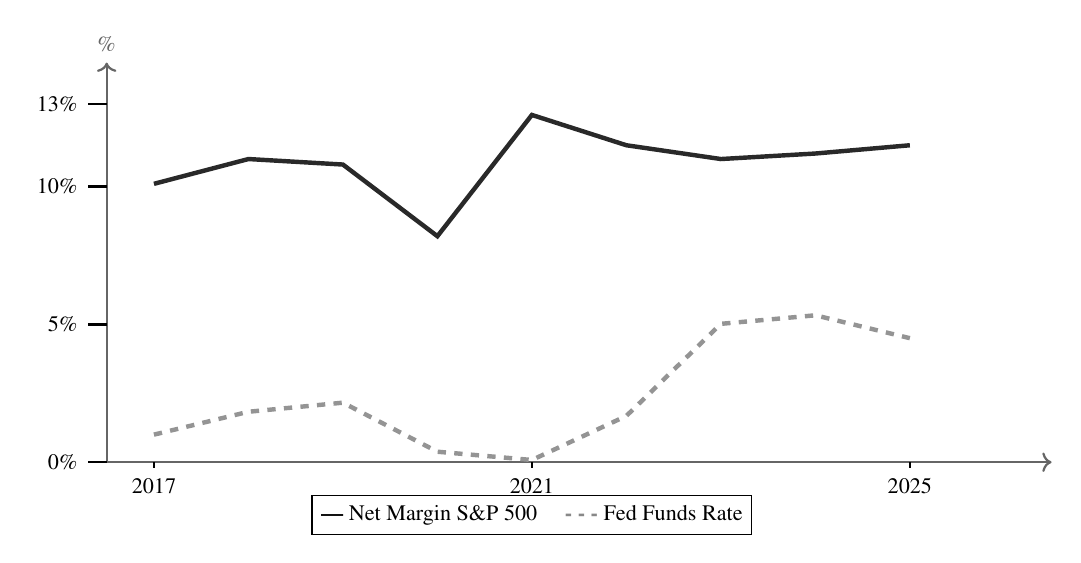
\begin{tikzpicture}[x=1.2cm, y=0.35cm]
% Draw axes
\draw[->, thick, black!60] (-0.5, 0) -- (9.5, 0);
\draw[->, thick, black!60] (-0.5, 0) -- (-0.5, 14.5) node[above, font=\footnotesize] {\%};

% Axis tick marks and labels (Tahun) - only start, middle, and end to avoid clutter
\draw[thick] (0, 0) -- (0, -0.2) node[below, font=\footnotesize] {2017};
\draw[thick] (4, 0) -- (4, -0.2) node[below, font=\footnotesize] {2021};
\draw[thick] (8, 0) -- (8, -0.2) node[below, font=\footnotesize] {2025};

% Y-axis labels - only bottom and top
\draw[thick] (-0.5, 0) -- (-0.7, 0) node[left, font=\footnotesize] {0\%};
\draw[thick] (-0.5, 5) -- (-0.7, 5) node[left, font=\footnotesize] {5\%};
\draw[thick] (-0.5, 10) -- (-0.7, 10) node[left, font=\footnotesize] {10\%};
\draw[thick] (-0.5, 13) -- (-0.7, 13) node[left, font=\footnotesize] {13\%};

% Net Margin line (AksaBlue)
\draw[AksaBlue!90, ultra thick, mark=*]
  (0, 10.1) -- (1, 11.0) -- (2, 10.8) -- (3, 8.2) -- (4, 12.6) -- (5, 11.5) -- (6, 11.0) -- (7, 11.2) -- (8, 11.5);

% Fed Funds Rate line (AksaOrange)
\draw[AksaOrange!90, ultra thick, dashed, mark=square*]
  (0, 1.00) -- (1, 1.83) -- (2, 2.16) -- (3, 0.38) -- (4, 0.08) -- (5, 1.68) -- (6, 5.02) -- (7, 5.33) -- (8, 4.50);

% Legend at the bottom, clean and uncluttered
\node[draw, fill=white, font=\footnotesize, anchor=north] at (4, -1.2) {
  \textcolor{AksaBlue}{\textbf{---}} Net Margin S\&P 500 \quad
  \textcolor{AksaOrange}{\textbf{- - -}} Fed Funds Rate
};
\end{tikzpicture}
\vspace{1.5em}
{\small Sumber: Bloomberg Terminal, Federal Reserve Board, BEA (diolah). Sumbu X menunjukkan tahun pengamatan; Sumbu Y menunjukkan persentase tingkat bunga dan margin kotor.}
\end{figure}

\begin{figure}[H]
\caption{Fenomena Gap: Persistensi Margin S\&P 500 vs Tekanan Suku Bunga (2022--2025)}
\centering
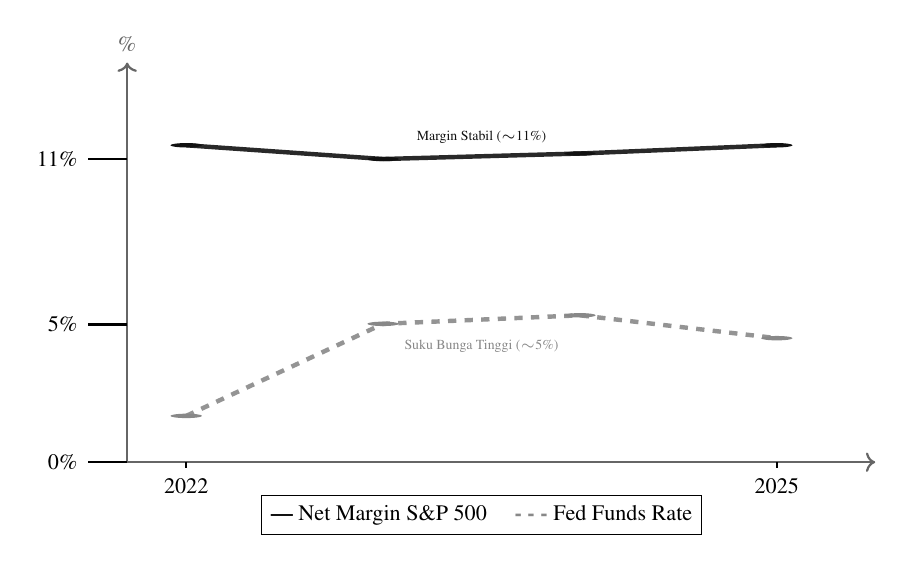
\begin{tikzpicture}[x=2.5cm, y=0.35cm]
% Draw axes
\draw[->, thick, black!60] (-0.3, 0) -- (3.5, 0);
\draw[->, thick, black!60] (-0.3, 0) -- (-0.3, 14.5) node[above, font=\footnotesize] {\%};

% Axis tick marks and labels (Tahun) - only start and end
\draw[thick] (0, 0) -- (0, -0.2) node[below, font=\footnotesize] {2022};
\draw[thick] (3, 0) -- (3, -0.2) node[below, font=\footnotesize] {2025};

% Y-axis labels - only key margins
\draw[thick] (-0.3, 0) -- (-0.5, 0) node[left, font=\footnotesize] {0\%};
\draw[thick] (-0.3, 5) -- (-0.5, 5) node[left, font=\footnotesize] {5\%};
\draw[thick] (-0.3, 11) -- (-0.5, 11) node[left, font=\footnotesize] {11\%};

% Actual Margin (Sustained)
\draw[AksaBlue!90, ultra thick]
  (0, 11.5) -- (1, 11.0) -- (2, 11.2) -- (3, 11.5);
\fill[AksaBlue] (0,11.5) circle (0.08);
\fill[AksaBlue] (1,11.0) circle (0.08);
\fill[AksaBlue] (2,11.2) circle (0.08);
\fill[AksaBlue] (3,11.5) circle (0.08);

% Fed Rate (dashed)
\draw[AksaOrange!90, ultra thick, dashed]
  (0, 1.68) -- (1, 5.02) -- (2, 5.33) -- (3, 4.50);
\fill[AksaOrange] (0,1.68) circle (0.08);
\fill[AksaOrange] (1,5.02) circle (0.08);
\fill[AksaOrange] (2,5.33) circle (0.08);
\fill[AksaOrange] (3,4.50) circle (0.08);

% Labels for gap at the end
\node[font=\tiny, AksaBlue, anchor=south] at (1.5, 11.2) {Margin Stabil ($\sim$11\%)};
\node[font=\tiny, AksaOrange, anchor=north] at (1.5, 4.8) {Suku Bunga Tinggi ($\sim$5\%)};

% Legend
\node[draw, fill=white, font=\footnotesize, anchor=north] at (1.5, -1.2) {
  \textcolor{AksaBlue}{\textbf{---}} Net Margin S\&P 500 \quad
  \textcolor{AksaOrange}{\textbf{- - -}} Fed Funds Rate
};
\end{tikzpicture}
\vspace{1.5em}
{\small Sumber: Bloomberg Terminal dan Federal Reserve Board (diolah). Margin tetap kokoh di atas 11\% meski suku bunga Federal Reserve melonjak secara agresif ke kisaran 5,33\%.}
\end{figure}

\begin{figure}[H]
\caption{Dekomposisi Persistensi Laba: Distribusi Perusahaan S\&P 500 Berdasarkan Konsistensi SROA (2019--2025)}
\centering
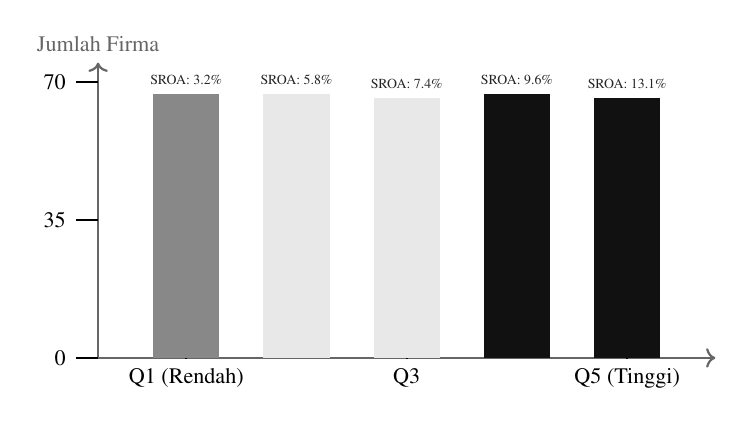
\begin{tikzpicture}[x=1.4cm, y=0.05cm]
% Draw axes
\draw[->, thick, black!60] (0.2, 0) -- (5.8, 0);
\draw[->, thick, black!60] (0.2, 0) -- (0.2, 75) node[above, font=\footnotesize] {Jumlah Firma};

% Axis tick marks and labels
\draw[thick] (1, 0) -- (1, -0.1) node[below, font=\footnotesize] {Q1 (Rendah)};
\draw[thick] (3, 0) -- (3, -0.1) node[below, font=\footnotesize] {Q3};
\draw[thick] (5, 0) -- (5, -0.1) node[below, font=\footnotesize] {Q5 (Tinggi)};

% Y-axis labels - only bottom and top
\draw[thick] (0.2, 0) -- (0.0, 0) node[left, font=\footnotesize] {0};
\draw[thick] (0.2, 35) -- (0.0, 35) node[left, font=\footnotesize] {35};
\draw[thick] (0.2, 70) -- (0.0, 70) node[left, font=\footnotesize] {70};

% Bars - simple, neat, consistent width and spacing
\foreach \x/\val/\sroa/\col in {
  1/67/3.2/AksaOrange,
  2/67/5.8/AksaSand,
  3/66/7.4/AksaSand,
  4/67/9.6/AksaBlue,
  5/66/13.1/AksaBlue}
{
  \fill[\col] (\x-0.3, 0) rectangle (\x+0.3, \val);
  % SROA value inside or on top, without overlap
  \node[above, font=\tiny, black!85] at (\x, \val) {SROA: \sroa\%};
}
\end{tikzpicture}
\vspace{1.5em}
{\small Q1 = paling inkonsisten (SROA volatil), Q5 = paling persisten. Firma kuintil teratas mencatat rata-rata SROA 13,1\% vs 3,2\% pada kuintil bawah.}
\end{figure}

\begin{table}[H]
\caption{Tren Kinerja Profitabilitas S\&P 500 dan Indikator Turbulensi Makroekonomi Amerika Serikat (2017--2025)}
\label{tab:makro-turbulensi}
\centering
\begin{tabularx}{\textwidth}{c c c c c >{\raggedright\arraybackslash}X}
\toprule
\textbf{Tahun} & \textbf{Net Margin (\%)} & \textbf{Fed Funds (\%)} & \textbf{PDB (\%)} & \textbf{Inflasi (\%)} & \textbf{Konteks Makroekonomi dan Turbulensi} \\
\midrule
2017 & 10,1 & 1,00 & 2,3 & 2,1 & Era ekspansi stabil pra-pandemi; deregulasi pajak (*Tax Cuts and Jobs Act*). \\
2018 & 11,0 & 1,83 & 2,9 & 2,4 & Pengetatan moneter moderat; eskalasi perang dagang AS-Tiongkok. \\
2019 & 10,8 & 2,16 & 2,3 & 1,8 & Perlambatan global; Federal Reserve mulai menurunkan suku bunga (*insurance cuts*). \\
2020 & 8,2 & 0,38 & -3,4 & 1,2 & *COVID-19 Shock*; resesi ekonomi; Fed menurunkan suku bunga ke batas bawah nol (ZIRP) dan QE masif. \\
2021 & 12,6 & 0,08 & 5,7 & 4,7 & *Post-Pandemic Demand Boom*; pelonggaran likuiditas; disrupsi rantai pasok global memicu *pricing power*. \\
2022 & 11,5 & 1,68 & 1,9 & 8,0 & Perang Rusia-Ukraina memicu krisis energi; inflasi melonjak; Fed memulai siklus kenaikan suku bunga agresif. \\
2023 & 11,0 & 5,02 & 2,5 & 4,1 & Lanjutan pengetatan moneter; Fed menaikkan suku bunga ke kisaran 5,25\%--5,50\%; krisis perbankan regional. \\
2024 & 11,2 & 5,33 & 2,7 & 2,9 & *Sustained margins*; disrupsi rantai pasok mereda; antusiasme teknologi *Artificial Intelligence* (AI). \\
2025 & 11,5 & 4,50 & 2,1 & 2,4 & Normalisasi inflasi; siklus pelonggaran moneter bertahap (*soft landing*). \\
\bottomrule
\end{tabularx}
\vspace{0.5em}
{\small Sumber: Bloomberg, Bureau of Economic Analysis (BEA), dan Federal Reserve Board (diolah).}
\end{table}

Tabel 1.1 membagi pengamatan makroekonomi AS menjadi empat fase krusial:
(1) Fase pertumbuhan stabil pra-pandemi (2017--2019) yang diiringi
kebijakan fiskal ekspansif; (2) Fase guncangan pandemi COVID-19 (2020)
di mana aktivitas ekonomi terhenti, menyebabkan resesi mendalam tetapi
langsung dimitigasi dengan pemotongan suku bunga acuan mendekati 0\%
(ZIRP) dan program pelonggaran kuantitatif (QE) tanpa batas oleh Federal
Reserve; (3) Fase pemulihan ekonomi pasca-pandemi (\emph{post-pandemic
demand boom}) tahun 2021--2022 yang memicu lonjakan permintaan di tengah
kemacetan rantai pasok global, menghasilkan keuntungan luar biasa
(\emph{windfall profits}) bagi korporasi besar; dan (4) Fase pengetatan
moneter paling agresif dalam sejarah modern (2022--2025) di mana Federal
Reserve mengerek suku bunga acuan hingga menyentuh kisaran
5,25\%--5,50\% demi meredam tingkat inflasi tertinggi dalam 40 tahun
terakhir.

Di tengah skenario turbulensi makroekonomi yang luar biasa berat
tersebut, terbentuk sebuah kesenjangan fenomena (\emph{phenomena gap})
yang sangat kontras dan menarik untuk ditelaah dari perspektif
ekonometrika keuangan. Teori ekonomi makro konvensional secara apriori
memprediksi bahwa kombinasi dari inflasi beban biaya (\emph{cost-push
inflation}), biaya utang yang melonjak tinggi akibat suku bunga acuan
Federal Reserve yang menyentuh level 5,50\%, serta normalisasi
permintaan pasca-pandemi seharusnya menggerus margin profitabilitas
korporasi secara drastis karena kenaikan biaya operasional yang
melampaui pertumbuhan penjualan. Namun, kenyataan empiris pada pasar
modal Amerika Serikat menunjukkan anomali yang sangat mencolok, di mana
margin laba bersih rata-rata korporasi konstituen S\&P 500 justru
terbukti tangguh dan mampu bertahan kokoh pada tingkat yang tinggi,
mencapai angka 11,2\% pada akhir tahun 2024 dan tetap stabil di atas
11,5\% pada tahun 2025. Ketahanan profitabilitas yang luar biasa di
tengah gejolak biaya modal ini melahirkan teka-teki teoretis yang
mendalam bagi akademisi dan praktisi keuangan korporat. Mengapa
emiten-emiten berskala besar di Amerika Serikat seakan memiliki imunitas
keuangan terhadap kenaikan biaya dana dan inflasi ekstrem? Apakah
ketahanan profitabilitas berkelanjutan ini ditopang oleh perlindungan
struktur oligopolistik eksternal pasar mereka (\emph{Market-Based View}
/ SCP) yang memampukan petahana membebankan inflasi biaya langsung
kepada konsumen melalui koordinasi pasar tacit (\emph{pricing power}
sektoral), ataukah ditopang oleh keunggulan kapabilitas fundamental
kualitas keuangan internal perusahaan itu sendiri (\emph{Resource-Based
View} / RBV) melalui optimalisasi struktur neraca dan efisiensi
operasional?

Kesenjangan penelitian (\emph{research gap}) dalam topik ini bersumber
dari ketidakkonsistenan temuan empiris terdahulu serta kelemahan
metodologis yang ada dalam literatur empiris keuangan korporat dan
organisasi industri. Di satu sisi, banyak studi empiris klasik maupun
modern, seperti Pervan, Pervan, dan Curak (2019) serta berbagai
pendukung teori ekonomi industri tradisional, menyokong keabsahan
paradigma SCP dengan menemukan korelasi positif dan signifikan secara
statistik antara konsentrasi industri dan kinerja laba perusahaan.
Mereka berargumen bahwa konsentrasi pasar yang tinggi mempermudah
terjadinya kolusi diam-diam dan menurunkan intensitas persaingan,
sehingga secara langsung menaikkan profitabilitas. Sebaliknya, kritik
fundamental yang diajukan oleh Harold Demsetz (1973) melalui teori
\emph{efficiency structure hypothesis} (ESH) membantah penjelasan SCP
tersebut. Demsetz mengingatkan bahwa tingkat konsentrasi industri yang
tinggi sebenarnya merupakan hasil alamiah dari efisiensi operasional
superior dan kualitas internal perusahaan individual yang sukses merebut
pangsa pasar dari pesaing yang kurang efisien, bukan semata-mata
cerminan rente monopoli atau perilaku kolutif pelaku usaha dominan.
Dengan kata lain, hubungan positif antara konsentrasi pasar dan
profitabilitas merupakan cerminan dari superioritas efisiensi internal
perusahaan (\emph{firm-level efficiency}), bukan akibat langsung dari
perlindungan kekuatan pasar eksternal (\emph{industry-level market
power}).

Ketidakkonsistenan temuan empiris ini diperkuat oleh studi dekomposisi
varians kinerja keuangan korporasi yang dipelopori oleh Anita McGahan
dan Michael Porter (1997) serta studi lanjutan oleh Goddard dkk. (2011)
yang menganalisis persistensi laba perusahaan dalam jangka panjang.
Penelitian mereka secara konsisten membuktikan bahwa efek spesifik
perusahaan (\emph{firm-specific effects}) memiliki kontribusi yang jauh
lebih dominan dan persisten dalam menjelaskan variabilitas
profitabilitas berkelanjutan dibandingkan dengan efek industri
(\emph{industry-specific effects}). Temuan monumental ini menegaskan
bahwa ``bagaimana suatu perusahaan dikelola secara internal'' dan
bagaimana parit ekonomi internal dikembangkan jauh lebih krusial dalam
mempertahankan kelangsungan laba dibandingkan ``di mana sektor industri
tempat perusahaan tersebut terdaftar atau beroperasi''. Meskipun
demikian, integrasi dan kontestasi langsung antara efek konsentrasi
industri eksternal dan kapabilitas keuangan internal dalam iklim suku
bunga tinggi paska-pandemi masih sangat jarang dievaluasi secara
simultan dalam satu model estimasi panel tunggal. Kesenjangan empiris
ini menyisakan ruang perdebatan ekonometrika yang perlu diselidiki lebih
lanjut, terutama karena dinamika pasar modern saat ini didominasi oleh
perusahaan teknologi dan jasa padat modal intelektual yang memiliki
model parit ekonomi yang berbeda secara fundamental dari perusahaan
manufaktur era industri klasik yang menjadi dasar pembentukan paradigma
SCP mula-mula.

Selain perdebatan empiris tersebut, penelitian terdahulu di bidang
manajemen keuangan dan akuntansi umumnya memiliki kelemahan metodologis
berupa penggunaan indikator rasio keuangan tunggal yang terfragmentasi
dan diuji secara terpisah.
\hl{Studi-studi klasik maupun kontemporer, seperti penelitian pelopor dari Beaver (1966) mengenai rasio tunggal untuk prediksi kebangkrutan, Rajan dan Zingales (1995) yang menguji pengaruh leverage, serta Salim dan Yadav (2012) yang menganalisis kinerja keuangan secara terfragmentasi, umumnya menguji rasio leverage secara terpisah atau hanya menggunakan rasio profitabilitas aset secara parsial}
untuk merepresentasikan kualitas internal perusahaan. Pendekatan parsial
ini gagal menangkap dimensi kualitas keuangan internal secara holistik
karena masing-masing rasio keuangan memiliki kelemahan inheren dan
rentan mengalami bias spesifikasi model. Penelitian ini mengatasi
kelemahan metodologis tersebut dengan memperkenalkan indeks komposit
kontinu \emph{Business Quality Score} (BQS) yang mengintegrasikan lima
pilar keuangan utama secara simultan: margin kotor, margin arus kas
bebas, disiplin leverage, kapasitas proteksi bunga, dan konsistensi laba
berjalan. Dengan menggabungkan kelima dimensi ini ke dalam satu skor
kontinu terstandarisasi melalui transformasi Z-score, BQS mampu
merepresentasikan kekuatan parit ekonomi (\emph{economic moat}) dan
kapabilitas internal perusahaan secara komprehensif tanpa terjebak dalam
bias spesifikasi rasio tunggal yang sering kali mendistorsi hasil
estimasi karena kegagalan menangkap interaksi komplementer antar rasio
keuangan di dalam laporan laba rugi dan neraca korporasi.

Untuk menghasilkan estimasi parameter yang tidak bias dan dapat
dipertanggungjawabkan secara ekonometrika, penelitian ini menerapkan
pendekatan estimasi model \emph{Two-way Fixed Effects} (FE) pada data
panel longitudinal. Pendekatan ini secara ketat mengontrol bias
parameter akibat variabel tak terobservasi yang konstan lintas waktu
pada level perusahaan (\emph{firm fixed effects} seperti reputasi
manajemen, budaya kerja, parit teknologi) serta menyerap dampak
guncangan makroekonomi tahunan yang bersifat umum (\emph{year fixed
effects} seperti fluktuasi inflasi, suku bunga Federal Reserve, resesi
ekonomi global) sepanjang periode pengamatan 2017--2025. Koreksi
standard error dilakukan menggunakan penyesuaian kovarians
\emph{Firm-Clustered Robust Standard Errors} berdasarkan kerangka kerja
Mitchell Petersen (2009) yang secara disiplin mengatasi gangguan
autokorelasi serial intra-firma lintas waktu dan heteroskedastisitas
residual, sehingga menghasilkan nilai standard error yang tidak bias dan
menjamin bahwa p-value dalam pengujian hipotesis bersifat sangat
defensif, konservatif, dan valid. Atas dasar pemikiran teoretis dan
metodologis yang terintegrasi secara mendalam tersebut, penelitian ini
dilaksanakan dengan judul resmi: \textbf{``Determinan Profitabilitas
Berkelanjutan Perusahaan Konstituen S\&P 500''}.

\subsection{Rumusan Masalah}\label{rumusan-masalah}

Berangkat dari latar belakang masalah yang telah dipaparkan, inti
permasalahan dalam penelitian ini adalah adanya dualisme perspektif
teoretis dan ketidakpastian empiris mengenai penentu dominan
profitabilitas berkelanjutan korporasi raksasa di era turbulensi
makroekonomi. Apakah tingkat pengembalian laba di atas normal yang
persisten lebih ditentukan oleh posisi perlindungan eksternal di dalam
struktur industri yang terkonsentrasi murni (SCP), ataukah oleh daya
tahan dan keunggulan kapabilitas keuangan internal perusahaan (RBV). Hal
ini sangat relevan untuk diteliti mengingat kurun waktu 2017--2025
diwarnai guncangan moneter dan inflasi ekstrem yang menguji batas
imunitas keuangan korporasi konstituen S\&P 500.

Berdasarkan perumusan masalah tersebut, pertanyaan penelitian dirumuskan
secara formal sebagai berikut: 1. Apakah struktur industri, yang
diproksikan dengan tingkat konsentrasi pasar (\emph{Herfindahl-Hirschman
Index} - \(HHI_{j,t}\)), berpengaruh signifikan terhadap profitabilitas
berkelanjutan (\(SROA_{i,t}\)) perusahaan konstituen S\&P 500? 2. Apakah
kualitas bisnis, yang diproksikan dengan skor komposit kualitas bisnis
(\emph{Business Quality Score} - \(BQS_{i,t}\)), berpengaruh signifikan
terhadap profitabilitas berkelanjutan (\(SROA_{i,t}\)) perusahaan
konstituen S\&P 500? 3. Di antara struktur industri eksternal
(\(HHI_{j,t}\)) dan kualitas bisnis internal (\(BQS_{i,t}\)), faktor
manakah yang memberikan kontribusi relatif lebih dominan dalam
menjelaskan variasi profitabilitas berkelanjutan (\(SROA_{i,t}\))
perusahaan konstituen S\&P 500 pada model panel yang diestimasi?

\subsection{Tujuan dan Kegunaan
Penelitian}\label{tujuan-dan-kegunaan-penelitian}

\textbf{Tujuan Penelitian.} Berdasarkan pertanyaan penelitian yang telah
dirumuskan, tujuan yang ingin dicapai dalam penelitian ini adalah: 1.
Menganalisis dan membuktikan secara empiris pengaruh struktur industri
(\(HHI_{j,t}\)) terhadap profitabilitas berkelanjutan (\(SROA_{i,t}\))
perusahaan konstituen S\&P 500. 2. Menganalisis dan membuktikan secara
empiris pengaruh kualitas bisnis (\(BQS_{i,t}\)) terhadap profitabilitas
berkelanjutan (\(SROA_{i,t}\)) perusahaan konstituen S\&P 500. 3.
Menganalisis dan membandingkan tingkat dominansi relatif antara faktor
struktur industri (\(HHI_{j,t}\)) dan kualitas bisnis (\(BQS_{i,t}\))
dalam menjelaskan variasi profitabilitas berkelanjutan (\(SROA_{i,t}\))
perusahaan konstituen S\&P 500.

\textbf{Kegunaan Penelitian.} Penyelidikan empiris ini diharapkan
memberikan manfaat dan kegunaan ilmiah yang mencakup dua aspek utama:

\begin{enumerate}
\def\labelenumi{\arabic{enumi}.}
\tightlist
\item
  \textbf{Kegunaan Teoritis (Akademis)}:

  \begin{itemize}
  \tightlist
  \item
    \textbf{Pengayaan Literatur Dualisme SCP vs RBV}: Hasil penelitian
    ini diharapkan dapat memperkaya perdebatan teoretis antara mazhab
    SCP dan RBV di era modern. Khususnya, menunjukkan bagaimana
    interaksi kedua paradigma ini bekerja di bawah tekanan guncangan
    makroekonomi yang berat dan pergeseran struktur ekonomi yang semakin
    padat modal intelektual.
  \item
    \textbf{Validasi Metodologis Penggunaan Indeks BQS}: Penelitian ini
    memberikan validasi metodologis atas penggunaan indikator komposit
    formatif \emph{Business Quality Score} (BQS) untuk memproksikan
    kualitas keuangan perusahaan, menawarkan alternatif yang lebih
    komprehensif daripada indikator keuangan tunggal konvensional yang
    rentan terhadap bias spesifikasi.
  \item
    \textbf{Pencegahan Bias Parameter}: Menunjukkan efektivitas
    penggunaan pemodelan data panel dengan estimator \emph{Two-way Fixed
    Effects} dalam mereduksi bias variabel terlewat (\emph{omitted
    variable bias}).
  \end{itemize}
\item
  \textbf{Kegunaan Praktis}:

  \begin{itemize}
  \tightlist
  \item
    \textbf{Bagi Investor dan Manajer Investasi}: Menyediakan landasan
    analitis kuantitatif dalam menyusun bobot alokasi aset portofolio
    global. Hasil studi membantu investor menentukan apakah alokasi aset
    harus menitikberatkan pada pemilihan sektor industri strategis yang
    oligopolistik atau pada pemilihan emiten dengan fundamental keuangan
    superior.
  \item
    \textbf{Bagi Manajemen Korporasi (C-Suite)}: Menjadi acuan bagi
    manajemen tingkat tinggi dalam memformulasikan kebijakan strategis
    internal. Temuan ini menegaskan pentingnya menjaga kedisiplinan
    keuangan (seperti margin laba, konversi kas, stabilitas leverage,
    kapasitas bunga, dan konsistensi kinerja) untuk membangun pertahanan
    internal yang kokoh.
  \item
    \textbf{Bagi Regulator dan Otoritas Persaingan Usaha (FTC/DOJ)}:
    Memberikan masukan ilmiah dalam mengevaluasi kebijakan antimonopoli
    dan merger korporasi secara hati-hati, guna membedakan secara
    empiris apakah profitabilitas tinggi merupakan hasil dari kolusi
    pasar yang merugikan kesejahteraan konsumen atau cerminan efisiensi
    ekonomi superior dari kualitas internal korporasi.
  \end{itemize}
\end{enumerate}

\subsection{Sistematika Penulisan}\label{sistematika-penulisan}

Penulisan skripsi ini disusun secara sistematis ke dalam lima bab utama
untuk mempermudah pemahaman alur berpikir deduktif yang terstruktur:

\textbf{BAB I: PENDAHULUAN}

Menjelaskan latar belakang masalah yang melandasi pentingnya penelitian,
rumusan masalah, pertanyaan penelitian, tujuan dan kegunaan penelitian,
serta sistematika penulisan skripsi.

\textbf{BAB II: TINJAUAN PUSTAKA}

Menyajikan telaah literatur teori terkait \emph{Persistence of Profit},
SCP, RBV, justifikasi konstruksi variabel komposit BQS, rangkuman
penelitian empiris terdahulu, kerangka pemikiran teoretik, dan perumusan
hipotesis.

\textbf{BAB III: METODE PENELITIAN}

Menguraikan desain penelitian, variabel penelitian dan definisi
operasional, populasi dan sampel, jenis dan sumber data, metode
pengumpulan data, serta tahapan analisis data panel ekonometrika.

\textbf{BAB IV: HASIL DAN ANALISIS}

Menyajikan deskripsi data objek penelitian, hasil pengujian asumsi dan
pemilihan model, estimasi parameter \emph{Two-way Fixed Effects}, serta
pembahasan teoretis dan ekonomi atas temuan empiris.

\textbf{BAB V: PENUTUP}

Menyajikan kesimpulan akhir dari temuan penelitian, implikasi teoritis
dan praktis, keterbatasan penelitian yang dihadapi, serta saran untuk
penelitian mendatang.

\begin{center}\rule{0.5\linewidth}{0.5pt}\end{center}

\section{TINJAUAN PUSTAKA}\label{tinjauan-pustaka}

\subsection{Literatur Teori}\label{literatur-teori}

Analisis ekonometrika mengenai profitabilitas berkelanjutan diletakkan
di atas fondasi teoretis ekonomi industri dan manajemen keuangan yang
mapan. Untuk menguji daya penjelas relatif antara kekuatan eksternal
industri dan keunggulan internal perusahaan, tinjauan pustaka ini
disusun secara deduktif, dimulai dari teori dasar persistensi laba,
dilanjutkan dengan bedah teoretis paradigma
\emph{Structure-Conduct-Performance} (SCP) dan \emph{Resource-Based
View} (RBV), hingga perumusan justifikasi ilmiah konstruksi variabel
komposit \emph{Business Quality Score} (BQS).

\subsubsection{Persistence of Profit}\label{persistence-of-profit}

Teori Persistensi Laba yang dikembangkan oleh Dennis Mueller (1977,
1986) merupakan antitesis terhadap \emph{Competitive Environment
Hypothesis} dalam ekonomi mikro neoklasik konvensional. Dalam model
persaingan neoklasik klasik, diasumsikan bahwa setiap tingkat keuntungan
abnormal (baik positif maupun negatif) akan mengalami pembalikan ke
nilai rata-rata (\emph{mean reversion}) dengan cepat. Jika sebuah
perusahaan memperoleh keuntungan di atas normal, tidak adanya hambatan
masuk akan mendorong masuknya pesaing baru yang meningkatkan pasokan
output, memicu persaingan harga, dan menekan tingkat profitabilitas
kembali ke titik ekuilibrium jangka panjang (laba ekonomi nol atau biaya
modal).

Mueller (1986) membantah asumsi penyederhanaan tersebut dengan
mengajukan premis bahwa friksi pasar yang riil---seperti hambatan masuk
struktural, asimetri informasi, paten, loyalitas merek, dan biaya
beralih (\emph{switching costs})---membuat proses persaingan berjalan
lambat, tidak sempurna, atau bahkan asimetris sepanjang waktu.
Akibatnya, kelompok perusahaan tertentu yang memiliki keunggulan
kompetitif superior dapat mempertahankan tingkat laba di atas rata-rata
industri secara persisten selama bertahun-tahun.
\hl{Dalam literatur ekonometrika keuangan, teori persistensi laba ini diformulasikan secara matematis melalui model autoregressive orde pertama AR(1) sebagai berikut:
}$$SROA_{i,t} = \lambda_0 + \lambda_1 SROA_{i,t-1} + \epsilon_{i,t}$$\hl{
Di mana }$SROA_{i,t}$\hl{ adalah profitabilitas berkelanjutan perusahaan }$i$\hl{ pada periode }$t$\hl{, }$SROA_{i,t-1}$\hl{ adalah profitabilitas pada periode sebelumnya, }$\lambda_0$\hl{ menunjukkan tingkat keuntungan ekuilibrium jangka panjang, }$\lambda_1$\hl{ adalah parameter kecepatan penyesuaian (*speed of adjustment*), dan }$\epsilon_{i,t}$\hl{ adalah error term. Jika }$\lambda_1 = 0$\hl{, maka profitabilitas bersifat tidak persisten dan langsung mengalami pembalikan rata-rata (*mean reversion*) secara instan ke kondisi persaingan sempurna. Sebaliknya, jika }$\lambda_1 > 0$\hl{ dan signifikan, terdapat persistensi laba di atas normal. Jika }$\lambda_1 \rightarrow 1$\hl{, kondisi pasar mengalami kelumpuhan kompetisi yang parah di mana keuntungan abnormal bertahan secara permanen.}
Hal inilah yang mendasari penggunaan metrik rata-rata bergerak
multi-tahun (\(SROA_{i,t}\)) dalam penelitian ini untuk mengekstrak
komponen laba permanen (\emph{Sustained Earnings}) perusahaan dan
meredam noise akrual transitori jangka pendek.

\subsubsection{Structure-Conduct-Performance
(SCP)}\label{structure-conduct-performance-scp}

Paradigma \emph{Structure-Conduct-Performance} (SCP) yang dipelopori
oleh Mason (1939) dan Bain (1956) merupakan kerangka kerja teoretis
utama yang memandang profitabilitas dari sudut pandang eksternal pasar.
Paradigma ini menetapkan alur kausalitas linear searah: Struktur Pasar
(\(\text{Structure}\)) \(\rightarrow\) Perilaku Perusahaan
(\(\text{Conduct}\)) \(\rightarrow\) Kinerja Ekonomi
(\(\text{Performance}\)). Struktur pasar dicirikan oleh tingkat
konsentrasi industri, hambatan masuk bagi pemain baru, dan tingkat
diferensiasi produk. Perilaku mencakup kebijakan harga, strategi iklan,
dan kolusi. Kinerja diukur dari profitabilitas dan efisiensi alokatif.

Dalam kerangka SCP, konsentrasi industri yang tinggi (diproksikan dengan
\(HHI\) tinggi) memfasilitasi terjadinya koordinasi diam-diam
(\emph{tacit collusion}) di antara perusahaan-perusahaan besar untuk
menghindari perang harga yang merugikan. Struktur oligopolistik ini
menciptakan kekuatan pasar (\emph{market power}) bagi petahana,
memampukan mereka menetapkan harga jual produk di atas biaya marjinal
(\(P > MC\)) tanpa kehilangan pangsa pasar yang signifikan. Selain itu,
skala ekonomi yang besar dan hambatan masuk yang kuat menyulitkan
pesaing baru untuk masuk dan mendisrupsi pasar. Konsekuensinya,
perusahaan dalam industri terkonsentrasi dapat menikmati keuntungan
ekonomi supernormal yang persisten.

\hl{Secara ekonometrika dan teori ekonomi mikro, operasionalisasi variabel konsentrasi industri melalui indeks Herfindahl-Hirschman (HHI) diturunkan secara formal dari Model Oligopoli Cournot dengan perusahaan-perusahaan asimetris yang memproduksi barang homogen. Berdasarkan teori Cournot, kondisi optimasi laba untuk perusahaan }$i$\hl{ dirumuskan sebagai berikut:
}$$P(Q) + s_i P'(Q) Q = MC_i$$\hl{
Di mana }$P(Q)$\hl{ adalah harga pasar, }$Q$\hl{ adalah kuantitas industri total, }$s_i = q_i / Q$\hl{ adalah pangsa pasar perusahaan }$i$\hl{, dan }$MC_i$\hl{ adalah biaya marjinal perusahaan }$i$\hl{. Dengan mendefinisikan Indeks Lerner (}$L_i$\hl{) sebagai ukuran kekuatan pasar perusahaan }$i$\hl{, persamaan tersebut ditransformasikan secara aljabar menjadi:
}$$L_i = \frac{P - MC_i}{P} = \frac{s_i}{E}$$\hl{
Di mana }$E = - \frac{P}{Q P'(Q)}$\hl{ mewakili elastisitas harga dari permintaan pasar. Keuntungan industri agregat diperoleh dengan menghitung rata-rata tertimbang Indeks Lerner seluruh perusahaan menggunakan pangsa pasar sebagai pembobot:
}$$\sum_{i=1}^N s_i L_i = \sum_{i=1}^N \frac{s_i^2}{E} = \frac{HHI}{E}$$\hl{
Di mana }$HHI = \sum_{i=1}^N s_i^2$\hl{ adalah indeks konsentrasi Herfindahl-Hirschman yang berkisar antara 0 hingga 1. Persamaan (2.2) membuktikan secara formal korelasi positif linier langsung antara HHI dan margin keuntungan industri rata-rata (indeks Lerner industri). George Stigler (1964) melalui teori kolusi oligopolinya memperkuat argumentasi ini dengan menjelaskan bahwa semakin tinggi konsentrasi pasar (semakin sedikit jumlah pemain dominan), semakin mudah bagi korporasi untuk melakukan deteksi atas penyimpangan kesepakatan tacit (kartel terselubung) dan mengontrol koordinasi harga di pasar. Dengan demikian, derivasi teoritis variabel }$HHI$\hl{ dalam penelitian ini secara eksplisit bertumpu pada transmisi ekonomi mikro Cournot dan Stigler, di mana tingkat konsentrasi eksternal membatasi persaingan harga dan menyangga persistensi profitabilitas berkelanjutan (}$SROA$\hl{) melalui ekstraksi rente oligopolistik.}

\subsubsection{Resource-Based View (RBV)}\label{resource-based-view-rbv}

Jembatan ilmiah yang menghubungkan teori manajemen strategis murni
dengan metrik akuntansi keuangan kuantitatif didirikan di atas kebutuhan
untuk mereduksi subjektivitas dalam pengukuran kapabilitas internal
perusahaan. Selama ini, paradigma Resource-Based View (RBV) yang berakar
dari pemikiran Edith Penrose (1959) serta diformalkan oleh Jay Barney
(1991) sering kali dikritik karena sifat konstruk teoretisnya yang
abstrak dan sulit diukur secara empiris. Istilah-istilah seperti
``keunikan sumber daya,'' ``kapabilitas dinamis,'' dan ``keunggulan
kompetitif berkelanjutan'' sering kali dioperasionalisasikan secara
kualitatif melalui survei atau studi kasus yang rentan terhadap bias
interpretasi dan keterbatasan sampel. Untuk mengatasi kelemahan
tersebut, penelitian ini mentranslasikan konstruk teoretis RBV dan
kriteria VRIO (Valuable, Rare, Inimitable, Organized) Barney ke dalam
parameter akuntansi keuangan kuantitatif yang objektif, kontinu, dan
dapat direplikasi secara empiris. Dengan memanfaatkan data laporan
keuangan longitudinal dari konstituen S\&P 500, konstruk abstrak
keunggulan kompetitif diterjemahkan menjadi metrik efisiensi
operasional, disiplin alokasi modal, dan imunitas keuangan terhadap
guncangan eksternal.

Wernerfelt (1984) dan Barney (1991) memformulasikan pemikiran ini
menjadi kerangka kerja RBV. RBV menolak asumsi neoklasik bahwa sumber
daya produktif bersifat homogen lintas perusahaan dan mudah dipindahkan.
Sebaliknya, RBV mengasumsikan adanya heterogenitas sumber daya
(\emph{resource heterogeneity}) dan imobilitas sumber daya
(\emph{resource immobility}). Menurut Barney (1991), agar sumber daya
dapat menghasilkan keunggulan kompetitif berkelanjutan (\emph{sustained
competitive advantage}) yang pada akhirnya tercermin dalam
profitabilitas persisten, sumber daya tersebut harus memenuhi kriteria
VRIO: 1. \textbf{Valuable}: Mampu mengeksploitasi peluang eksternal atau
menetralkan ancaman pasar. 2. \textbf{Rare}: Unik dan tidak dimiliki
secara luas oleh para pesaing saat ini. 3. \textbf{Inimitable}: Sangat
sulit atau mahal untuk ditiru oleh kompetitor karena kompleksitas sosial
atau faktor historis unik. 4. \textbf{Organized}: Perusahaan memiliki
struktur organisasi dan sistem kontrol yang siap mengeksploitasi sumber
daya tersebut.

Dalam literatur keuangan empiris, kerangka konseptual imunitas internal
ini dioperasionalisasikan melalui konsep investasi berbasis kualitas.
Cetak biru (\emph{blueprint}) dari pemikiran ini dirumuskan oleh Asness,
Frazzini, dan Pedersen (2019) dalam konsep \emph{Quality Minus Junk}
(QMJ). Mereka membuktikan bahwa perusahaan dengan karakteristik
fundamental internal berkualitas tinggi---yang dicirikan oleh
profitabilitas tinggi, pertumbuhan stabil, leverage rendah, dan arus kas
riil---secara konsisten menghasilkan kinerja keuntungan yang unggul dan
tahan terhadap guncangan makro ekonomi.

\hl{Operasionalisasi konstruk RBV ke dalam metrik kuantitatif BQS didasarkan pada argumen bahwa keunggulan kompetitif yang tidak teramati (*unobserved competitive advantage*) secara logis harus menghasilkan jejak keuangan yang teramati (*observed financial footprint*) pada laporan keuangan perusahaan. Kriteria VRIO dari Barney (1991) dapat dipetakan secara matematis dan logis sebagai berikut: Pertama, **Value** tercermin dari kemampuan menghasilkan arus kas bebas riil yang superior (}$FCF\_MARGIN$\hl{), yang menunjukkan bahwa aset perusahaan mampu menciptakan nilai ekonomis nyata di atas biaya peluangnya. Kedua, **Rarity** dan **Inimitability** tercermin dari bertahannya margin laba kotor yang tebal (}$MARG$\hl{) lintas waktu dan konsistensi laba operasional (}$CONS$\hl{). Margin kotor yang tinggi mencerminkan keunikan penawaran produk atau kepemilikan aset tak berwujud seperti paten, merek, atau reputasi yang tidak dapat ditiru dengan mudah oleh kompetitor (causal ambiguity dan path dependency). Ketiga, **Organization** dicerminkan oleh kapabilitas manajerial dalam mengelola struktur neraca dan likuiditas (}$LEV$\hl{ dan }$INTEREST\_COVERAGE$\hl{). Struktur modal yang disiplin dan kapasitas proteksi bunga yang memadai menjamin bahwa perusahaan memiliki organisasi keuangan yang teratur dan siap mengeksploitasi peluang pasar sekaligus bertahan dari guncangan solvabilitas. Pemetaan terstruktur ini menjembatani jurang metodologis antara teori manajemen strategis kualitatif dan analisis empiris kuantitatif ekonometrika keuangan.}

\subsubsection{Konstruksi BQS dan Variabel
Kontrol}\label{konstruksi-bqs-dan-variabel-kontrol}

Konstruksi \emph{Business Quality Score} (BQS) sebagai indeks komposit
formatif didasarkan pada landasan ilmiah teoretis yang kuat untuk
masing-masing dari lima pilar keuangan penyusunnya.
\hl{Secara matematis, BQS dirumuskan sebagai rata-rata aritmetika dari Z-score masing-masing komponen yang distandardisasi secara cross-sectional setiap tahun:
}$$BQS_{i,t} = \frac{1}{5} \sum_{c=1}^5 Z(C_{c,i,t})$$\hl{
Di mana }$C_{c,i,t}$\hl{ mewakili nilai komponen keuangan ke-}$c$\hl{ untuk perusahaan }$i$\hl{ pada tahun }$t$\hl{. Transformasi Z-score dirumuskan sebagai:
}$$Z(C_{c,i,t}) = \frac{C_{c,i,t} - \mu_{c,t}}{\sigma_{c,t}}$$\hl{
Di mana }$\mu_{c,t}$\hl{ adalah rata-rata industri dari komponen }$c$\hl{ pada tahun }$t$\hl{, dan }$\sigma_{c,t}$\hl{ adalah standar deviasinya. Kelima komponen keuangan (}$C_{c,i,t}$\hl{) diturunkan secara teoritis melalui rumus akuntansi keuangan berikut:}

\begin{enumerate}
\def\labelenumi{\arabic{enumi}.}
\tightlist
\item
  \textbf{Gross Profitability Margin (\(MARG\))}:
  \hl{Pilar ini diturunkan dari Teori Persaingan Monopolistik (Chamberlin, 1933) dan Strategi Keunggulan Bersaing Porter (Porter, 1980). Secara operasional, MARG dihitung sebagai rasio laba kotor terhadap total aset:
  }$$MARG_{i,t} = \frac{\text{Laba Kotor}_{i,t}}{\text{Total Aset}_{i,t}}$$\hl{
  Dalam teori ekonomi mikro neoklasik, pasar persaingan sempurna akan memaksa harga sama dengan biaya marjinal (}$P=MC$\hl{), yang meniadakan margin abnormal. Namun, melalui diferensiasi produk yang didukung oleh aset tidak berwujud seperti paten, reputasi merek, atau teknologi eksklusif—yang dalam kerangka RBV Barney (1991) dikategorikan sebagai sumber daya yang unik (*Rare*) dan sulit ditiru (*Inimitable*)—perusahaan dapat menikmati kekuatan penetapan harga (*pricing power*) yang tebal. Hal ini memampukan mereka menetapkan harga jual jauh di atas biaya langsung barang terjual (COGS). Menurun pada Novy-Marx (2013), margin kotor merupakan proksi paling murni untuk mengukur keunggulan biaya sejati (*true cost advantage*) dan keunggulan diferensiasi operasional karena tidak terdistorsi oleh rekayasa akuntansi akrual di level laba bersih (seperti amortisasi, depresiasi, dan rekayasa pajak), sehingga merepresentasikan parit ekonomi (*economic moat*) perusahaan yang tangguh.}
\item
  \textbf{Free Cash Flow Margin (\(FCF\_MARGIN\))}:
  \hl{Diturunkan dari Teori Arus Kas Bebas (Jensen, 1986) serta Pecking Order Theory (Myers \& Majluf, 1984). FCF margin dihitung sebagai arus kas operasi bersih dikurangi pengeluaran modal (*CapEx*), dibagi dengan total penjualan:
  }$$FCF\_MARGIN_{i,t} = \frac{\text{Arus Kas Operasi}_{i,t} - \text{Capital Expenditures}_{i,t}}{\text{Total Penjualan}_{i,t}}$$\hl{
  Teori Jensen (1986) mendalilkan bahwa arus kas bebas adalah kas sisa operasional setelah membiayai seluruh proyek investasi ber-NPV positif. Dalam perspektif teori keagenan (*agency theory*), FCF margin yang tinggi merepresentasikan efisiensi alokasi modal dan otonomi manajerial perusahaan untuk mendanai ekspansi secara internal tanpa tergantung pada pasar modal eksternal yang mahal dan asimetris. Selain itu, pilar ini mewakili aspek *Value* (nilai ekonomi riil) dari kriteria VRIO. Mengacu pada kritik akrual legendaris dari Richard Sloan (1996), profitabilitas akuntansi yang tinggi sering kali bersifat transitori dan rentan mengalami pembalikan cepat (*mean reversion*) jika tidak ditopang oleh konversi kas masuk operasional yang nyata. Penggunaan margin arus kas bebas memastikan bahwa indeks BQS mengukur kualitas bisnis yang didukung oleh likuiditas kas operasional riil yang bersumber dari transaksi riil dengan pelanggan, bukan sekadar angka akrual di atas kertas.}
\item
  \textbf{Leverage Discipline (\(LEV\))}:
  \hl{Diturunkan dari Teori Struktur Modal Trade-off (Kraus \& Litzenberger, 1973) dan Teori Kelonggaran Keuangan (*Financial Slack Theory*) (Myers, 1984). Pilar LEV dioperasionalkan sebagai kebalikan dari leverage keuangan (rasio utang terhadap total aset) guna menjaga arah linearitas kualitas:
  }$$LEV_{i,t} = 1 - \frac{\text{Total Utang}_{i,t}}{\text{Total Aset}_{i,t}}$$\hl{
  Teori Trade-off menjelaskan bahwa keputusan struktur modal didasarkan pada penyeimbangan dinamis antara manfaat perlindungan pajak (*tax shield*) dan biaya kebangkrutan atau kesulitan keuangan (*financial distress costs*). Ketika Federal Reserve menaikkan suku bunga acuan secara ekstrem selama periode 2022--2025, biaya modal marginal utang meningkat drastis, sehingga perusahaan dengan leverage tinggi menghadapi guncangan solvabilitas. Berdasarkan Pecking Order Theory dan RBV, kelonggaran keuangan (*financial slack*) berupa utang rendah (nilai LEV disiplin tinggi) adalah aset strategis yang memampukan perusahaan mempertahankan fleksibilitas operasional, menghindari kebangkrutan teknis, dan mengambil peluang investasi strategis di kala pesaing yang memiliki utang tinggi terhambat oleh batasan likuiditas.}
\item
  \textbf{Interest Coverage Capacity (\(INTEREST\_COVERAGE\))}:
  \hl{Diturunkan secara formal dari Hipotesis Instabilitas Keuangan (*Financial Instability Hypothesis*) Hyman Minsky (1986). Metrik ini dihitung sebagai rasio laba sebelum bunga dan pajak (EBIT) terhadap beban bunga:
  }$$INTEREST\_COVERAGE_{i,t} = \frac{\text{EBIT}_{i,t}}{\text{Beban Bunga}_{i,t}}$$\hl{
  Minsky mengklasifikasikan postur keuangan korporasi ke dalam tiga rezim: *Hedge*, *Speculative*, dan *Ponzi*. Perusahaan dengan kapasitas proteksi bunga yang tinggi (}$INTEREST\_COVERAGE$\hl{ tinggi) dikategorikan berada dalam rezim *Hedge Finance*, di mana arus kas masuk operasional secara konsisten cukup untuk memenuhi kewajiban kontraktual berupa bunga dan pokok utang. Selama periode pengetatan moneter ketat, perusahaan di rezim spekulatif atau Ponzi akan mengalami gagal bayar akibat risiko pembiayaan kembali (*refinancing risk*). Oleh karena itu, metrik ini bertindak sebagai ukuran ketahanan batas aman solvabilitas jangka pendek (*safety-first principle*) yang secara teoritis melindungi kelangsungan kapabilitas organisasi dari kepailitan teknis akibat guncangan biaya bunga.}
\item
  \textbf{Earnings Consistency (\(CONS\))}:
  \hl{Diturunkan dari Teori Pensinyalan (*Signaling Theory*) (Spence, 1973; Bhattacharya, 1979) serta konsep Ketergantungan Jalur (*Path Dependency*) dan Keambiguan Kausal (*Causal Ambiguity*) (Reed \& DeFillippi, 1990) dalam RBV. Secara empiris, CONS dihitung dari kebalikan dari koefisien variasi (CV) margin kotor (}$MARG$\hl{) selama tiga tahun terakhir (}$t, t-1, t-2$\hl{):
  }$$CONS_{i,t} = \frac{1}{\text{CV}(MARG_{i,t..t-2})} = \frac{\mu_{MARG_{i,t..t-2}}}{\sigma_{MARG_{i,t..t-2}}}$$\hl{
  Volatilitas laba yang tinggi menunjukkan ketidakpastian operasional dan ketidakstabilan posisi pasar. Sebaliknya, konsistensi laba historis (}$CONS$\hl{ tinggi) bertindak sebagai sinyal kredibel kepada pasar mengenai bertahannya parit kompetitif (*economic moat*) korporasi. Mengacu pada Dichev dan Tang (2009), kestabilan margin kotor yang konsisten mencerminkan kelembaman pelanggan (*customer inertia*) dan adanya biaya beralih (*switching costs*) yang mengikat loyalitas konsumen lintas periode. Stabilitas operasional ini meminimalkan asimetri informasi dan biaya agensi, yang memampukan manajemen melakukan perencanaan investasi jangka panjang secara optimal tanpa terganggu oleh fluktuasi siklus bisnis makro.}
\end{enumerate}

\hl{Untuk variabel kontrol, ukuran perusahaan (}$SIZE$\hl{) diturunkan dari Teori Pertumbuhan Perusahaan Edith Penrose (Penrose, 1959) untuk mengontrol skala ekonomis (*economies of scale*), hambatan manajerial (*penrose effect*), dan kekuatan tawar-menawar (*bargaining power*), yang dirumuskan secara logaritma natural dari total aset: }$SIZE_{i,t} = \ln(\text{Total Aset}_{i,t})$\hl{. Variabel pertumbuhan penjualan (}$GROWTH$\hl{) dimasukkan untuk mengontrol siklus hidup produk (*product life cycle*) dan dinamika permintaan pasar emiten, dirumuskan sebagai persentase perubahan penjualan dari tahun sebelumnya: }$GROWTH_{i,t} = (\text{Penjualan}_{i,t} - \text{Penjualan}_{i,t-1}) / \text{Penjualan}_{i,t-1}$\hl{. Justifikasi teoritis penggunaan pembobotan sama rata (*equal-weighting*) pada indeks komposit BQS ditujukan untuk meniadakan bias *data-mining* (*data-mining penalty*) dan bias penyesuaian berlebihan (*overfitting bias*), menjamin kekuatan prediktif linier lintas sektoral, serta menjaga kesederhanaan dan replikabilitas akademis model regresi panel.}

\subsection{Literatur Empiris}\label{literatur-empiris}

Berikut adalah ringkasan penelitian empiris terdahulu yang mengkaji
determinan profitabilitas perusahaan dari perspektif struktur industri
dan karakteristik internal.

\begin{longtable}{>{\raggedright\arraybackslash}p{\dimexpr 0.28\textwidth - 2\tabcolsep} >{\raggedright\arraybackslash}p{\dimexpr 0.72\textwidth - 2\tabcolsep}}
\caption{Ringkasan Penelitian Empiris Terdahulu}\label{tab:ringkasan-penelitian-terdahulu}\\
\toprule
\textbf{Pengarang, Tahun \& Judul Karya} & \textbf{Detail Penelitian Terdahulu} \\
\midrule
\endfirsthead
\toprule
\textbf{Pengarang, Tahun \& Judul Karya} & \textbf{Detail Penelitian Terdahulu} \\
\midrule
\endhead
Pervan, Pervan, \& Ćurak (2019) \newline \textit{``Determinants of firm profitability in the Croatian manufacturing industry: Evidence from dynamic panel analysis''} &
\textbf{Metode \& Variabel:} \textit{Dynamic Panel Data} (System GMM). Y: ROA; X: HHI, ukuran perusahaan (\textit{size}), umur (\textit{age}), dan biaya tenaga kerja. \newline
\textbf{Temuan:} Menunjukkan hubungan positif dan signifikan secara statistik antara HHI dengan tingkat profitabilitas perusahaan. Hasil ini membuktikan keabsahan Paradigma \textit{Structure-Conduct-Performance} (SCP), di mana struktur pasar yang terkonsentrasi tinggi terbukti mampu memberikan ``payung pelindung'' bagi perusahaan petahana untuk menikmati profitabilitas supernormal akibat berkurangnya persaingan harga. \newline
\textbf{Relevansi:} Menjustifikasi penggunaan variabel HHI sebagai representasi kekuatan struktur industri eksternal yang valid dalam model regresi. \\
\midrule
Zeitun \& Tian (2014) \newline \textit{``Capital structure and corporate performance: Evidence from Jordan''} &
\textbf{Metode \& Variabel:} Regresi Data Panel (\textit{Fixed Effect} \& \textit{Random Effect}). Y: ROA, ROE, Tobin's Q; X: Leverage (rasio utang), ukuran (\textit{size}), pertumbuhan (\textit{growth}). \newline
\textbf{Temuan:} Menunjukkan hubungan negatif yang signifikan dan konsisten antara leverage dengan profitabilitas perusahaan. Perusahaan dengan tingkat utang rendah memiliki fleksibilitas keuangan lebih tinggi dan terhindar dari risiko \textit{financial distress}, sehingga mendukung premis \textit{Resource-Based View} (RBV) and \textit{Pecking Order Theory}. \newline
\textbf{Relevansi:} Memberikan validasi empiris yang krusial untuk memasukkan komponen Disiplin Utang (\textit{Leverage Discipline} atau LEV) sebagai salah satu pilar penentu dalam indeks komposit \textit{Business Quality Score} (BQS). \\
\midrule
Asness, Frazzini, \& Pedersen (2019) \newline \textit{``Quality minus junk''} &
\textbf{Metode \& Variabel:} \textit{Portfolio sorting} \& regresi lintas-sektoral Fama-MacBeth. Y: \textit{Stock Returns} \& Profitabilitas; X: \textit{Quality Score} (Profitabilitas, Pertumbuhan, Keamanan/\textit{safety}, dan \textit{payout}). \newline
\textbf{Temuan:} Membuktikan secara empiris bahwa saham-saham dengan karakteristik kualitas yang tinggi secara konsisten menghasilkan pengembalian (\textit{risk-adjusted returns}) yang superior dan persisten di seluruh dunia, secara signifikan mengalahkan saham-saham berkualitas rendah (\textit{junk}). \newline
\textbf{Relevansi:} Menjadi cetak biru (\textit{blueprint}) utama dalam perancangan variabel independen internal berupa \textit{Business Quality Score} (BQS), yang mentransformasikan faktor investasi kuantitatif menjadi indeks keuangan untuk mengukur kapabilitas internal perusahaan. \\
\midrule
Novy-Marx (2013) \newline \textit{``The other side of value: The gross profitability premium''} &
\textbf{Metode \& Variabel:} Regresi \textit{cross-sectional} Fama-MacBeth. Y: \textit{Stock Returns}; X: \textit{Gross Profitability} vs \textit{Net Income}. \newline
\textbf{Temuan:} Menemukan bahwa \textit{Gross Profitability} (laba kotor dibagi dengan total aset) memiliki daya penjelas (\textit{predictive power}) yang jauh lebih kuat dan stabil dalam mencerminkan keunggulan kompetitif sejati perusahaan dibandingkan dengan laba bersih (\textit{net income}) yang sering kali terdistorsi oleh kebijakan akuntansi non-operasional, beban pajak, depresiasi, dan amortisasi yang bersifat subyektif. \newline
\textbf{Relevansi:} Memberikan justifikasi metodologis bagi penelitian ini untuk menempatkan \textit{Gross Profit Margin} (MARG) sebagai indikator pertama dan utama dalam mengukur dimensi kekuatan penetapan harga (\textit{pricing power}) pada BQS. \\
\midrule
Hirsch, Schiefer, Gschwandtner, \& Hartmann (2021) \newline \textit{``Profitability and profit persistence in EU food retailing''} &
\textbf{Metode \& Variabel:} Dynamic Panel Data (System GMM). Y: ROA (mengukur koefisien kecepatan penyesuaian $\lambda$); X: ROA historis, pangsa pasar (\textit{market share}), ukuran (\textit{size}). \newline
\textbf{Temuan:} Menunjukkan tingkat persistensi laba yang sangat tinggi pada perusahaan ritel pangan skala besar. Lebih lanjut, pangsa pasar individu dan ukuran perusahaan berpengaruh positif signifikan dalam menahan laju penurunan laba (\textit{mean reversion}), membuktikan bahwa kekuatan pasar struktural dan efisiensi operasional bekerja secara simultan dalam menjaga kinerja. \newline
\textbf{Relevansi:} Memperkuat argumentasi teoretis penggunaan metrik profitabilitas multi-tahun yang dinamis untuk menangkap fenomena \textit{profit persistence} pada variabel dependen \textit{Sustained ROA}. \\
\midrule
Stephan, Talavera, \& Tsapin (2008) \newline \textit{``Persistence and Determinants of Firm Profit in Emerging Markets''} &
\textbf{Metode \& Variabel:} Model Autoregressive orde pertama AR(1) data panel. Y: ROA; X: ROA historis, ukuran, pertumbuhan, ekspor. \newline
\textbf{Temuan:} Menunjukkan bahwa profitabilitas masa lalu memiliki pengaruh signifikan terhadap profitabilitas masa depan (persistensi laba). Namun, koefisien persistensi di \textit{emerging markets} terbukti jauh lebih rendah dan tidak stabil dibanding negara maju akibat volatilitas makroekonomi, lemahnya perlindungan aset tak berwujud, dan tingginya friksi pasar. \newline
\textbf{Relevansi:} Menjustifikasi pemilihan konstituen S\&P 500 (Amerika Serikat) sebagai objek penelitian, karena pasar yang maju secara teoretis merupakan laboratorium terbaik untuk menguji pengaruh parit ekonomi internal (BQS) dan konsentrasi (HHI). \\
\midrule
Sloan (1996) \newline \textit{``Do Stock Prices Fully Reflect Information in Accruals and Cash Flows about Future Earnings?''} &
\textbf{Metode \& Variabel:} Regresi OLS \& analisis portofolio \textit{mispricing}. Y: Profitabilitas masa depan; X: Komponen akrual (\textit{accruals}) vs komponen arus kas (\textit{cash flows}). \newline
\textbf{Temuan:} Membuktikan secara empiris bahwa laba yang didominasi oleh arus kas operasional riil memiliki tingkat persistensi jauh lebih tinggi dan kualitas prediksi lebih baik dibanding laba akrual yang rentan mengalami pembalikan (\textit{mean reverting}) akibat manipulasi manajemen laba. \newline
\textbf{Relevansi:} Melandasi keputusan penelitian ini untuk memasukkan komponen \textit{Free Cash Flow Margin}—yang menghitung arus kas operasi dikurangi belanja modal (\textit{capex}) relatif terhadap penjualan—sebagai proksi esensial dalam BQS guna memastikan dimensi kualitas bisnis yang diukur berbasis pada kekuatan kas riil, bukan sekadar angka akuntansi akrual di atas kertas. \\
\midrule
Goddard, Liu, Molyneux, \& Wilson (2011) \newline \textit{``The persistence of profit''} &
\textbf{Metode \& Variabel:} Dynamic Panel Data (System GMM). Y: Profitabilitas; X: Pangsa pasar (\textit{firm-level}) vs indeks konsentrasi industri HHI (\textit{industry-level}). \newline
\textbf{Temuan:} Menyimpulkan bahwa pangsa pasar individu (yang mencerminkan efisiensi internal, keunggulan biaya, dan keunggulan kapabilitas sesuai hipotesis Demsetz) memiliki pengaruh yang jauh lebih dominan dan kokoh dalam menjelaskan variasi profitabilitas dibandingkan dengan faktor konsentrasi industri makro (HHI). \newline
\textbf{Relevansi:} Secara langsung melandasi perumusan masalah ketiga dan hipotesis ketiga (H3), yaitu menguji apakah faktor internal (BQS) lebih dominan daripada faktor eksternal (HHI) dalam ekosistem S\&P 500. \\
\midrule
Dichev \& Tang (2009) \newline \textit{``Earnings volatility and earnings predictability''} &
\textbf{Metode \& Variabel:} Analisis regresi keuangan jangka panjang. Y: Prediktabilitas laba masa depan; X: Volatilitas laba historis. \newline
\textbf{Temuan:} Menunjukkan adanya korelasi negatif yang sangat kuat antara volatilitas laba dengan prediktabilitas laba masa depan. Volatilitas margin yang tinggi menunjukkan ketidakpastian operasional yang besar, sedangkan kestabilan laba yang konsisten mencerminkan adanya parit kompetitif (\textit{economic moat}) yang mapan. \newline
\textbf{Relevansi:} Memberikan dasar empiris yang kuat bagi penelitian ini untuk mengonstruksi komponen konsistensi dalam BQS, yaitu \textit{Earnings Consistency} (CONS), yang diukur melalui kebalikan dari koefisien variasi margin laba kotor selama jendela waktu tiga tahun. \\
\midrule
McGahan \& Porter (1997) \newline \textit{``How Much Does Industry Matter, Really?''} &
\textbf{Metode \& Variabel:} Metode statistik \textit{Variance Decomposition}. Y: Profitabilitas (ROA); X: Efek perusahaan, efek industri, efek tahun. \newline
\textbf{Temuan:} Menemukan bahwa efek industri (\textit{industry effects}) menyumbang sekitar 19\% terhadap variasi kinerja perusahaan, sementara efek spesifik perusahaan (\textit{firm-specific effects}) menjelaskan porsi varians yang jauh lebih besar, yaitu mencapai sekitar 32\%. Temuan monumental ini membuktikan bahwa ``bagaimana sebuah perusahaan bersaing'' (sumber daya dan kualitas internal) jauh lebih menentukan kesuksesan finansial berkelanjutan dibandingkan dengan ``di mana perusahaan itu bersaing'' (pemilihan sektor industri). \newline
\textbf{Relevansi:} Menjadi landasan sintesis utama untuk mengantisipasi kontestasi dominasi relatif antara paradigma SCP (HHI) dan RBV (BQS), serta menjustifikasi dominasi relatif faktor internal atas faktor eksternal. \\
\bottomrule
\end{longtable}

\subsection{Hubungan Antar Variabel}\label{hubungan-antar-variabel}

Mekanisme transmisi dan interaksi teoretis antara struktur industri
eksternal (SCP), kualitas fundamental internal (RBV), dan profitabilitas
berkelanjutan dijabarkan sebagai berikut:

\subsubsection{Pengaruh Struktur Industri (HHI) terhadap Profitabilitas
Berkelanjutan}\label{pengaruh-struktur-industri-hhi-terhadap-profitabilitas-berkelanjutan}

\hl{Berdasarkan paradigma Structure-Conduct-Performance (SCP) yang dikemukakan oleh Mason (1939) dan Bain (1956), posisi pasar eksternal merupakan penentu utama kinerja keuntungan korporasi. Dalam pasar dengan konsentrasi tinggi (nilai HHI besar), persaingan cenderung bersifat non-kooperatif atau terkontrol karena sedikitnya jumlah pesaing utama. Kondisi ini menurunkan insentif persaingan harga yang destruktif dan memfasilitasi koordinasi diam-diam (tacit collusion) sebagaimana dijelaskan oleh Stigler (1964). Perusahaan dengan kekuatan pasar yang dilindungi oleh hambatan masuk struktural yang tinggi dapat mengekstrak laba monopoli atau oligopoli dengan menetapkan harga jual di atas biaya marjinal (}$P > MC$\hl{). Hal ini menahan laju penyusutan laba akibat persaingan pasar bebas, menyangga tingkat profitabilitas di atas rata-rata secara berkelanjutan (}$SROA$\hl{).}

\subsubsection{Pengaruh Kualitas Bisnis (BQS) terhadap Profitabilitas
Berkelanjutan}\label{pengaruh-kualitas-bisnis-bqs-terhadap-profitabilitas-berkelanjutan}

\hl{Dari kacamata Resource-Based View (RBV) yang dikembangkan oleh Wernerfelt (1984) dan Barney (1991), profitabilitas superior bersumber dari konfigurasi sumber daya dan kapabilitas internal unik yang memenuhi kriteria VRIO. Konstruk BQS mengukur kualitas fundamental internal ini melalui lima saluran keuangan terintegrasi. Margin kotor tebal (}$MARG$\hl{) mencerminkan pricing power hasil dari diferensiasi produk (Porter, 1980). Arus kas bebas (}$FCF\_MARGIN$\hl{) menjamin kelangsungan nilai ekonomi riil di luar angka akrual (Sloan, 1996). Disiplin leverage (}$LEV$\hl{) membatasi risiko kegagalan finansial (Kraus \& Litzenberger, 1973), sementara interest coverage (}$INTEREST\_COVERAGE$\hl{) menempatkan perusahaan dalam postur aman Hedge Finance (Minsky, 1986). Konsistensi laba (}$CONS$\hl{) bertindak sebagai sinyal parit ekonomi yang stabil terhadap fluktuasi (Dichev \& Tang, 2009). Sinergi kelima komponen ini menciptakan kekebalan terhadap guncangan biaya modal dan mempertahankan tingkat profitabilitas tinggi (}$SROA$\hl{) dalam jangka panjang.}

\subsubsection{Kontestasi Dominasi Relatif BQS (RBV) dan HHI
(SCP)}\label{kontestasi-dominasi-relatif-bqs-rbv-dan-hhi-scp}

\hl{Meskipun SCP memprediksi bahwa konsentrasi industri adalah penentu dominan, teori manajemen strategis modern (RBV) mengajukan hipotesis bahwa imunitas kapabilitas internal jauh lebih menentukan profitabilitas jangka panjang. Penelitian dekomposisi varians profitabilitas oleh McGahan dan Porter (1997) serta Rumelt (1991) membuktikan secara empiris bahwa efek spesifik perusahaan (firm-specific effects) menjelaskan bagian varians keuntungan yang jauh lebih besar dibandingkan efek industri (industry effects). Di pasar modern yang bercirikan disrupsi teknologi, hambatan masuk struktural industri (seperti regulasi atau kebutuhan modal tinggi) cenderung mudah roboh. Perusahaan yang hanya mengandalkan perlindungan industri terkonsentrasi tanpa kapabilitas internal yang unggul akan mengalami penurunan laba yang cepat ketika terdisrupsi. Sebaliknya, perusahaan dengan fundamental internal berkualitas tinggi (BQS superior) terbukti memiliki fleksibilitas strategis untuk mempertahankan keunggulan bersaingnya di industri apa pun. Oleh karena itu, pengaruh BQS terhadap SROA diproyeksikan lebih dominan, stabil, dan konsisten secara statistik dibandingkan pengaruh HHI.}

\subsubsection{Peran Pengendali SIZE dan
GROWTH}\label{peran-pengendali-size-dan-growth}

\hl{Ukuran perusahaan (}$SIZE$\hl{) dan pertumbuhan penjualan (}$GROWTH$\hl{) memiliki peran teoritis yang signifikan dalam memitigasi bias spesifikasi model. Menurut Teori Pertumbuhan Perusahaan Edith Penrose (1959), ukuran perusahaan mencerminkan akumulasi aset fisik dan manajerial yang memampukan eksploitasi skala ekonomi (*economies of scale*), menurunkan biaya transaksi rata-rata, dan memperkuat bargaining power di pasar input. Pertumbuhan penjualan (}$GROWTH$\hl{) mengontrol posisi perusahaan dalam siklus hidup produknya (*product life cycle*) dan dinamika permintaan konsumen. Peningkatan penjualan yang stabil mengindikasikan perluasan pangsa pasar dan pengakuan merek oleh pelanggan, yang berkontribusi langsung pada pertahanan profitabilitas. Pengendalian kedua variabel ini menjamin bahwa koefisien estimasi BQS dan HHI murni mencerminkan pengaruh kapabilitas internal dan struktur industri tanpa tercampur oleh efek skala dan pertumbuhan dinamis emiten.}

\subsection{Kerangka Pemikiran
Teoretik}\label{kerangka-pemikiran-teoretik}

Berdasarkan literatur teori dan literatur empiris di atas,
profitabilitas berkelanjutan (\(SROA_{i,t}\)) perusahaan diproyeksikan
dibentuk melalui dua jalur utama: Jalur Eksternal Kekuatan Pasar
berbasis paradigma SCP (diwakili oleh variabel \(HHI_{j,t}\)) dan Jalur
Internal Imunitas Keuangan berbasis paradigma RBV (diwakili oleh
variabel \(BQS_{i,t}\)). Variabel kontrol ukuran perusahaan (SIZE) dan
pertumbuhan penjualan (GROWTH) digunakan untuk mengendalikan perbedaan
skala ekonomi dan dinamika ekspansi pasar emiten agar tidak mendistorsi
koefisien estimasi parameter utama. Alur konseptual ini disajikan secara
skematis pada diagram berikut.

\begin{figure}[H]
\centering
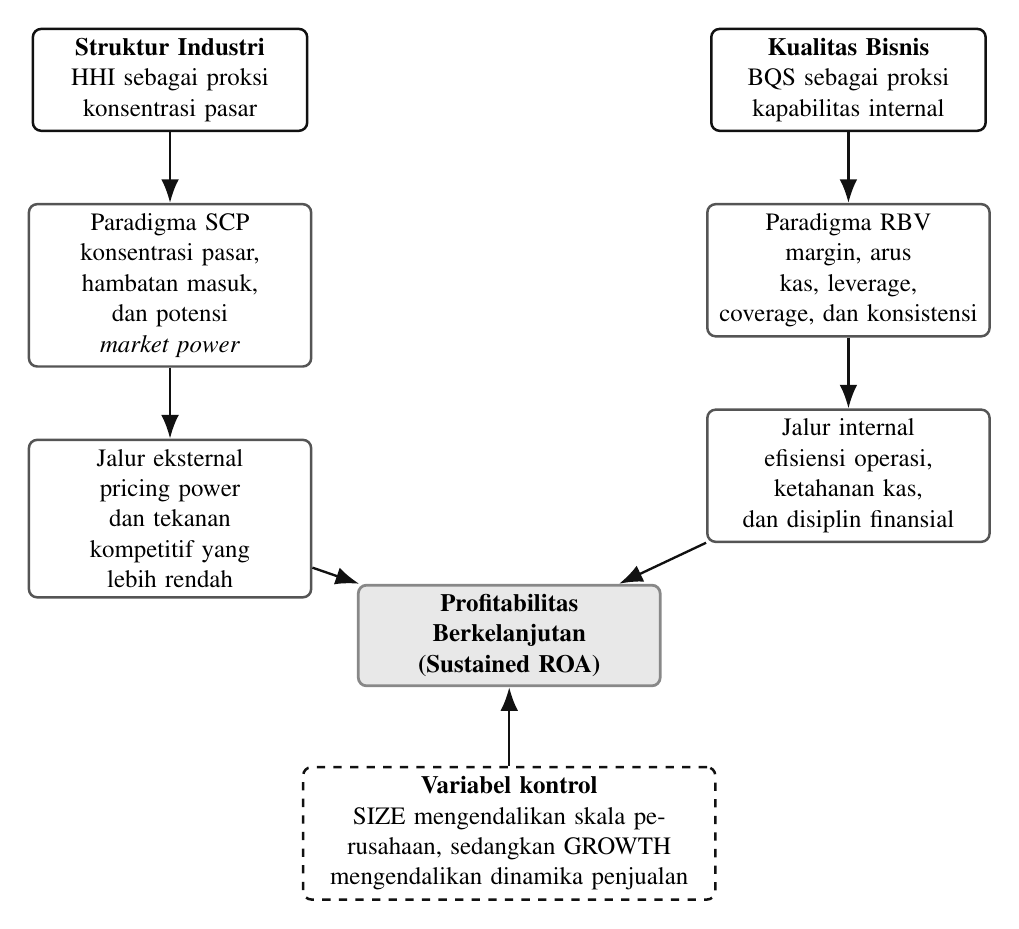
\begin{tikzpicture}[
node distance=0.9cm and 1.1cm,
every node/.style={font=\small, align=center},
mainbox/.style={draw=AksaBlue, rounded corners=3pt, line width=0.9pt, fill=AksaMist, text width=3.25cm, minimum height=1.05cm},
midbox/.style={draw=AksaTeal, rounded corners=3pt, line width=0.9pt, fill=white, text width=3.35cm, minimum height=1cm},
corebox/.style={draw=AksaOrange, rounded corners=3pt, line width=1pt, fill=AksaSand, text width=3.6cm, minimum height=1.15cm},
ctrlbox/.style={draw=AksaBlue, dashed, rounded corners=3pt, line width=0.9pt, fill=white, text width=5.0cm, minimum height=0.95cm},
arrow/.style={-{Latex[length=3mm]}, line width=0.85pt, color=AksaBlue}
]
\node[mainbox] (hhi) {\textbf{Struktur Industri}\\HHI sebagai proksi\\konsentrasi pasar};
\node[mainbox, right=5.1cm of hhi] (bqs) {\textbf{Kualitas Bisnis}\\BQS sebagai proksi\\kapabilitas internal};
\node[midbox, below=of hhi] (scp) {Paradigma SCP\\konsentrasi pasar, hambatan masuk,\\dan potensi \textit{market power}};
\node[midbox, below=of bqs] (rbv) {Paradigma RBV\\margin, arus kas, leverage,\\coverage, dan konsistensi};
\node[midbox, below=of scp] (ext) {Jalur eksternal\\pricing power dan tekanan\\kompetitif yang lebih rendah};
\node[midbox, below=of rbv] (int) {Jalur internal\\efisiensi operasi, ketahanan kas,\\dan disiplin finansial};
\node[corebox, below=1.1cm of $(ext)!0.5!(int)$] (sroa) {\textbf{Profitabilitas Berkelanjutan}\\\textbf{(Sustained ROA)}};
\node[ctrlbox, below=1.0cm of sroa] (ctrl) {\textbf{Variabel kontrol}\\SIZE mengendalikan skala perusahaan, sedangkan GROWTH mengendalikan dinamika penjualan};
\draw[arrow] (hhi) -- (scp);
\draw[arrow] (scp) -- (ext);
\draw[arrow] (ext) -- (sroa);
\draw[arrow] (bqs) -- (rbv);
\draw[arrow] (rbv) -- (int);
\draw[arrow] (int) -- (sroa);
\draw[arrow] (ctrl) -- (sroa);
\end{tikzpicture}
\caption{Kerangka Pemikiran Teoretik Penelitian}
\end{figure}

Gambar 2.1 mendemonstrasikan bahwa tingkat profitabilitas berkelanjutan
(\(SROA_{i,t}\)) tidak terbentuk secara hampa melainkan melalui
transmisi kausalitas teoretis yang jelas. Jalur eksternal (SCP)
menerjemahkan tingkat konsentrasi industri (\(HHI_{j,t}\)) menjadi
keunggulan akibat perlindungan kekuatan pasar dari tekanan persaingan
harga. Jalur internal (RBV) menerjemahkan skor komposit \(BQS_{i,t}\)
menjadi ketahanan operasional, kecukupan likuiditas kas, dan keselamatan
struktural dari risiko insolvensi.

\subsection{Hipotesis Penelitian}\label{hipotesis-penelitian}

Berdasarkan sintesis landasan teoretik dan pembuktian empiris terdahulu,
hipotesis penelitian dirumuskan secara terarah (\emph{directional
hypotheses}) sebagai berikut:

\begin{itemize}
\tightlist
\item
  \textbf{H1}: Tingkat konsentrasi industri (\(HHI_{j,t}\)) berpengaruh
  positif dan signifikan terhadap profitabilitas berkelanjutan
  (\(SROA_{i,t}\)) perusahaan konstituen S\&P 500.
\item
  \textbf{H2}: Kualitas keuangan internal perusahaan (\(BQS_{i,t}\))
  berpengaruh positif dan signifikan terhadap profitabilitas
  berkelanjutan (\(SROA_{i,t}\)) perusahaan konstituen S\&P 500.
\item
  \textbf{H3}: Dalam spesifikasi regresi panel, pengaruh kualitas
  internal (\(BQS_{i,t}\)) bernilai lebih dominan dan memiliki
  konsistensi statistik yang lebih tinggi dalam menjelaskan
  profitabilitas berkelanjutan (\(SROA_{i,t}\)) dibandingkan faktor
  struktur industri eksternal (\(HHI_{j,t}\)).
\item
  \textbf{H4}: Ukuran perusahaan (\(SIZE_{i,t}\)) dan pertumbuhan
  penjualan (\(GROWTH_{i,t}\)) secara simultan berpengaruh signifikan
  sebagai variabel kontrol terhadap profitabilitas berkelanjutan
  (\(SROA_{i,t}\)) emiten.
\end{itemize}

\section{METODE PENELITIAN}\label{metode-penelitian}

Pendekatan penelitian ini berakar pada paradigma positivisme, yang
memandang bahwa realitas ekonomi dapat diobservasi, diukur, dan
dianalisis secara sistematis. Berpijak pada ontologi ini, penelitian
mengadopsi pendekatan kuantitatif deduktif (\emph{hypothetico-deductive
method}) untuk menguji hipotesis yang diturunkan dari paradigma
Structure-Conduct-Performance (SCP) dan Resource-Based View (RBV)
menggunakan data sekunder.

Desain penelitian bersifat eksplanatoris (\emph{explanatory research}),
tetapi klaim yang dihasilkan dibatasi pada hubungan empiris bersyarat
dalam spesifikasi model panel. Dengan kata lain, penelitian ini
bertujuan menjelaskan asosiasi yang konsisten setelah heterogenitas
perusahaan dan guncangan waktu dikendalikan, bukan membuktikan
kausalitas absolut.

\subsection{Variabel Penelitian dan Definisi Operasional
Variabel}\label{variabel-penelitian-dan-definisi-operasional-variabel}

Penelitian ini menggunakan lima variabel utama yang diklasifikasikan ke
dalam tiga kelompok peran: satu variabel dependen, dua variabel
independen utama, dan dua variabel kontrol. Operasionalisasi, formula,
dan justifikasi ilmiah dari setiap variabel diuraikan secara
terintegrasi di bawah ini.

\paragraph{\texorpdfstring{Variabel Dependen: Profitabilitas
Berkelanjutan
(\(SROA_{i,t}\))}{Variabel Dependen: Profitabilitas Berkelanjutan (SROA\_\{i,t\})}}\label{variabel-dependen-profitabilitas-berkelanjutan-sroa_it}

\begin{itemize}
\tightlist
\item
  \textbf{(a) Definisi Konseptual}: Profitabilitas berkelanjutan
  mencerminkan kapabilitas jangka panjang korporasi untuk menghasilkan
  keuntungan ekonomi di atas rata-rata industri secara persisten
  (\emph{abnormal profits} atau \emph{economic rents}). SROA
  merepresentasikan kemampuan adaptasi strategis, efisiensi operasional,
  dan daya tahan parit ekonomi (\emph{economic moat}) perusahaan
  terhadap kekuatan kompetitif pasar yang biasanya mendorong laba
  kembali ke nilai rata-rata (\emph{mean reversion}).
\item
  \textbf{(b) Indikator Pengukuran}: Variabel ini diukur menggunakan
  rata-rata bergerak tiga tahun (\emph{rolling 3-year moving average})
  dari \emph{Return on Assets} (ROA). ROA tahunan diperoleh dari rasio
  laba bersih setelah pajak terhadap total aset: \begin{equation}
  \mathrm{ROA}_{i,t} = \frac{\text{Net Income}_{i,t}}{\text{Total Assets}_{i,t}}
  \end{equation} Kemudian, konstruk SROA dirumuskan secara matematis:
  \begin{equation}
  \mathrm{SROA}_{i,t} = \frac{\mathrm{ROA}_{i,t} + \mathrm{ROA}_{i,t-1} + \mathrm{ROA}_{i,t-2}}{3}
  \end{equation} Di mana \(\mathrm{SROA}_{i,t}\) adalah profitabilitas
  berkelanjutan perusahaan \(i\) pada tahun \(t\).
\item
  \textbf{(c) Alasan Ilmiah Pemilihan}: Penggunaan rata-rata bergerak
  tiga tahun ditujukan untuk mengekstrak komponen laba permanen
  (\emph{sustained earnings}) korporasi dan meredam kebisingan
  transitori (\emph{transitory noise}) dari akrual akuntansi satu tahun
  tunggal, siklus bisnis jangka pendek, atau guncangan industri
  sementara. Hal ini sejalan dengan teori \emph{Persistence of Profit}
  (PoP) dari Dennis Mueller.
\end{itemize}

\paragraph{\texorpdfstring{Variabel Independen Utama: Kualitas Bisnis
(\(BQS_{i,t}\))}{Variabel Independen Utama: Kualitas Bisnis (BQS\_\{i,t\})}}\label{variabel-independen-utama-kualitas-bisnis-bqs_it}

\begin{itemize}
\tightlist
\item
  \textbf{(a) Definisi Konseptual}: Kualitas bisnis internal
  menggambarkan keunggulan kapabilitas keuangan internal yang bersifat
  \emph{valuable, rare, inimitable, and non-substitutable} (VRIN) milik
  perusahaan. Ini merupakan representasi operasional dari mazhab
  \emph{Resource-Based View} (RBV) yang menegaskan bahwa profitabilitas
  unggul berkelanjutan bersumber dari kekuatan sumber daya internal
  korporasi.
\item
  \textbf{(b) Indikator Pengukuran}: BQS dibentuk dari lima komponen
  fundamental keuangan yang bertindak sebagai \textbf{indikator
  formatif} (\emph{formative indicators}):

  \begin{enumerate}
  \def\labelenumi{\arabic{enumi}.}
  \tightlist
  \item
    \emph{Gross Profit Margin} (MARG) sebagai proksi dari kekuatan
    penentuan harga jual (\emph{pricing power}): \begin{equation}
    \mathrm{MARG}_{i,t} = \frac{\text{Sales}_{i,t} - \text{Cost of Goods Sold}_{i,t}}{\text{Sales}_{i,t}}
    \end{equation}
  \item
    \emph{Free Cash Flow Margin} (FCF\_MARGIN) untuk mengukur efisiensi
    konversi laba menjadi kas: \begin{equation}
    \mathrm{FCF\_MARGIN}_{i,t} = \frac{\text{Operating Cash Flow}_{i,t} - \text{Capital Expenditures}_{i,t}}{\text{Sales}_{i,t}}
    \end{equation}
  \item
    Disiplin Leverage Keuangan (LEV) yang dihitung dari komplemen rasio
    utang terhadap aset: \begin{equation}
    \mathrm{LEV}_{i,t} = 1 - \frac{\text{Total Debt}_{i,t}}{\text{Total Assets}_{i,t}}
    \end{equation}
  \item
    Rasio Cakupan Bunga (INTEREST\_COVERAGE) untuk mengukur kapasitas
    proteksi solvabilitas: \begin{equation}
    \mathrm{INTEREST\_COVERAGE}_{i,t} = \frac{\text{Operating Income}_{i,t}}{\text{Interest Expense}_{i,t}}
    \end{equation}
  \item
    Konsistensi Laba (CONS) yang diukur dari kebalikan koefisien variasi
    margin kotor selama tiga tahun: \begin{equation}
    \mathrm{CONS}_{i,t} = \frac{|\mu_{\mathrm{MARG},(t,t-1,t-2)}|}{\sigma_{\mathrm{MARG},(t,t-1,t-2)}}
    \end{equation} Setiap komponen distandarisasi secara tahunan
    menggunakan formula \emph{Z-score} lintas-seksi: \begin{equation}
    Z_{X,i,t} = \frac{X_{i,t} - \mu_{X,t}}{\sigma_{X,t}}
    \end{equation} Skor akhir BQS dirumuskan sebagai rata-rata
    aritmatika berbobot sama dari kelima Z-score komponen:
    \begin{equation}
    \mathrm{BQS}_{i,t} = \frac{Z_{\mathrm{MARG},i,t} + Z_{\mathrm{FCF\_MARGIN},i,t} + Z_{\mathrm{LEV},i,t} + Z_{\mathrm{INTEREST\_COVERAGE},i,t} + Z_{\mathrm{CONS},i,t}}{5}
    \end{equation} Karena pilar finansial penyusun BQS ini bertindak
    sebagai indikator formatif (yang mendefinisikan dimensi kualitas
    internal yang berbeda dan tidak berasumsi adanya kovarians searah),
    pengujian reliabilitas reflektif tradisional seperti
    \emph{Cronbach's Alpha} atau \emph{Composite Reliability} secara
    metodologis \textbf{tidak valid} untuk diterapkan dan tidak boleh
    dipaksakan.
  \end{enumerate}
\item
  \textbf{(c) Alasan Ilmiah Pemilihan}: Indeks komposit ini mencakup
  dimensi profitabilitas, likuiditas, solvabilitas, proteksi bunga, dan
  stabilitas operasional secara terintegrasi. Hal ini memberikan
  evaluasi komprehensif atas parit pertahanan finansial internal
  perusahaan.
\end{itemize}

\paragraph{\texorpdfstring{Variabel Independen Utama: Konsentrasi
Industri
(\(HHI_{j,t}\))}{Variabel Independen Utama: Konsentrasi Industri (HHI\_\{j,t\})}}\label{variabel-independen-utama-konsentrasi-industri-hhi_jt}

\begin{itemize}
\tightlist
\item
  \textbf{(a) Definisi Konseptual}: Konsentrasi pasar merepresentasikan
  hambatan masuk, hambatan persaingan, dan derajat kekuatan
  oligopolistik di pasar eksternal tempat korporasi beroperasi. Ini
  merupakan perwujudan empiris dari mazhab
  \emph{Structure-Conduct-Performance} (SCP) yang berargumen bahwa
  struktur pasar yang terkonsentrasi memfasilitasi koordinasi kolusif
  terselubung dan marjin harga di atas biaya marginal, sehingga
  meningkatkan profitabilitas secara industri.
\item
  \textbf{(b) Indikator Pengukuran}: Diukur menggunakan
  \emph{Herfindahl-Hirschman Index} (HHI) tahunan pada level
  sub-industri GICS (\(j\)) tempat perusahaan \(i\) berada. HHI dihitung
  dengan menjumlahkan kuadrat pangsa pasar (\emph{market share})
  penjualan emiten: \begin{equation}
  \mathrm{HHI}_{j,t} = \sum_{i=1}^{N_j} \left(S_{i,j,t}\right)^2
  \end{equation} Di mana pangsa pasar (\(S_{i,j,t}\)) dihitung
  berdasarkan rasio penjualan individual terhadap total penjualan
  sub-industri: \begin{equation}
  S_{i,j,t} = \frac{\text{Sales}_{i,j,t}}{\sum_{k=1}^{N_j} \text{Sales}_{k,j,t}}
  \end{equation}
\item
  \textbf{(c) Alasan Ilmiah Pemilihan}: HHI merupakan standar emas
  ekonometrika di bidang Organisasi Industri (\emph{Industrial
  Organization}) untuk mengukur tingkat persaingan sektoral. Pengukuran
  HHI pada level sub-industri GICS (\(92\) sub-industri) menawarkan
  tingkat presisi pasar yang sangat tinggi dibandingkan klasifikasi
  industri makro yang terlalu luas.
\end{itemize}

\paragraph{\texorpdfstring{Variabel Kontrol: Ukuran Perusahaan
(\(SIZE_{i,t}\))}{Variabel Kontrol: Ukuran Perusahaan (SIZE\_\{i,t\})}}\label{variabel-kontrol-ukuran-perusahaan-size_it}

\begin{itemize}
\tightlist
\item
  \textbf{(a) Definisi Konseptual}: Ukuran perusahaan mencerminkan skala
  ekonomi (\emph{economies of scale}), kekuatan posisi tawar di pasar
  input-output, serta aksesibilitas ke pasar modal eksternal. Perusahaan
  berskala besar diasumsikan memiliki kestabilan operasi dan risiko
  kebangkrutan yang lebih rendah.
\item
  \textbf{(b) Indikator Pengukuran}: Diproksikan menggunakan logaritma
  natural dari total aset korporasi akhir tahun: \begin{equation}
  \mathrm{SIZE}_{i,t} = \ln(\text{Total Assets}_{i,t})
  \end{equation}
\item
  \textbf{(c) Alasan Ilmiah Pemilihan}: Skala aset emiten raksasa S\&P
  500 memiliki variansi dan kemencengan (\emph{skewness}) ekstrem.
  Penerapan logaritma natural secara ekonometris menekan penyebaran
  nilai ekstrem tersebut guna memastikan model bersifat linier dan
  terhindar dari bias spesifikasi.
\end{itemize}

\paragraph{\texorpdfstring{Variabel Kontrol: Pertumbuhan Penjualan
(\(GROWTH_{i,t}\))}{Variabel Kontrol: Pertumbuhan Penjualan (GROWTH\_\{i,t\})}}\label{variabel-kontrol-pertumbuhan-penjualan-growth_it}

\begin{itemize}
\tightlist
\item
  \textbf{(a) Definisi Konseptual}: Pertumbuhan penjualan
  merepresentasikan tingkat ekspansi bisnis, penerimaan pasar atas
  produk emiten, serta momentum pertumbuhan permintaan industri.
\item
  \textbf{(b) Indikator Pengukuran}: Dihitung dari persentase perubahan
  pendapatan penjualan nominal dari tahun berjalan relatif terhadap
  tahun sebelumnya: \begin{equation}
  \mathrm{GROWTH}_{i,t} = \frac{\text{Sales}_{i,t} - \text{Sales}_{i,t-1}}{\text{Sales}_{i,t-1}}
  \end{equation}
\item
  \textbf{(c) Alasan Ilmiah Pemilihan}: Dimasukkannya GROWTH dirancang
  untuk memisahkan efek siklus peningkatan permintaan dari pengaruh
  kapabilitas internal BQS, sehingga koefisien utama tidak terbiaskan
  oleh fluktuasi siklus penjualan korporasi.
\end{itemize}

\begin{longtable}{>{\raggedright\arraybackslash}p{\dimexpr 0.20\textwidth - 2\tabcolsep} >{\raggedright\arraybackslash}p{\dimexpr 0.10\textwidth - 2\tabcolsep} >{\raggedright\arraybackslash}p{\dimexpr 0.44\textwidth - 2\tabcolsep} >{\raggedright\arraybackslash}p{\dimexpr 0.10\textwidth - 2\tabcolsep} >{\raggedright\arraybackslash}p{\dimexpr 0.16\textwidth - 2\tabcolsep}}
\caption{Ringkasan Definisi Operasional Variabel}\label{tab:definisi-operasional}\\
\toprule
\textbf{Variabel} & \textbf{Simbol} & \textbf{Definisi Operasional} & \textbf{Skala} & \textbf{Sumber Data} \\
\midrule
\endfirsthead
\toprule
\textbf{Variabel} & \textbf{Simbol} & \textbf{Definisi Operasional} & \textbf{Skala} & \textbf{Sumber Data} \\
\midrule
\endhead
Dependen & & & & \\
Profitabilitas Berkelanjutan & SROA & Rata-rata Return on Assets (Laba Bersih / Total Aset) selama 3 tahun (t, t-1, t-2). & Rasio & Bloomberg Terminal \\
Independen & & & & \\
Struktur Industri & HHI & Jumlah kuadrat pangsa pasar penjualan emiten dalam GICS Sub-Industry yang sama ($\sum s_i^2$). & Rasio & Bloomberg Terminal (Kalkulasi) \\
Kualitas Bisnis & BQS & Rata-rata Z-score tahunan dari komponen Margin, FCF Margin, Leverage (komplemen), Interest Coverage, dan Konsistensi laba. & Interval & Bloomberg Terminal (Kalkulasi) \\
Kontrol & & & & \\
Ukuran Perusahaan & SIZE & Logaritma natural dari Total Aset akhir tahun. & Rasio & Bloomberg Terminal \\
Pertumbuhan Penjualan & GROWTH & Persentase perubahan penjualan dari tahun t-1 ke tahun t. & Rasio & Bloomberg Terminal \\
\bottomrule
\end{longtable}

\subsection{Populasi dan Sampel}\label{populasi-dan-sampel}

Uraian mengenai populasi dan penentuan sampel dilakukan secara objektif
dengan bersandar pada prinsip keterwakilan statistik
(\emph{representative sampling}). Populasi target dalam penelitian ini
mencakup seluruh perusahaan besar di Amerika Serikat yang terdaftar
dalam indeks S\&P 500. Dalam pelaksanaan praktis pengambilan sampel,
kerangka sampling yang digunakan adalah seluruh konstituen aktif indeks
S\&P 500 per Mei 2026 yang tersedia di basis data Bloomberg Terminal, di
mana data laporan keuangan historisnya ditarik mundur (\emph{back-cast})
secara tahunan untuk periode pengamatan 2017--2025. Penting untuk diakui
secara transparan sejak awal bahwa metode penarikan data historis secara
longitudinal berdasarkan daftar konstituen aktif pada titik akhir waktu
ini menimbulkan risiko bias kelangsungan hidup (\emph{survivorship
bias}). Emiten yang bangkrut, terlikuidasi, melakukan penggabungan usaha
(\emph{merger}), atau keluar (\emph{delisted}) dari indeks S\&P 500
sebelum Mei 2026 tidak tercakup dalam sampel penelitian. Pengakuan
batasan data eksternal ini bertujuan menjaga integritas akademik hasil
penelitian.

Pengambilan sampel dilakukan menggunakan teknik \emph{Purposive
Sampling} (atau \emph{Judgment Sampling}) dengan menetapkan kriteria
seleksi yang ketat demi meminimalkan bias ekstrinsik. Kriteria seleksi
sampel dirumuskan sebagai berikut: 1. Perusahaan terdaftar secara aktif
sebagai anggota konstituen S\&P 500 per Mei 2026. 2. Perusahaan memiliki
laporan keuangan tahunan yang lengkap pada Bloomberg Terminal selama
periode 2017--2025 (data 2017--2018 digunakan untuk perhitungan variabel
\emph{rolling} dan \emph{lag}, sedangkan panel regresi efektif berjalan
pada periode 2019--2025). 3. Perusahaan tidak tergolong dalam sektor
Keuangan (\emph{Financials} - GICS Code 40) dan sektor Utilitas
(\emph{Utilities} - GICS Code 55). 4. Perusahaan melaporkan kinerja
keuangan dalam mata uang Dolar AS (USD) guna menjamin komparabilitas
rasio keuangan. 5. Perusahaan memiliki data lengkap untuk pembentukan
seluruh komponen indeks BQS komposit (\emph{complete-case policy}).

Kebijakan eksklusi sektoral secara khusus diterapkan terhadap sektor
Keuangan dan Utilitas berdasarkan pembenaran ilmiah (\emph{justifikasi
ilmiah}) yang sangat kuat. Pertama, sektor Keuangan didepan karena
emiten perbankan dan lembaga keuangan memiliki struktur neraca dan pola
operasional yang berbeda secara fundamental dari sektor industri
non-keuangan. Bagi perusahaan keuangan, dana pihak ketiga
(deposito/utang) bertindak sebagai bahan baku operasional utama yang
disalurkan kembali dalam bentuk kredit, bukan sebagai sumber leverage
pendanaan tambahan. Akibatnya, rasio leverage keuangan dan margin kotor
mereka tidak sebanding secara \emph{apple-to-apple} dengan sektor
lainnya. Memasukkan sektor keuangan akan merusak validitas pembentukan
komponen LEV dan MARG dalam indeks BQS. Kedua, sektor Utilitas
dikeluarkan karena emiten utilitas beroperasi di bawah payung monopoli
alamiah yang diregulasi secara ketat (\emph{regulated monopolies}).
Tingkat profitabilitas dan penentuan harga jual mereka didikte oleh
batas atas tarif yang ditetapkan regulator (\emph{regulatory
rate-of-return regulation}), bukan oleh efisiensi murni operasional
internal atau persaingan pasar bebas. Penyatuan sektor utilitas akan
membingungkan analisis pengaruh variabel BQS dan HHI terhadap SROA.

Untuk menangani keberadaan nilai pencilan (\emph{outliers}) ekstrem yang
lazim ditemui dalam data rasio keuangan korporat (akibat
restrukturisasi, penghapusan nilai aset luar biasa, atau pembagian
dengan angka mendekati nol), penelitian ini menerapkan teknik
\textbf{Winsorization} pada tingkat persentil 1\% dan 99\% di kedua ekor
distribusi variabel rasio kontinu utama (SROA, BQS components, dan
GROWTH). Melalui Winsorization, nilai data di bawah persentil ke-1 akan
diganti dengan nilai ambang batas persentil ke-1, dan nilai data di atas
persentil ke-99 akan diganti dengan nilai ambang batas persentil ke-99.
Teknik ini secara ekonometris sangat superior dibandingkan dengan
pemotongan data (\emph{trimming}) karena mampu menjinakkan distorsi
pencilan tanpa mengurangi jumlah baris observasi panel final, sehingga
jumlah sampel tetap terjaga secara konsisten pada \(N = 2241\) observasi
dari 333 perusahaan selama periode panel efektif 2019--2025.

\subsection{Jenis dan Sumber Data}\label{jenis-dan-sumber-data}

Penelitian ini menggunakan jenis data sekunder kuantitatif yang disusun
dalam bentuk struktur \textbf{Data Panel (Longitudinal Data)}. Data
panel mengintegrasikan dimensi lintas-seksi (\emph{cross-section})
sebanyak 333 perusahaan dengan dimensi deret waktu (\emph{time-series})
tahunan selama periode panel efektif 2019--2025. Secara metodologis,
penggunaan data panel memberikan keunggulan kritis dibandingkan data
lintas-seksi tunggal atau deret waktu murni. Keunggulan utamanya adalah
kemampuan struktur panel untuk mendeteksi dan mengontrol heterogenitas
tidak teramati (\emph{unobserved heterogeneity})---karakteristik laten
spesifik perusahaan yang konstan sepanjang waktu (seperti reputasi
merek, kapabilitas manajerial, kultur organisasi, dan strategi
korporasi) namun berbeda antar-firma. Mengabaikan faktor heterogenitas
laten ini akan memicu masalah bias variabel yang terlewat (\emph{omitted
variable bias}), yang menyebabkan estimator parameter regresi menjadi
bias dan tidak konsisten. Selain itu, data panel meningkatkan derajat
kebebasan (\emph{degrees of freedom}) dan meminimalkan masalah
kolinearitas antar variabel independen.

Sumber data sekunder dalam penelitian ini seluruhnya diperoleh secara
digital dari \textbf{Bloomberg Terminal} yang memiliki reputasi
kredibilitas tinggi di kalangan akademisi keuangan global. Item data
yang diunduh mencakup angka laporan keuangan tahunan seperti total aset,
penjualan nominal, laba bersih, arus kas operasi, belanja modal (Capex),
total utang, harga pokok penjualan (COGS), laba operasi, dan beban
bunga. Klasifikasi industri emiten bersumber dari pengelompokan resmi
\emph{Industry Classification Benchmark} (ICB) dan \emph{Global Industry
Classification Standard} (GICS) guna menentukan batas pasar dalam
penghitungan HHI.

Untuk memberikan gambaran ringkas dan terintegrasi mengenai seluruh
variabel, jenis data, dan sumber pengambilannya, Tabel 3.1 berikut
merangkum operasionalisasi variabel secara sistematis.

\begin{longtable}{>{\raggedright\arraybackslash}p{\dimexpr 0.20\textwidth - 2\tabcolsep} >{\raggedright\arraybackslash}p{\dimexpr 0.10\textwidth - 2\tabcolsep} >{\raggedright\arraybackslash}p{\dimexpr 0.44\textwidth - 2\tabcolsep} >{\raggedright\arraybackslash}p{\dimexpr 0.10\textwidth - 2\tabcolsep} >{\raggedright\arraybackslash}p{\dimexpr 0.16\textwidth - 2\tabcolsep}}
\caption{Ringkasan Definisi Operasional Variabel}\label{tab:definisi-operasional}\\
\toprule
\textbf{Variabel} & \textbf{Simbol} & \textbf{Definisi Operasional} & \textbf{Skala} & \textbf{Sumber Data} \\
\midrule
\endfirsthead
\toprule
\textbf{Variabel} & \textbf{Simbol} & \textbf{Definisi Operasional} & \textbf{Skala} & \textbf{Sumber Data} \\
\midrule
\endhead
Dependen & & & & \\
Profitabilitas Berkelanjutan & SROA & Rata-rata Return on Assets (Laba Bersih / Total Aset) selama 3 tahun (t, t-1, t-2). & Rasio & Bloomberg Terminal \\
Independen & & & & \\
Struktur Industri & HHI & Jumlah kuadrat pangsa pasar penjualan emiten dalam GICS Sub-Industry yang sama ($\sum s_i^2$). & Rasio & Bloomberg Terminal (Kalkulasi) \\
Kualitas Bisnis & BQS & Rata-rata Z-score tahunan dari komponen Margin, FCF Margin, Leverage (komplemen), Interest Coverage, dan Konsistensi laba. & Interval & Bloomberg Terminal (Kalkulasi) \\
Kontrol & & & & \\
Ukuran Perusahaan & SIZE & Logaritma natural dari Total Aset akhir tahun. & Rasio & Bloomberg Terminal \\
Pertumbuhan Penjualan & GROWTH & Persentase perubahan penjualan dari tahun t-1 ke tahun t. & Rasio & Bloomberg Terminal \\
\bottomrule
\end{longtable}

\subsection{Metode Pengumpulan Data}\label{metode-pengumpulan-data}

Pengumpulan data dilakukan menggunakan teknik dokumentasi dan arsip
elektronik secara sistematis. Protokol ekstraksi data dirancang secara
ketat untuk menjamin replikasi dan auditabilitas penelitian: 1.
Ekstraksi data mentah laporan keuangan tahunan periode 2017--2025 untuk
konstituen aktif S\&P 500 per Mei 2026 diunduh dari basis data Bloomberg
Terminal ke dalam format berkas comma-separated values
(\texttt{raw-data.csv}). 2. Melakukan audit kebersihan data
(\emph{missingness audit}) untuk mengidentifikasi keberadaan sel kosong
atau anomali data (ambiguous suffix). Sel data yang hilang atau cacat
pada variabel-variabel utama diidentifikasi secara cermat. 3. Menerapkan
kebijakan pembersihan data berbasis kasus lengkap (\textbf{complete-case
policy}). Observasi tahun-perusahaan yang kehilangan data pada salah
satu dari lima pilar komponen BQS utama langsung dikeluarkan dari sampel
regresi utama. Kebijakan ini diambil demi menjaga keandalan dan
integritas pengujian empiris tanpa harus melakukan rekayasa imputasi
statistik buatan yang tidak dapat diverifikasi secara riil. 4.
Menghitung variabel komposit BQS dan HHI tahunan menggunakan skrip
otomasi Python, dilanjutkan dengan penerapan Winsorization pada
persentil 1\% dan 99\%. Dataset panel final disimpan dalam format
\emph{long-form} siap olah.

\subsection{Metode Analisis}\label{metode-analisis}

Tahapan analisis data kuantitatif panel dilakukan secara hierarkis
menggunakan bahasa pemrograman Python dengan pustaka ilmiah
\texttt{pandas}, \texttt{statsmodels}, dan \texttt{linearmodels} untuk
menghasilkan parameter estimasi yang akurat dan stabil.

\subsubsection{Deskripsi Statistik
Model}\label{deskripsi-statistik-model}

Analisis deskriptif digunakan untuk memberikan gambaran umum mengenai
profil numerik distribusi seluruh variabel penelitian. Parameter
statistik tendensi sentral yang dihitung meliputi rata-rata aritmatika
(\(\mu\)): \begin{equation}
\mu = \frac{1}{N \cdot T} \sum_{i=1}^N \sum_{t=1}^T X_{i,t}
\end{equation} Median, yaitu nilai tengah data ketika diurutkan dari
yang terkecil ke terbesar. Dispersi data diukur menggunakan standar
deviasi (\(\sigma\)): \begin{equation}
\sigma = \sqrt{\frac{1}{N \cdot T - 1} \sum_{i=1}^N \sum_{t=1}^T (X_{i,t} - \mu)^2}
\end{equation} Serta varians (\(\sigma^2\)), kuartil pertama (\(Q_1\)),
kuartil ketiga (\(Q_3\)), nilai minimum, dan nilai maksimum. Guna
melihat pola hubungan bivariat awal antar-variabel independen dan
mendeteksi indikasi awal multikolinearitas, dibangun matriks korelasi
linear Pearson (\emph{Pearson Correlation matrix}).

Selain pengujian deskriptif parametrik, dilakukan analisis
non-parametrik dengan membagi sampel ke dalam kelompok desil untuk
variabel BQS (\(D_1\) hingga \(D_{10}\)) dan kuintil untuk variabel HHI
(\(Q_1\) hingga \(Q_5\)). Rata-rata SROA pada tiap kelompok desil BQS
dan kuintil HHI dihitung secara lintas-seksi untuk mengamati profil
kelima komponen fundamental pendukungnya dan mendeteksi pola asosiasi
non-linear atau monotonik awal sebelum model regresi panel formal
diestimasi.

\subsubsection{Pemilihan Spesifikasi
Model}\label{pemilihan-spesifikasi-model}

Pemilihan model estimasi data panel terbaik dilakukan secara formal
dengan membandingkan tiga metode estimator kandidat: \emph{Common Effect
Model} (CEM atau Pooled OLS), \emph{Random Effect Model} (REM), dan
\emph{Fixed Effect Model} (FEM). Alur pengujian formal dilakukan melalui
tiga tahapan uji statistik berikut:

\begin{enumerate}
\def\labelenumi{\arabic{enumi}.}
\item
  \textbf{Uji Chow (Restricted F-Test)}: Digunakan untuk membandingkan
  model CEM dengan FEM. Rumus statistik uji Chow diformulasikan sebagai:
  \begin{equation}
  F = \frac{(\mathrm{RRSS} - \mathrm{URSS}) / (N - 1)}{\mathrm{URSS} / (N \cdot T - N - K)}
  \end{equation} Di mana \(\mathrm{RRSS}\) melambangkan \emph{Residual
  Sum of Squares} yang dibatasi (dari model CEM), \(\mathrm{URSS}\)
  melambangkan \emph{Residual Sum of Squares} yang tidak dibatasi (dari
  model FEM), \(N\) adalah jumlah perusahaan, \(T\) adalah jumlah
  periode waktu, dan \(K\) adalah jumlah variabel penjelas. Hipotesis
  nol menyatakan bahwa intersep untuk seluruh perusahaan adalah sama
  (CEM terpilih).
\item
  \textbf{Uji Breusch-Pagan Lagrange Multiplier (LM)}: Digunakan untuk
  membandingkan model CEM dengan REM. Rumus statistik uji LM dirumuskan
  sebagai: \begin{equation}
  \mathrm{LM} = \frac{N \cdot T}{2(T - 1)} \left[ \frac{\sum_{i=1}^N \left( \sum_{t=1}^T \hat{e}_{i,t} \right)^2}{\sum_{i=1}^N \sum_{t=1}^T \hat{e}_{i,t}^2} - 1 \right]^2 \sim \chi^2(1)
  \end{equation} Di mana \(\hat{e}_{i,t}\) adalah residual dari estimasi
  Pooled OLS (CEM). Hipotesis nol menyatakan varians efek spesifik
  individu adalah nol (CEM terpilih).
\item
  \textbf{Uji Spesifikasi Hausman}: Digunakan untuk membandingkan model
  REM dengan FEM. Rumus statistik uji Hausman (\(H\)) diformulasikan
  sebagai: \begin{equation}
  H = (\hat{\beta}_{\mathrm{FE}} - \hat{\beta}_{\mathrm{RE}})' \left[ \hat{V}(\hat{\beta}_{\mathrm{FE}}) - \hat{V}(\hat{\beta}_{\mathrm{RE}}) \right]^{-1} (\hat{\beta}_{\mathrm{FE}} - \hat{\beta}_{\mathrm{RE}}) \sim \chi^2(K)
  \end{equation} Di mana \(\hat{\beta}_{\mathrm{FE}}\) dan
  \(\hat{\beta}_{\mathrm{RE}}\) adalah vektor koefisien parameter
  berdimensi \(K \times 1\) hasil estimasi model FEM dan REM, sedangkan
  \(\hat{V}(\hat{\beta}_{\mathrm{FE}})\) dan
  \(\hat{V}(\hat{\beta}_{\mathrm{RE}})\) adalah matriks
  varians-kovarians dari kedua estimator tersebut. Hipotesis nol
  menyatakan bahwa efek spesifik individu tidak berkorelasi dengan
  regressor (REM efisien dan konsisten).
\end{enumerate}

Secara teoretis, dalam analisis data keuangan korporat lintas tahun,
model \emph{Fixed Effects} (FEM) hampir selalu jauh lebih konsisten
dibandingkan model \emph{Random Effects} (REM). Hal ini disebabkan
karena karakteristik internal perusahaan yang tidak terobservasi
(seperti strategi bisnis, reputasi merek, kualitas manajerial, kultur
korporasi) hampir pasti berkorelasi secara dinamis dengan keputusan
keuangan dan kapabilitas internal perusahaan (variabel BQS, SIZE, maupun
GROWTH). Oleh karena itu, pengujian Hausman berfungsi sebagai verifikasi
statistik pelengkap, sedangkan FEM tetap menjadi pilihan yang secara
desain teoretis lebih defensibel. Lebih lanjut, dilakukan pengujian efek
waktu (\emph{poolability test} untuk year dummy) untuk menentukan
signifikansi masuknya efek tetap waktu tahunan (\emph{year fixed
effects}). Jika signifikansi terbukti, maka spesifikasi terpilih adalah
\textbf{Two-way Fixed Effects Model (Two-way FEM)} untuk mengendalikan
efek individu perusahaan sekaligus guncangan makro tahunan.

\subsubsection{Estimasi Parameter Model}\label{estimasi-parameter-model}

Model regresi panel utama diestimasi menggunakan spesifikasi formal
model \emph{Two-way Fixed Effects} (Two-way FEM). Model matematis
dirumuskan sebagai berikut: \begin{equation}
\mathrm{SROA}_{i,t} = \beta_0 + \beta_1\,\mathrm{BQS}_{i,t} + \beta_2\,\mathrm{HHI}_{j,t} + \beta_3\,\mathrm{SIZE}_{i,t} + \beta_4\,\mathrm{GROWTH}_{i,t} + \alpha_i + \delta_t + \varepsilon_{i,t}
\end{equation} Di mana \(\alpha_i\) melambangkan efek tetap
karakteristik spesifik individu perusahaan \(i\) yang konstan sepanjang
waktu (\emph{firm fixed effects}), sedangkan \(\delta_t\) melambangkan
efek tetap waktu tahun \(t\) yang mewakili guncangan makroekonomi
tahunan (\emph{year fixed effects}).

Untuk mengestimasi koefisien \(\beta\) secara konsisten dan
mengeliminasi efek tetap individu (\(\alpha_i\)) serta efek tetap waktu
(\(\delta_t\)), dilakukan prosedur transformasi de-meaning dua arah
(\emph{Within Transformation}): \begin{equation}
\ddot{Y}_{i,t} = Y_{i,t} - \bar{Y}_i - \bar{Y}_t + \bar{Y}
\end{equation} \begin{equation}
\ddot{X}_{i,t} = X_{i,t} - \bar{X}_i - \bar{X}_t + \bar{X}
\end{equation} Di mana \(\bar{Y}_i\) dan \(\bar{X}_i\) adalah rata-rata
perusahaan lintas waktu, \(\bar{Y}_t\) dan \(\bar{X}_t\) adalah
rata-rata periode lintas perusahaan, and \(\bar{Y}\) serta \(\bar{X}\)
adalah rata-rata keseluruhan data (\emph{grand mean}). Model estimasi
setelah transformasi dirumuskan sebagai: \begin{equation}
\ddot{Y}_{i,t} = \beta \ddot{X}_{i,t} + \ddot{\epsilon}_{i,t}
\end{equation} Estimator OLS kemudian diterapkan pada data yang telah
ditransformasikan tersebut untuk menghasilkan estimasi
\(\hat{\beta}_{\mathrm{FE}}\) yang bebas bias heterogenitas konstan.

\subsubsection{Diagnostik Asumsi Model}\label{diagnostik-asumsi-model}

Untuk mengevaluasi kelayakan model estimasi panel terhadap asumsi
Gauss-Markov yang disesuaikan untuk model data panel, dilakukan
serangkaian pengujian diagnostik residual:

\begin{enumerate}
\def\labelenumi{\arabic{enumi}.}
\item
  \textbf{Uji Jarque-Bera (Normalitas Residual)}: Menguji apakah
  residual model berdistribusi normal dengan rumus: \begin{equation}
  \mathrm{JB} = \frac{n}{6} \left[ S^2 + \frac{(K - 3)^2}{4} \right]
  \end{equation} Di mana \(n\) adalah jumlah observasi, \(S\) adalah
  skewness residual, dan \(K\) adalah kurtosis residual. Hipotesis nol
  menyatakan residual berdistribusi normal.
\item
  \textbf{Uji Heteroskedastisitas Breusch-Pagan}: Menguji apakah varians
  residual bersifat tidak konstan lintas observasi: \begin{equation}
  \sigma_{i,t}^2 = \sigma^2 f(\gamma' Z_{i,t})
  \end{equation} Di mana \(Z_{i,t}\) adalah vektor variabel penjelas.
  Hipotesis nol menyatakan residual bersifat homoskedastik.
\item
  \textbf{Uji CD Pesaran (Dependensi Lintas-Seksi)}: Memeriksa korelasi
  residual antar-perusahaan lintas-seksi pada tahun pengamatan yang
  sama: \begin{equation}
  \mathrm{CD} = \sqrt{\frac{2T}{N(N - 1)}} \left( \sum_{i=1}^{N-1} \sum_{j=i+1}^N \hat{\rho}_{i,j} \right)
  \end{equation} Di mana \(\hat{\rho}_{i,j}\) adalah nilai korelasi
  berpasangan antara residual perusahaan \(i\) dan \(j\). Hipotesis nol
  menyatakan tidak terdapat dependensi lintas-seksi.
\item
  \textbf{Uji Autokorelasi Serial (\emph{Within-firm} AR(1))}: Mengingat
  panel data penelitian ini berdimensi \(N\)-dominan dengan rentang
  waktu relatif pendek (\(T = 7\)), pendekatan yang paling relevan untuk
  mendeteksi autokorelasi serial bukan melalui uji Durbin-Watson klasik
  (yang dirancang untuk data deret waktu tunggal), melainkan melalui
  kalkulasi langsung koefisien autokorelasi orde pertama dari residual
  \emph{within-transformation}. Koefisien korelasi AR(1) rata-rata
  dihitung sebagai: \begin{equation}
  \hat{\rho}_{\mathrm{AR}(1),i} = \frac{\sum_{t=2}^{T} \ddot{e}_{i,t} \cdot \ddot{e}_{i,t-1}}{\sum_{t=2}^{T} \ddot{e}_{i,t-1}^2}
  \end{equation} Di mana \(\ddot{e}_{i,t}\) adalah residual
  \emph{within-demeaned} perusahaan \(i\) pada tahun \(t\). Nilai
  \(\bar{\hat{\rho}}_{\mathrm{AR}(1)}\) yang signifikan secara statistik
  mendekati atau melebihi 0,5 mengindikasikan autokorelasi serial yang
  kuat dan signifikan, yang merupakan fenomena alamiah pada data
  keuangan korporasi tahunan. Keberadaan autokorelasi serial ini tidak
  mendiskualifikasi estimator Fixed Effects, melainkan menjadi
  justifikasi untuk penerapan koreksi \emph{Firm-Clustered Robust
  Standard Errors} pada tahapan selanjutnya.
\end{enumerate}

\subsubsection{Koreksi Ketahanan Model}\label{koreksi-ketahanan-model}

Apabila hasil uji diagnostik menunjukkan adanya pelanggaran asumsi
heteroskedastisitas dan autokorelasi serial residual (yang sangat lazim
terjadi pada data panel keuangan korporasi karena kinerja keuangan
secara alamiah persisten dari tahun ke tahun), maka standard error biasa
dari OLS akan bias ke bawah secara artifisial. Hal ini menyebabkan nilai
t-statistik menjadi terlalu besar secara semu
(\emph{over-significance}). Guna mengoreksi bias ini secara mutlak,
standard error diestimasi menggunakan metode \textbf{Firm-Clustered
Robust Standard Errors (Petersen, 2009)}. Rumus matriks
varians-kovarians robust diformulasikan sebagai: \begin{equation}
V_{\mathrm{clustered}} = (X'X)^{-1} \left( \sum_{i=1}^N X_i' \hat{\epsilon}_i \hat{\epsilon}_i' X_i \right) (X'X)^{-1}
\end{equation} Di mana \(X_i\) adalah matriks variabel penjelas untuk
perusahaan \(i\), dan \(\hat{\epsilon}_i\) adalah vektor residual
perusahaan \(i\) lintas waktu. Pendekatan ekonometrika ini melonggarkan
asumsi independensi residual murni (\emph{i.i.d}) dan mengizinkan adanya
autokorelasi serial lintas-periode di dalam klaster perusahaan yang sama
dan heteroskedastisitas antar-perusahaan, sehingga menghasilkan standard
error yang robust, konservatif, dan p-value yang valid untuk penarikan
keputusan hipotesis.

Selanjutnya, rencana uji ketahanan model dirancang melalui tiga jalur
spesifikasi alternatif berikut: 1. \textbf{Uji Ketahanan Proksi
Independen Utama}: Mengestimasi model dengan mengganti variabel BQS
utama dengan variabel BQS \emph{legacy} versi 4 komponen (tanpa komponen
konsistensi laba). 2. \textbf{Uji Ketahanan Batas Pasar Industri}:
Mengukur sensitivitas variabel HHI dengan mengestimasi model menggunakan
taksonomi industri alternatif yang lebih lebar (ICB Subsector, ICB
Sector, ICB Industry, dan Bloomberg Industry Group). 3. \textbf{Uji
Ketahanan Outcome Profitabilitas}: Mengestimasi model regresi dengan
mengganti variabel dependen SROA dengan \emph{Sustained Return on
Equity} (SROE) sebagai proksi profitabilitas pemegang saham
berkelanjutan.

\subsubsection{Pengujian Signifikansi
Model}\label{pengujian-signifikansi-model}

Penarikan keputusan inferensial terhadap hipotesis yang diajukan
bersandar pada kriteria keputusan statistik formal berikut:

\begin{enumerate}
\def\labelenumi{\arabic{enumi}.}
\item
  \textbf{Uji Signifikansi Parsial (Uji t)}: Digunakan untuk menguji
  apakah secara individual variabel independen utama (\(BQS\), \(HHI\))
  dan kontrol (\(SIZE\), \(GROWTH\)) memiliki pengaruh nyata terhadap
  profitabilitas berkelanjutan (\(SROA\)). Mengingat arah pengaruh
  hipotesis pada BAB II telah ditentukan secara apriori berdasarkan
  kerangka teori ekonomi keuangan, pengujian dilakukan menggunakan
  \textbf{Uji Satu Arah (\emph{One-tailed Test})}. Nilai statistik uji
  \(t\) dihitung menggunakan formula ekonometrika berikut:
  \begin{equation}
  t = \frac{\hat{\beta}_k}{\mathrm{se}(\hat{\beta}_k)}
  \end{equation} Di mana \(\hat{\beta}_k\) melambangkan nilai estimasi
  koefisien parameter untuk variabel independen ke-\(k\), dan
  \(\mathrm{se}(\hat{\beta}_k)\) melambangkan standard error robust yang
  diklaster pada tingkat perusahaan (\emph{firm-clustered robust
  standard error}). Arah pengujian satu arah yang digunakan adalah:

  \begin{itemize}
  \tightlist
  \item
    Pengujian satu arah kanan (\emph{right-tailed test}) untuk variabel
    BQS, HHI, dan SIZE, dengan hipotesis alternatif menyatakan koefisien
    bernilai positif lebih besar dari nol (\(H_a: \beta_k > 0\)).
  \item
    Pengujian satu arah kiri (\emph{left-tailed test}) untuk variabel
    GROWTH, dengan hipotesis alternatif menyatakan koefisien bernilai
    negatif kurang dari nol (\(H_a: \beta_k < 0\)). Keputusan penolakan
    hipotesis nol (\(H_0\)) diambil jika nilai statistik \(t\)-hitung
    melebihi nilai kritis distribusi \(t\) pada derajat kebebasan
    terkait, atau jika nilai \(p\)-value berada di bawah ambang batas
    signifikansi yang ditentukan (\(\alpha = 0,05\) atau
    \(\alpha = 0,10\)).
  \end{itemize}
\item
  \textbf{Uji Signifikansi Simultan (Uji F)}: Digunakan untuk menguji
  apakah seluruh variabel penjelas (\(BQS\), \(HHI\), \(SIZE\),
  \(GROWTH\)) secara simultan (bersama-sama) memiliki pengaruh yang
  signifikan terhadap \(SROA\). Nilai statistik uji \(F\) untuk
  pembatasan linier seluruh parameter secara serentak diformulasikan
  sebagai berikut: \begin{equation}
  F = \frac{R^2 / K}{(1 - R^2) / (N \cdot T - K - 1)}
  \end{equation} Di mana \(R^2\) melambangkan koefisien determinasi
  model, \(K\) melambangkan jumlah variabel independen dalam model
  regresi (dalam penelitian ini \(K = 4\)), \(N\) melambangkan jumlah
  unit lintas-seksi (perusahaan), dan \(T\) melambangkan jumlah periode
  deret waktu. Hipotesis nol menyatakan bahwa seluruh koefisien
  parameter bernilai nol secara serentak
  (\(H_0: \beta_1 = \beta_2 = \beta_3 = \beta_4 = 0\)). Hipotesis nol
  ditolak jika nilai \(p\)-value dari F-hitung berada di bawah
  \(\alpha = 0,05\).
\item
  \textbf{Koefisien Determinasi (\(R^2\) Within)}: Digunakan untuk
  mengukur daya penjelas model dalam menjelaskan variansi internal
  variabel dependen (\(SROA\)) sepanjang periode pengamatan setelah
  mengeliminasi efek tetap perusahaan dan efek tetap tahunan. \(R^2\)
  Within diformulasikan sebagai: \begin{equation}
  R^2_{\mathrm{within}} = 1 - \frac{\sum_{i=1}^N \sum_{t=1}^T \ddot{e}_{i,t}^2}{\sum_{i=1}^N \sum_{t=1}^T \ddot{y}_{i,t}^2}
  \end{equation} Di mana \(\ddot{e}_{i,t}\) melambangkan residual yang
  telah ditransformasikan de-meaning dua arah, dan \(\ddot{y}_{i,t}\)
  melambangkan variabel dependen \(SROA\) yang dide-mean. Nilai
  \(R^2_{\mathrm{within}}\) berkisar antara 0 hingga 1, menggambarkan
  proporsi variasi profitabilitas berkelanjutan \emph{within-firm} yang
  mampu dijelaskan oleh variasi variabel-variabel penjelas dalam model
  regresi. hipotesis penelitian.
\end{enumerate}

\section{HASIL DAN ANALISIS}\label{hasil-dan-analisis}

BAB IV menyajikan temuan empiris dari pengolahan data Bloomberg Terminal
untuk perusahaan konstituen S\&P 500 aktif per Mei 2026. Uraian pada bab
ini difokuskan pada hasil olah data, kelayakan model, pengujian
hipotesis, dan interpretasi ekonomi. Definisi variabel, rumus, teknik
estimasi, serta prosedur konstruksi BQS dan HHI telah dijelaskan pada
BAB III sehingga tidak diulang secara panjang pada bab ini. Visualisasi
Python lengkap ditempatkan pada lampiran sebagai dokumentasi audit;
visual dalam BAB IV disajikan dalam bentuk rangkuman yang dikurasi agar
pembacaan hasil tetap ringkas.

\subsection{Deskripsi Variabel
Penelitian}\label{deskripsi-variabel-penelitian}

Bagian ini menyajikan karakteristik empiris dan perilaku distribusi dari
setiap variabel yang digunakan dalam model panel. Berbeda dengan
deskripsi statistik formal pada § 4.2.1, uraian pada bagian ini bersifat
kontekstual dan interpretatif: mengurai profil setiap variabel secara
mendalam berdasarkan konstruksi, distribusi, dan dinamika waktunya,
serta menyertakan visualisasi distribusi guna memberikan kesan intuitif
yang kuat sebelum masuk ke pengujian ekonometrika. Analisis ini mencakup
keempat variabel utama model regresi panel: satu variabel dependen
(SROA), dua variabel independen (BQS dan HHI), dan dua variabel kontrol
(SIZE dan GROWTH).

\subsubsection{Variabel Dependen: SROA}\label{variabel-dependen-sroa}

Variabel dependen penelitian ini adalah \emph{Sustained Return on
Assets} (SROA), yang didefinisikan sebagai rata-rata bergerak tiga tahun
dari rasio laba bersih terhadap total aset. Konstruksi melalui rata-rata
bergerak (\emph{rolling average}) dilakukan secara disengaja untuk
menyaring komponen profitabilitas yang bersifat permanen dan struktural,
sekaligus mereduksi kebisingan transitori dari guncangan satu tahun yang
tidak representatif terhadap kapabilitas jangka panjang perusahaan.
Dalam konteks teori \emph{Persistence of Profit} (Mueller, 1977), SROA
merepresentasikan kemampuan suatu korporasi untuk mempertahankan
keunggulan laba di atas rata-rata industri secara berkelanjutan, suatu
properti yang hanya dapat dicapai oleh perusahaan yang memiliki
keunggulan kompetitif struktural yang riil.

Distribusi SROA di seluruh 2.241 observasi panel (333 perusahaan
\(\times\) 7 tahun) mencatat nilai rata-rata sebesar \textbf{0,079
(7,9\%)} dengan nilai median sebesar \textbf{0,070 (7,0\%)}. Perbedaan
antara rata-rata dan median yang sebesar 0,9 persentase poin
mengindikasikan distribusi yang sedikit menceng ke kanan
(\emph{right-skewed}), yaitu terdapat sekelompok kecil perusahaan dengan
SROA yang sangat tinggi yang menarik rata-rata ke atas. Nilai minimum
distribusi menyentuh -0,095 (-9,5\%), sementara nilai maksimumnya
mencapai 0,276 (27,6\%). Rentang yang lebar ini---sebesar 37,1
persentase poin---membuktikan adanya heterogenitas profitabilitas
berkelanjutan yang sangat dramatis dan asimetris di antara
perusahaan-perusahaan besar konstituen S\&P 500, bahkan setelah perataan
melalui rata-rata bergerak tiga tahun.

Gambar 4.1 memvisualisasikan distribusi SROA dalam bentuk histogram
distribusi dan \emph{box-plot} perbandingan lintas-sektor,
mengilustrasikan pola kemencengan distribusi sekaligus rentang
antar-kuartil yang sangat luas sebagai bukti visual heterogenitas
profitabilitas korporasi.

\begin{figure}[H]
\caption{Distribusi dan Perilaku SROA: Histogram Kemencengan}
\centering
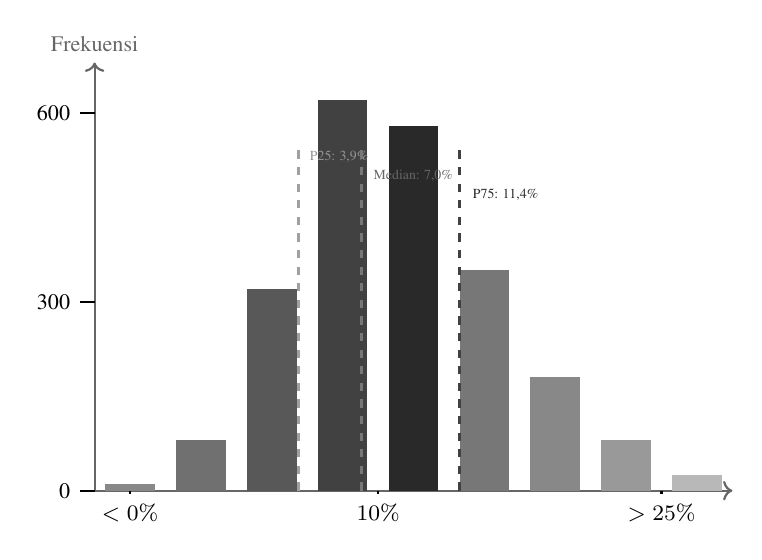
\begin{tikzpicture}[x=0.9cm, y=0.008cm]
% Draw axes
\draw[->, thick, black!60] (-0.5, 0) -- (8.5, 0);
\draw[->, thick, black!60] (-0.5, 0) -- (-0.5, 680) node[above, font=\footnotesize] {Frekuensi};

% Axis ticks Sumbu X - only left, center, right to avoid overlap
\draw[thick] (0, 0) -- (0, -5) node[below, font=\footnotesize] {$<0\%$};
\draw[thick] (3.5, 0) -- (3.5, -5) node[below, font=\footnotesize] {$10\%$};
\draw[thick] (7.5, 0) -- (7.5, -5) node[below, font=\footnotesize] {$>25\%$};

% Axis ticks Sumbu Y - only key numbers
\draw[thick] (-0.5, 0) -- (-0.7, 0) node[left, font=\footnotesize] {0};
\draw[thick] (-0.5, 300) -- (-0.7, 300) node[left, font=\footnotesize] {300};
\draw[thick] (-0.5, 600) -- (-0.7, 600) node[left, font=\footnotesize] {600};

% Bars - simple, neat, consistent width and spacing
\foreach \x/\h/\col in {
  0/10/AksaBlue!50,
  1/80/AksaBlue!60,
  2/320/AksaBlue!70,
  3/620/AksaBlue!80,
  4/580/AksaBlue!90,
  5/350/AksaTeal!80,
  6/180/AksaTeal!70,
  7/80/AksaTeal!60,
  8/25/AksaOrange!60}
{
  \fill[\col] (\x-0.35, 0) rectangle (\x+0.35, \h);
}

% Simple vertical line markers for key metrics (neat and minimal)
\draw[AksaOrange!80, very thick, dashed] (2.38, 0) -- (2.38, 550);
\node[font=\tiny, AksaOrange!90, anchor=west] at (2.4, 530) {P25: 3,9\%};

\draw[AksaTeal!80, very thick, dashed] (3.27, 0) -- (3.27, 550);
\node[font=\tiny, AksaTeal!90, anchor=west] at (3.3, 500) {Median: 7,0\%};

\draw[AksaBlue!80, very thick, dashed] (4.65, 0) -- (4.65, 550);
\node[font=\tiny, AksaBlue!90, anchor=west] at (4.7, 470) {P75: 11,4\%};

\end{tikzpicture}
\vspace{1.5em}
{\small Sumber: Bloomberg Terminal, diolah (2026). Sumbu X menunjukkan rentang profitabilitas SROA; Sumbu Y menunjukkan frekuensi jumlah observasi (N = 2.241).}
\end{figure}

Pola distribusi SROA yang menceng kanan ini memiliki implikasi
metodologis penting: sebaran asimetris menunjukkan bahwa profitabilitas
berkelanjutan tinggi bukanlah kondisi ekuilibrium umum, melainkan
keistimewaan kompetitif yang hanya dimiliki oleh segelintir korporasi
dengan fondasi sumber daya internal yang sangat superior.

\subsubsection{Variabel Independen Utama:
BQS}\label{variabel-independen-utama-bqs}

\emph{Business Quality Score} (BQS) adalah indeks komposit yang
dikonstruksi dari standardisasi \emph{z-score} rata-rata tertimbang sama
dari lima dimensi kapabilitas keuangan internal: margin kotor (MARG),
efisiensi konversi arus kas bebas (FCF), disiplin leverage keuangan
(LEV), kapasitas proteksi beban bunga (COV), dan konsistensi stabilitas
laba (CONS). BQS merupakan operasionalisasi empiris dari perspektif
\emph{Resource-Based View} (RBV): makin tinggi BQS, makin tebal parit
pertahanan finansial internal perusahaan, dan makin superior kapabilitas
internalnya dalam menghasilkan dan mempertahankan profitabilitas jangka
panjang.

Distribusi BQS menampilkan karakteristik statistik yang unik. Karena
dikonstruksi dari rata-rata \emph{z-score} lintas-seksi tahunan,
distribusi BQS secara teoritis berpusat di sekitar nol. Data empiris
mengkonfirmasi hal ini: nilai rata-rata BQS sebesar \textbf{-0,001}
(hampir tepat nol) dengan nilai median sebesar \textbf{-0,063}. Namun,
distribusinya sangat lebar dengan deviasi standar sebesar 0,517 dan
rentang ekstrim dari \textbf{-1,849} hingga \textbf{+4,633}. Nilai
maksimum BQS sebesar 4,633 menunjukkan adanya perusahaan-perusahaan yang
secara sistematis unggul di seluruh lima dimensi kualitas bisnis secara
bersamaan---sebuah kondisi yang merepresentasikan parit ekonomi
finansial yang sangat dalam dan kokoh, mencerminkan emiten kelas dunia
seperti mega-cap teknologi atau perusahaan farmasi dengan paten dominan.

Gambar 4.2 menyajikan distribusi BQS lengkap beserta kontribusi
rata-rata masing-masing komponen per desil, memberikan gambaran
bagaimana kualitas internal perusahaan dibangun dari dimensi-dimensi
yang berbeda.

\begin{figure}[H]
\caption{Distribusi BQS dan Dekomposisi Komponen Rata-rata per Desil}
\centering
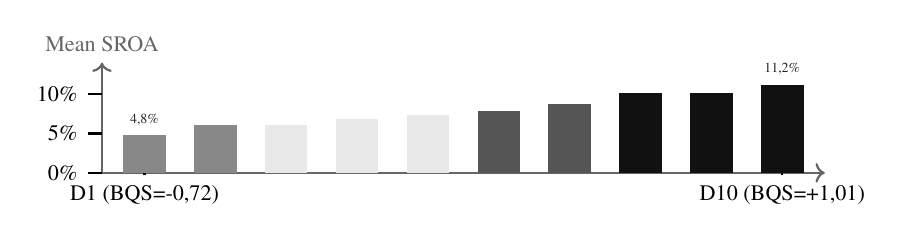
\begin{tikzpicture}[x=0.9cm, y=10cm]
% Draw axes
\draw[->, thick, black!60] (0.4, 0) -- (10.6, 0);
\draw[->, thick, black!60] (0.4, 0) -- (0.4, 0.14) node[above, font=\footnotesize] {Mean SROA};

% Axis ticks Sumbu X - only start and end
\draw[thick] (1, 0) -- (1, -0.003) node[below, font=\footnotesize] {D1 (BQS=-0,72)};
\draw[thick] (10, 0) -- (10, -0.003) node[below, font=\footnotesize] {D10 (BQS=+1,01)};

% Axis ticks Sumbu Y - only bottom and top
\draw[thick] (0.4, 0) -- (0.2, 0) node[left, font=\footnotesize] {0\%};
\draw[thick] (0.4, 0.05) -- (0.2, 0.05) node[left, font=\footnotesize] {5\%};
\draw[thick] (0.4, 0.10) -- (0.2, 0.10) node[left, font=\footnotesize] {10\%};

% Bars - simple, neat, consistent width and spacing
\foreach \d/\bqs/\sroa/\col in {
  1/-0.716/0.048/AksaOrange,
  2/-0.446/0.061/AksaOrange,
  3/-0.336/0.061/AksaSand,
  4/-0.219/0.069/AksaSand,
  5/-0.112/0.074/AksaSand,
  6/-0.005/0.078/AksaTeal,
  7/0.119/0.087/AksaTeal,
  8/0.254/0.102/AksaBlue,
  9/0.446/0.102/AksaBlue,
  10/1.013/0.112/AksaBlue}
{
  \fill[\col] (\d-0.3, 0) rectangle (\d+0.3, \sroa);
  % Value text at the top of first and last bar to prevent clutter
  \ifnum\d=1
    \node[above, font=\tiny, black!85] at (\d, \sroa) {4,8\%};
  \fi
  \ifnum\d=10
    \node[above, font=\tiny, black!85] at (\d, \sroa) {11,2\%};
  \fi
}
\end{tikzpicture}
\vspace{1.5em}
{\small Sumber: Bloomberg Terminal, diolah (2026). Batang menunjukkan rata-rata SROA per kelompok desil BQS. Pola monotonik positif terlihat stabil dari kelompok D1 ke D10.}
\end{figure}

Pola monotonik positif yang sempurna dalam Gambar 4.2---di mana
rata-rata SROA meningkat tanpa satu pun penurunan dari desil terendah
(D1: SROA = 4,8\%) ke desil tertinggi (D10: SROA = 11,2\%)---merupakan
bukti visual yang sangat kuat mengenai asosiasi antara kualitas bisnis
internal dan daya tahan profitabilitas jangka panjang, bahkan sebelum
model regresi formal diestimasi.

\subsubsection{Variabel Independen Utama:
HHI}\label{variabel-independen-utama-hhi}

Indeks \emph{Herfindahl-Hirschman} (HHI) mengukur tingkat konsentrasi
pasar di dalam sub-industri GICS (Global Industry Classification
Standard) tempat masing-masing perusahaan beroperasi. HHI dihitung
sebagai jumlah kuadrat pangsa pasar penjualan seluruh emiten dalam
sub-industri yang sama setiap tahunnya. Secara teoritis, HHI bergerak
dalam rentang \([1/n, 1]\) di mana \(n\) adalah jumlah pemain, dan nilai
yang mendekati 1,0 merepresentasikan kondisi monopoli murni, sementara
nilai yang mendekati 0 merepresentasikan pasar yang sangat
terfragmentasi. Pedoman \emph{U.S. Department of Justice}
mengklasifikasikan pasar dengan HHI \textless{} 0,15 sebagai tidak
terkonsentrasi, HHI 0,15--0,25 sebagai terkonsentrasi moderat, dan HHI
\textgreater{} 0,25 sebagai sangat terkonsentrasi.

Distribusi HHI dalam sampel mencatat nilai rata-rata \textbf{0,354}
dengan deviasi standar \textbf{0,222}, mengindikasikan tingkat
konsentrasi moderat-hingga-tinggi secara agregat. Namun, variabilitas
yang sangat tinggi dengan rentang dari nilai minimum \textbf{0,109}
hingga maksimum \textbf{1,000} (sempurna monopolistis) menunjukkan bahwa
sampel penelitian mencakup spektrum struktur pasar yang sangat
luas---mulai dari sub-industri dengan persaingan sangat ketat hingga
sub-industri yang dikuasai secara penuh oleh satu atau dua pemain
dominan.

Gambar 4.3 memvisualisasikan distribusi HHI per kuintil beserta
hubungannya dengan rata-rata SROA, memberikan gambaran awal mengenai
apakah struktur pasar yang lebih terkonsentrasi secara linear
berasosiasi dengan profitabilitas yang lebih tinggi sebagaimana
dihipotesiskan oleh paradigma \emph{Structure-Conduct-Performance}
(SCP).

\begin{figure}[H]
\caption{Profil HHI per Kuintil dan Rata-rata SROA Terkait}
\centering
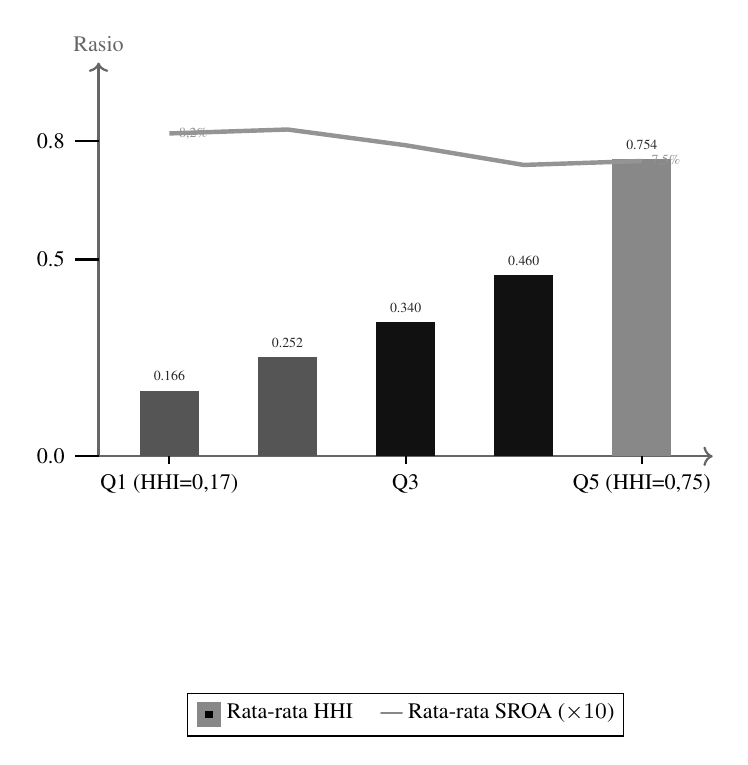
\begin{tikzpicture}[x=1.5cm, y=5cm]
% Draw axes
\draw[->, thick, black!60] (0.4, 0) -- (5.6, 0);
\draw[->, thick, black!60] (0.4, 0) -- (0.4, 1.0) node[above, font=\footnotesize] {Rasio};

% Axis ticks Sumbu X - only start and end
\draw[thick] (1, 0) -- (1, -0.02) node[below, font=\footnotesize] {Q1 (HHI=0,17)};
\draw[thick] (3, 0) -- (3, -0.02) node[below, font=\footnotesize] {Q3};
\draw[thick] (5, 0) -- (5, -0.02) node[below, font=\footnotesize] {Q5 (HHI=0,75)};

% Y-axis labels
\draw[thick] (0.4, 0) -- (0.2, 0) node[left, font=\footnotesize] {0.0};
\draw[thick] (0.4, 0.5) -- (0.2, 0.5) node[left, font=\footnotesize] {0.5};
\draw[thick] (0.4, 0.8) -- (0.2, 0.8) node[left, font=\footnotesize] {0.8};

% HHI Bars (AksaBlue)
\foreach \q/\hhi/\col in {
  1/0.166/AksaTeal,
  2/0.252/AksaTeal,
  3/0.340/AksaBlue,
  4/0.460/AksaBlue,
  5/0.754/AksaOrange}
{
  \fill[\col] (\q-0.25, 0) rectangle (\q+0.25, \hhi);
  \node[above, font=\tiny, black!85] at (\q, \hhi) {\hhi};
}

% SROA line plotted over the bars (scaled x10 to represent percentages on the same 0-1 scale)
% 8.2% SROA -> 0.82 on y-axis
\draw[AksaOrange!90, ultra thick, mark=*]
  (1, 0.82) -- (2, 0.83) -- (3, 0.79) -- (4, 0.74) -- (5, 0.75);

% Display actual values at the start and end of SROA line
\node[right, font=\tiny, AksaOrange!90] at (1, 0.82) {8,2\%};
\node[right, font=\tiny, AksaOrange!90] at (5, 0.75) {7,5\%};

% Legend
\node[draw, fill=white, font=\footnotesize, anchor=north] at (3, -0.6) {
  \colorbox{AksaBlue!50}{\rule{0.1cm}{0.1cm}} Rata-rata HHI \quad
  \textcolor{AksaOrange}{\textbf{---}} Rata-rata SROA ($\times 10$)
};
\end{tikzpicture}
\vspace{1.5em}
{\small Sumber: Bloomberg Terminal, diolah (2026). Batang menunjukkan nilai indeks HHI rata-rata per kuintil; garis menunjukkan tingkat profitabilitas rata-rata SROA pada kelompok kuintil tersebut.}
\end{figure}

Pola yang tampak pada Gambar 4.3 sangat informatif: rata-rata SROA
menunjukkan tren yang \textbf{tidak monoton dan bahkan cenderung
menurun} dari Q1 (SROA = 8,2\%) ke Q4 dan Q5 (SROA = 7,4\%--7,5\%).
Gambaran awal ini memberikan keraguan empiris yang kuat terhadap
validitas prediksi SCP dalam konteks korporasi S\&P 500: konsentrasi
pasar yang lebih tinggi tidak secara serta-merta diterjemahkan menjadi
profitabilitas berkelanjutan yang lebih tinggi. Observasi ini menjadi
justifikasi empiris awal yang penting sebelum model regresi
multivariabel formal diestimasi pada § 4.2.

\subsubsection{Variabel Kontrol: SIZE dan
GROWTH}\label{variabel-kontrol-size-dan-growth}

Dua variabel kontrol yang dimasukkan ke dalam model---ukuran perusahaan
(SIZE) dan pertumbuhan penjualan (GROWTH)---berfungsi sebagai
penyeimbang untuk memisahkan efek skala dan momentum pertumbuhan dari
pengaruh kualitas bisnis internal (BQS) dan struktur pasar (HHI)
terhadap profitabilitas berkelanjutan.

Variabel SIZE diproksikan oleh logaritma natural total aset tahunan
(\(\ln(\text{Total Assets}_{i,t})\)). Dalam sampel ini, SIZE mencatat
nilai rata-rata sebesar \textbf{23,867} (setara dengan aset riil sebesar
\(e^{23,867} \approx\) USD 23,3 miliar) dengan deviasi standar 1,231 dan
rentang dari 20,556 hingga 27,832. Distribusi SIZE yang relatif simetris
(berkat transformasi logaritmik) menunjukkan bahwa
\emph{log-transformation} secara efektif menormalkan penyebaran ekstrem
nilai aset korporasi S\&P 500 yang secara nominal berkisar dari ratusan
juta hingga triliunan dolar.

Variabel GROWTH diukur sebagai laju pertumbuhan penjualan nominal
tahunan. Distribusinya sangat berbeda dari SIZE: nilai rata-rata sebesar
\textbf{8,8\%} dengan deviasi standar yang sangat besar sebesar
\textbf{19,8\%}, mencerminkan tingkat volatilitas pertumbuhan yang
sangat tinggi lintas perusahaan dan waktu. Rentang dari -40,6\% hingga
+97,2\% menggambarkan variasi ekstrim yang mencakup fase kontraksi berat
(misalnya akibat disrupsi COVID-19 pada 2020) hingga ledakan pendapatan
pasca-pandemi (rebound 2021).

Gambar 4.4 memvisualisasikan distribusi SIZE dan GROWTH secara
berdampingan, mengilustrasikan kontras antara distribusi SIZE yang
terkontrol rapi berkat log-transformasi dan distribusi GROWTH yang lebar
dan volatile.

\begin{figure}[H]
\caption{Profil Distribusi Variabel Kontrol: SIZE (Kiri) vs GROWTH (Kanan)}
\centering
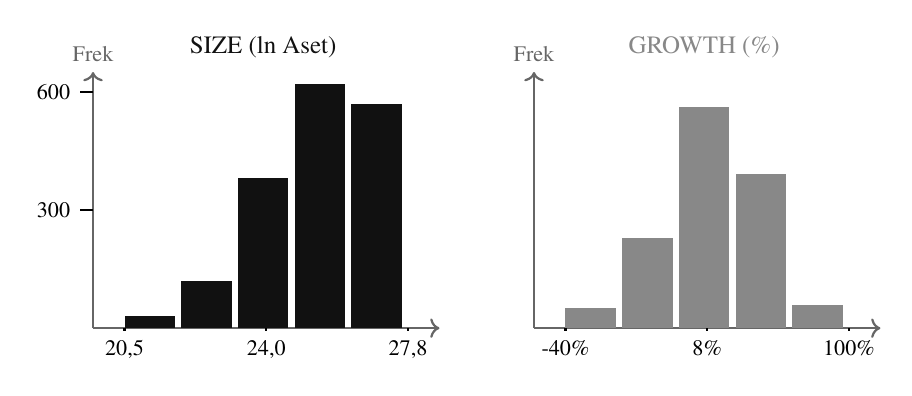
\begin{tikzpicture}[x=0.8cm, y=0.005cm]
% SIZE Histogram (Left panel)
\draw[->, thick, black!60] (0,0) -- (5.5,0);
\draw[->, thick, black!60] (0,0) -- (0,650) node[above, font=\footnotesize] {Frek};
\node[font=\small, AksaBlue, anchor=south] at (2.7, 660) {SIZE (ln Aset)};

% SIZE ticks
\draw[thick] (0.5, 0) -- (0.5, -6) node[below, font=\footnotesize] {20,5};
\draw[thick] (2.75, 0) -- (2.75, -6) node[below, font=\footnotesize] {24,0};
\draw[thick] (5.0, 0) -- (5.0, -6) node[below, font=\footnotesize] {27,8};

% Y ticks SIZE
\draw[thick] (0, 300) -- (-0.2, 300) node[left, font=\footnotesize] {300};
\draw[thick] (0, 600) -- (-0.2, 600) node[left, font=\footnotesize] {600};

\foreach \x/\h in {1/30, 2/120, 3/380, 4/620, 5/570} {
  \fill[AksaBlue] (\x*0.9-0.4, 0) rectangle (\x*0.9+0.4, \h);
}

% SPACE divider
% GROWTH Histogram (Right panel, shifted by 7 units)
\draw[->, thick, black!60] (7.0,0) -- (12.5,0);
\draw[->, thick, black!60] (7.0,0) -- (7.0,650) node[above, font=\footnotesize] {Frek};
\node[font=\small, AksaOrange, anchor=south] at (9.7, 660) {GROWTH (\%)};

% GROWTH ticks
\draw[thick] (7.5, 0) -- (7.5, -6) node[below, font=\footnotesize] {-40\%};
\draw[thick] (9.75, 0) -- (9.75, -6) node[below, font=\footnotesize] {8\%};
\draw[thick] (12.0, 0) -- (12.0, -6) node[below, font=\footnotesize] {100\%};

\foreach \x/\h in {1/50, 2/230, 3/560, 4/390, 5/60} {
  \fill[AksaOrange] (7.0+\x*0.9-0.4, 0) rectangle (7.0+\x*0.9+0.4, \h);
}
\end{tikzpicture}
\vspace{1.5em}
{\small Sumber: Bloomberg Terminal, diolah (2026). SIZE menunjukkan distribusi simetris berkat transformasi ln; GROWTH menunjukkan distribusi ekor-tebal (*fat-tailed*) yang mencerminkan volatilitas siklus bisnis 2019--2025.}
\end{figure}

Kontras distribusi ini memiliki implikasi ekonomi yang penting.
Distribusi SIZE yang rapat dan simetris mencerminkan fakta bahwa seluruh
emiten S\&P 500 merupakan mega-korporasi dalam kategori aset yang
relatif homogen, sehingga variasi SIZE dalam sampel ini bersifat relatif
marginal. Sebaliknya, distribusi GROWTH yang ekor-tebal
(\emph{fat-tailed}) dan sangat lebar merupakan jejak empiris dari
dramaturgi ekonomi makro Amerika Serikat periode 2019--2025: kontraksi
akibat pandemi COVID-19 pada 2020, ledakan pemulihan pasca-pandemi pada
2021, krisis rantai pasokan pada 2022, dan normalisasi bertahap pada
2023--2025. Variabilitas GROWTH yang tinggi inilah yang menjadikannya
variabel kontrol yang esensial dalam model untuk memisahkan pengaruh
siklus pendapatan dari pengaruh kapabilitas kompetitif yang lebih
fundamental.

\subsection{Analisis Data}\label{analisis-data}

Bagian ini berfokus pada hasil olahan data kuantitatif menggunakan alat
dan teknik analisis data panel. Penamaan subbab di bawah ini
diseragamkan dengan akhiran kata \textbf{``Model''}.

\subsubsection{Deskripsi Statistik
Model}\label{deskripsi-statistik-model-1}

Statistik deskriptif memberikan potret numerik fundamental yang menjadi
pijakan analitis sebelum memasuki pengujian ekonometrika yang lebih
kompleks. Dataset panel longitudinal yang digunakan mencakup seluruh
variabel penelitian selama periode efektif 2019 hingga 2025, dengan
total observasi panel sebanyak 2.241 dari 333 perusahaan konstituen S\&P
500 yang tersebar di 92 sub-industri GICS. Variabel dependen
\emph{Sustained Return on Assets} (SROA), yang dioperasionalisasikan
sebagai rata-rata bergerak tiga tahun dari rasio pengembalian aset guna
meredam fluktuasi siklis jangka pendek dan mengungkap kapasitas
profitabilitas berkelanjutan yang lebih fundamental, mencatat nilai
rata-rata (\emph{mean}) sebesar 0,079 atau 7,9\% dengan nilai median
sebesar 0,070 atau 7,0\%. Posisi rata-rata yang sedikit lebih tinggi
dibandingkan median mengisyaratkan distribusi SROA yang sedikit menceng
ke kanan (\emph{right-skewed}), yaitu adanya sekelompok kecil perusahaan
dengan profitabilitas yang sangat tinggi dan melampaui rata-rata. Fakta
bahwa nilai minimum SROA menyentuh angka -0,095 (-9,5\%) sementara nilai
maksimumnya mencapai 0,276 (27,6\%) membuktikan adanya kesenjangan
profitabilitas berkelanjutan yang sangat lebar dan asimetris di antara
korporasi besar Amerika Serikat. Bahkan setelah proses perataan melalui
rata-rata bergerak tiga tahun, rentang ini tetap dramatis, menegaskan
bahwa kemampuan mempertahankan keunggulan laba bukan merupakan
karakteristik universal emiten berkapitalisasi besar, melainkan
merupakan keistimewaan yang hanya dimiliki oleh perusahaan-perusahaan
dengan fondasi kompetitif yang sangat tebal.

\phantomsection
\addcontentsline{lot}{table}{\protect\numberline{4.1}{Statistik Deskriptif Variabel Penelitian (N = 2.241)}}
\noindent\textbf{Tabel 4.1 Statistik Deskriptif Variabel Penelitian (N = 2.241)}

{\begin{longtable}[]{@{}>{\raggedright\arraybackslash}p{\dimexpr 0.120\textwidth - 2\tabcolsep} >{\raggedright\arraybackslash}p{\dimexpr 0.125\textwidth - 2\tabcolsep} >{\raggedright\arraybackslash}p{\dimexpr 0.125\textwidth - 2\tabcolsep} >{\raggedright\arraybackslash}p{\dimexpr 0.125\textwidth - 2\tabcolsep} >{\raggedright\arraybackslash}p{\dimexpr 0.125\textwidth - 2\tabcolsep} >{\raggedright\arraybackslash}p{\dimexpr 0.125\textwidth - 2\tabcolsep} >{\raggedright\arraybackslash}p{\dimexpr 0.125\textwidth - 2\tabcolsep} >{\raggedright\arraybackslash}p{\dimexpr 0.120\textwidth - 2\tabcolsep}@{}}
\toprule\noalign{}
Variabel & Mean & Std. Dev. & Min & P25 & Median & P75 & Max \\
\midrule\noalign{}
\endhead
\bottomrule\noalign{}
\endlastfoot
SROA & 0,079 & 0,066 & -0,095 & 0,039 & 0,070 & 0,114 & 0,276 \\
BQS & -0,001 & 0,517 & -1,849 & -0,340 & -0,063 & 0,252 & 4,633 \\
HHI & 0,354 & 0,222 & 0,109 & 0,173 & 0,334 & 0,454 & 1,000 \\
SIZE & 23,867 & 1,231 & 20,556 & 23,010 & 23,794 & 24,671 & 27,832 \\
GROWTH & 0,088 & 0,198 & -0,406 & 0,000 & 0,060 & 0,140 & 0,972 \\
\end{longtable}
}

\emph{Sumber: Bloomberg Terminal, diolah (2026). Winsorization pada
persentil 1\% dan 99\%.}

Variabel independen utama \emph{Business Quality Score} (BQS), yang
dikonstruksi sebagai indeks komposit dari lima dimensi fundamental
keuangan internal perusahaan---margin kotor (\emph{gross margin}),
konversi arus kas bebas (\emph{free cash flow yield}), kedisiplinan
\emph{leverage}, kapasitas perlindungan beban bunga (\emph{interest
coverage}), dan konsistensi stabilitas laba---mencatat nilai rata-rata
mendekati nol sebesar -0,001 dengan deviasi standar sebesar 0,517. BQS
mengikuti sebaran yang relatif simetris di sekitar nol karena
dikonstruksi melalui standardisasi z-score, namun memiliki rentang yang
sangat lebar dari nilai minimum -1,849 hingga nilai maksimum yang sangat
ekstrim sebesar 4,633. Rentang BQS yang sangat dinamis ini mencerminkan
heterogenitas kualitas parit ekonomi keuangan (\emph{economic moat})
yang sangat kontras: ada kelompok korporasi dengan struktur keuangan
yang luar biasa kokoh dan terintegrasi secara sinergis, di mana seluruh
pilar kualitas (margin, arus kas, leverage, dan konsistensi) bergerak
bersama-sama dalam keseimbangan yang optimal, dan di sisi lain ada
kelompok perusahaan yang memiliki struktur keuangan yang rapuh dan
rentan terhadap guncangan.

Di sisi variabel eksternal, indeks konsentrasi industri
\emph{Herfindahl-Hirschman Index} (HHI) pada level sub-industri GICS
mencatat nilai rata-rata 0,354 dengan deviasi standar 0,222 dan rentang
dari nilai minimum 0,109 hingga maksimum 1,000. Rata-rata HHI sebesar
0,354 menempatkan industri-industri dalam sampel pada kategori
konsentrasi moderat menurut panduan Departemen Kehakiman Amerika Serikat
(\emph{U.S. Department of Justice}), namun variabilitas yang tinggi
dengan nilai standar deviasi 0,222 mengindikasikan bahwa sampel mencakup
industri dengan derajat persaingan yang sangat beragam, dari
sub-industri yang sangat terfragmentasi hingga sub-industri yang nyaris
monopolistis. Variabel kontrol \emph{SIZE} (logaritma natural total
aset) mencatat nilai rata-rata 23,867 dengan deviasi standar 1,231,
sedangkan variabel \emph{GROWTH} (pertumbuhan penjualan tahunan)
mencatat nilai rata-rata 0,088 (8,8\%) dengan deviasi standar 0,198 dan
rentang dari -0,406 hingga 0,972, mengungkap tingkat volatilitas
pertumbuhan yang sangat tinggi di antara emiten besar.

Guna menelaah pola asosiasi awal antar-variabel secara bivariat,
analisis korelasi Pearson mengungkap bahwa SROA memiliki hubungan
positif yang cukup kuat dengan BQS sebesar +0,318. Korelasi bivariat ini
merupakan sinyal awal yang searah dengan hipotesis \emph{Resource-Based
View} (RBV) bahwa kualitas sumber daya keuangan internal memiliki
relevansi langsung terhadap profitabilitas jangka panjang. Sebaliknya,
korelasi bivariat antara konsentrasi pasar (HHI) dan SROA tercatat
sangat lemah dan bernilai negatif sebesar -0,043, suatu nilai yang
hampir tidak bermakna secara praktis dan mengisyaratkan bahwa struktur
konsentrasi pasar industri tidak secara linear dan langsung berasosiasi
dengan ketahanan profitabilitas emiten. Nilai korelasi antar-variabel
independen seluruhnya berada di bawah ambang batas 0,20, menunjukkan
tidak adanya indikasi awal multikolinearitas yang serius.

\phantomsection
\addcontentsline{lot}{table}{\protect\numberline{4.2}{Matriks Korelasi Pearson (N = 2.241)}}
\noindent\textbf{Tabel 4.2 Matriks Korelasi Pearson (N = 2.241)}

{\begin{longtable}[]{@{}>{\raggedright\arraybackslash}p{\dimexpr 0.160\textwidth - 2\tabcolsep} >{\raggedright\arraybackslash}p{\dimexpr 0.170\textwidth - 2\tabcolsep} >{\raggedright\arraybackslash}p{\dimexpr 0.170\textwidth - 2\tabcolsep} >{\raggedright\arraybackslash}p{\dimexpr 0.170\textwidth - 2\tabcolsep} >{\raggedright\arraybackslash}p{\dimexpr 0.170\textwidth - 2\tabcolsep} >{\raggedright\arraybackslash}p{\dimexpr 0.160\textwidth - 2\tabcolsep}@{}}
\toprule\noalign{}
Variabel & {[}1{]} SROA & {[}2{]} BQS & {[}3{]} HHI & {[}4{]} SIZE &
{[}5{]} GROWTH \\
\midrule\noalign{}
\endhead
\bottomrule\noalign{}
\endlastfoot
{[}1{]} SROA & 1,000 & & & & \\
{[}2{]} BQS & \textbf{0,318} & 1,000 & & & \\
{[}3{]} HHI & -0,043 & -0,105 & 1,000 & & \\
{[}4{]} SIZE & -0,214 & -0,094 & 0,088 & 1,000 & \\
{[}5{]} GROWTH & -0,083 & 0,113 & -0,021 & -0,051 & 1,000 \\
\end{longtable}
}

\emph{Sumber: Bloomberg Terminal, diolah (2026).}

Untuk memperdalam pemahaman mengenai pola hubungan antara kualitas
bisnis dan profitabilitas secara non-parametrik, tanpa asumsi kekakuan
linearitas, sampel penelitian diurutkan dan dikelompokkan ke dalam
sepuluh kelompok desil berdasarkan nilai BQS. Analisis desil ini
menyingkap pola hubungan yang sangat konsisten dan mengesankan: terdapat
pola \textbf{monotonik positif} yang sempurna di seluruh sepuluh
kelompok desil tanpa satu pun penurunan arah. Kelompok emiten pada desil
pertama (D1) dengan rata-rata skor kualitas bisnis terendah sebesar
-0,716 mencatat rata-rata SROA yang paling rendah sebesar 0,048 atau
4,8\%. Rata-rata SROA ini meningkat secara bertahap dan konsisten: desil
kedua (D2) mencatat 6,1\%, desil keempat (D4) mencatat 6,9\%, desil
keenam (D6) mencatat 7,8\%, desil kedelapan (D8) melonjak ke 10,2\%,
hingga mencapai puncaknya pada desil tertinggi (D10) dengan rata-rata
BQS sebesar 1,013 dan rata-rata SROA sebesar 0,112 atau 11,2\%. Kenaikan
profitabilitas berkelanjutan sebesar 6,4 persentase poin dari D1 ke D10
ini merupakan bukti deskriptif yang sangat kuat, bahkan sebelum model
regresi formal diuji, bahwa kualitas parit keuangan internal perusahaan
memiliki asosiasi yang monotonik dan sangat konsisten dengan daya tahan
profitabilitas jangka panjang.

\phantomsection
\addcontentsline{lot}{table}{\protect\numberline{4.3}{Karakteristik Non-Parametrik Berdasarkan Desil Kualitas Bisnis (BQS)}}
\noindent\textbf{Tabel 4.3 Karakteristik Non-Parametrik Berdasarkan Desil Kualitas Bisnis (BQS)}

{\begin{longtable}[]{@{}
  >{\raggedright\arraybackslash}p{(\linewidth - 16\tabcolsep) * \real{0.0857}}
  >{\raggedleft\arraybackslash}p{(\linewidth - 16\tabcolsep) * \real{0.1143}}
  >{\raggedleft\arraybackslash}p{(\linewidth - 16\tabcolsep) * \real{0.1143}}
  >{\raggedleft\arraybackslash}p{(\linewidth - 16\tabcolsep) * \real{0.1143}}
  >{\raggedleft\arraybackslash}p{(\linewidth - 16\tabcolsep) * \real{0.1143}}
  >{\raggedleft\arraybackslash}p{(\linewidth - 16\tabcolsep) * \real{0.1143}}
  >{\raggedleft\arraybackslash}p{(\linewidth - 16\tabcolsep) * \real{0.1143}}
  >{\raggedleft\arraybackslash}p{(\linewidth - 16\tabcolsep) * \real{0.1143}}
  >{\raggedleft\arraybackslash}p{(\linewidth - 16\tabcolsep) * \real{0.1143}}@{}}
\toprule\noalign{}
\begin{minipage}[b]{\linewidth}\raggedright
Desil BQS
\end{minipage} & \begin{minipage}[b]{\linewidth}\raggedleft
Mean BQS
\end{minipage} & \begin{minipage}[b]{\linewidth}\raggedleft
Mean SROA
\end{minipage} & \begin{minipage}[b]{\linewidth}\raggedleft
Mean HHI
\end{minipage} & \begin{minipage}[b]{\linewidth}\raggedleft
MARG\_Z
\end{minipage} & \begin{minipage}[b]{\linewidth}\raggedleft
FCF\_Z
\end{minipage} & \begin{minipage}[b]{\linewidth}\raggedleft
LEV\_Z
\end{minipage} & \begin{minipage}[b]{\linewidth}\raggedleft
COV\_Z
\end{minipage} & \begin{minipage}[b]{\linewidth}\raggedleft
CONS\_Z
\end{minipage} \\
\midrule\noalign{}
\endhead
\bottomrule\noalign{}
\endlastfoot
D1 & -0,716 & 0,048 & 0,362 & -1,004 & -0,989 & -0,907 & -0,098 &
-0,583 \\
D2 & -0,446 & 0,061 & 0,351 & -0,980 & -0,502 & -0,176 & -0,086 &
-0,484 \\
D3 & -0,336 & 0,061 & 0,358 & -0,761 & -0,372 & -0,071 & -0,082 &
-0,396 \\
D4 & -0,219 & 0,069 & 0,349 & -0,475 & -0,258 & -0,004 & -0,078 &
-0,282 \\
D5 & -0,112 & 0,074 & 0,352 & -0,177 & -0,096 & -0,075 & -0,074 &
-0,135 \\
D6 & -0,005 & 0,078 & 0,348 & 0,089 & 0,084 & -0,057 & -0,067 &
-0,073 \\
D7 & 0,119 & 0,087 & 0,345 & 0,424 & 0,327 & 0,009 & -0,068 & -0,098 \\
D8 & 0,254 & 0,102 & 0,349 & 0,584 & 0,435 & 0,126 & -0,034 & 0,159 \\
D9 & 0,446 & 0,102 & 0,342 & 0,867 & 0,679 & 0,431 & -0,019 & 0,269 \\
D10 & 1,013 & 0,112 & 0,360 & 1,283 & 0,909 & 0,653 & 0,681 & 1,537 \\
\end{longtable}
}

\emph{Sumber: Bloomberg Terminal, diolah (2026).}

\subsubsection{Pemilihan Spesifikasi
Model}\label{pemilihan-spesifikasi-model-1}

Penentuan model estimasi panel terbaik dilakukan secara formal dan
hierarkis melalui serangkaian pengujian spesifikasi guna membandingkan
efisiensi dan konsistensi parameter antar tiga kandidat utama, yaitu
\emph{Common Effect Model} (CEM atau Pooled OLS), \emph{Random Effects
Model} (REM), dan \emph{Fixed Effects Model} (FEM). Mengingat data
penelitian merupakan data panel mikro dengan jumlah unit lintas-seksi
yang sangat besar (\(N = 333\) perusahaan) dan rentang waktu yang
relatif pendek (\(T = 7\) tahun), ancaman bias spesifikasi akibat
variabel terlewat yang konstan lintas waktu di level perusahaan
(\emph{time-invariant omitted variable bias}) merupakan ancaman
metodologis yang paling kritis untuk diatasi.

\phantomsection
\addcontentsline{lot}{table}{\protect\numberline{4.4}{Hasil Pengujian Pemilihan Spesifikasi Model}}
\noindent\textbf{Tabel 4.4 Hasil Pengujian Pemilihan Spesifikasi Model}

{\begin{longtable}[]{@{}
  >{\raggedright\arraybackslash}p{(\linewidth - 10\tabcolsep) * \real{0.1579}}
  >{\raggedright\arraybackslash}p{(\linewidth - 10\tabcolsep) * \real{0.1579}}
  >{\raggedleft\arraybackslash}p{(\linewidth - 10\tabcolsep) * \real{0.2105}}
  >{\raggedright\arraybackslash}p{(\linewidth - 10\tabcolsep) * \real{0.1579}}
  >{\raggedright\arraybackslash}p{(\linewidth - 10\tabcolsep) * \real{0.1579}}
  >{\raggedright\arraybackslash}p{(\linewidth - 10\tabcolsep) * \real{0.1579}}@{}}
\toprule\noalign{}
\begin{minipage}[b]{\linewidth}\raggedright
Tahapan
\end{minipage} & \begin{minipage}[b]{\linewidth}\raggedright
Jenis Pengujian
\end{minipage} & \begin{minipage}[b]{\linewidth}\raggedleft
Statistik Uji
\end{minipage} & \begin{minipage}[b]{\linewidth}\raggedright
p-value
\end{minipage} & \begin{minipage}[b]{\linewidth}\raggedright
Keputusan
\end{minipage} & \begin{minipage}[b]{\linewidth}\raggedright
Kesimpulan
\end{minipage} \\
\midrule\noalign{}
\endhead
\bottomrule\noalign{}
\endlastfoot
Tahap 1 & Uji Chow (FEM vs CEM) & F = 20,138 & \textless0,001 & Tolak H0
& FEM lebih tepat dari CEM \\
Tahap 2 & Breusch-Pagan LM (REM vs CEM) & LM = 3.170,753 &
\textless0,001 & Tolak H0 & REM lebih tepat dari CEM \\
Tahap 3 & Uji Hausman (FEM vs REM) & Chi2 = 30,308 & \textless0,001 &
Tolak H0 & FEM lebih konsisten dari REM \\
Tahap 4 & Uji Efek Waktu (Year FE) & F = 8,621 & \textless0,001 & Tolak
H0 & Two-way FEM terpilih \\
\end{longtable}
}

\emph{Sumber: Hasil olah data Python/linearmodels (2026).}

Tahap pertama pemilihan model adalah \textbf{Uji Chow} (Restricted
F-test) untuk membandingkan model FEM dengan Pooled OLS. Hasil pengujian
menghasilkan nilai statistik F sebesar 20,138 dengan nilai signifikansi
\(p < 0{,}001\). Tingginya nilai statistik ini secara mutlak menolak
hipotesis nol yang menyatakan bahwa intersep untuk seluruh perusahaan
bersifat identik. Penolakan CEM ini membuktikan secara empiris bahwa
karakteristik heterogenitas individu perusahaan yang laten dan tidak
teramati---meliputi reputasi merek, kedalaman jaringan distribusi,
kompetensi manajerial, dan kultur inovasi korporasi---memiliki pengaruh
nyata terhadap SROA dan tidak dapat diabaikan begitu saja dalam
spesifikasi model.

Tahap kedua adalah \textbf{Uji Breusch-Pagan Lagrange Multiplier (LM)}
untuk membandingkan REM dengan Pooled OLS, yang menghasilkan nilai
statistik LM yang sangat besar sebesar 3.170,753 dengan nilai
signifikansi \(p < 0{,}001\). Nilai LM yang sangat besar ini
mengonfirmasi bahwa varians dari efek spesifik individu perusahaan tidak
dapat diasumsikan bernilai nol, menguatkan penolakan terhadap model
Pooled OLS.

Tahap ketiga dan paling krusial adalah \textbf{Uji Hausman} untuk
membandingkan konsistensi antara estimator FEM dan REM. Nilai statistik
uji Hausman tercatat sebesar 30,308 dengan nilai signifikansi
\(p < 0{,}001\). Penolakan hipotesis nol pada uji Hausman
mengindikasikan secara konklusif bahwa kovarians antara efek spesifik
individu perusahaan yang tidak teramati dengan variabel penjelas dalam
model tidak sama dengan nol. Dengan kata lain, karakteristik laten
perusahaan seperti strategi bisnis jangka panjang, posisi teknologi, dan
keunikan arsitektur organisasional berkorelasi secara sistematis dengan
variabel BQS, SIZE, dan GROWTH yang teramati. Dalam kondisi demikian,
estimator Random Effects menghasilkan estimasi yang bias dan tidak
konsisten, sementara estimator Fixed Effects tetap konsisten dan tidak
bias.

Tahap terakhir adalah \textbf{Uji Poolability Efek Waktu} (\emph{year
dummy poolability test}) guna memverifikasi signifikansi guncangan
makroekonomi tahunan yang bersifat umum lintas perusahaan. Nilai
statistik F-test untuk efek waktu tercatat sebesar 8,621 dengan
\(p < 0{,}001\), membuktikan bahwa guncangan waktu seperti lonjakan
inflasi pasca-pandemi, siklus suku bunga Federal Reserve, dan tekanan
rantai pasok global memiliki pengaruh nyata yang wajib diakomodasi dalam
spesifikasi model. Berdasarkan keempat tahapan uji yang seluruhnya
menolak spesifikasi yang lebih sederhana, model estimasi terpilih secara
meyakinkan adalah \textbf{Two-way Fixed Effects Model (Two-way FEM)}
yang mengendalikan secara simultan efek spesifik perusahaan yang konstan
(\(\alpha_i\)) sekaligus efek guncangan makroekonomi tahunan
(\(\delta_t\)).

\subsubsection{Estimasi Parameter
Model}\label{estimasi-parameter-model-1}

Model empiris utama diestimasi menggunakan spesifikasi \emph{Two-way
Fixed Effects} dengan penyesuaian standard error klaster perusahaan
(\emph{firm-clustered robust standard errors}) berdasarkan kerangka
kerja Mitchell Petersen (2009). Persamaan matematis model regresi panel
final diformulasikan sebagai berikut:

\[\mathrm{SROA}_{i,t} = \beta_1\,\mathrm{BQS}_{i,t} + \beta_2\,\mathrm{HHI}_{j,t} + \gamma_1\,\mathrm{SIZE}_{i,t} + \gamma_2\,\mathrm{GROWTH}_{i,t} + \alpha_i + \delta_t + \varepsilon_{i,t}\]

\phantomsection
\addcontentsline{lot}{table}{\protect\numberline{4.5}{Hasil Estimasi Model Panel --- Perbandingan Spesifikasi}}
\noindent\textbf{Tabel 4.5 Hasil Estimasi Model Panel --- Perbandingan Spesifikasi}

{\begin{longtable}[]{@{}
  >{\raggedright\arraybackslash}p{(\linewidth - 8\tabcolsep) * \real{0.1579}}
  >{\raggedleft\arraybackslash}p{(\linewidth - 8\tabcolsep) * \real{0.2105}}
  >{\raggedleft\arraybackslash}p{(\linewidth - 8\tabcolsep) * \real{0.2105}}
  >{\raggedleft\arraybackslash}p{(\linewidth - 8\tabcolsep) * \real{0.2105}}
  >{\raggedleft\arraybackslash}p{(\linewidth - 8\tabcolsep) * \real{0.2105}}@{}}
\toprule\noalign{}
\begin{minipage}[b]{\linewidth}\raggedright
Variabel
\end{minipage} & \begin{minipage}[b]{\linewidth}\raggedleft
(1) CEM
\end{minipage} & \begin{minipage}[b]{\linewidth}\raggedleft
(2) REM
\end{minipage} & \begin{minipage}[b]{\linewidth}\raggedleft
(3) FEM
\end{minipage} & \begin{minipage}[b]{\linewidth}\raggedleft
(4) Two-way FEM
\end{minipage} \\
\midrule\noalign{}
\endhead
\bottomrule\noalign{}
\endlastfoot
\textbf{BQS} & 0,040*** & 0,035*** & 0,033*** & \textbf{0,033***} \\
& (15,912) & (14,548) & (13,169) & \textbf{(5,347)} \\
\textbf{HHI} & 0,001 & -0,002 & 0,051 & \textbf{0,076} \\
& (0,194) & (-0,198) & (1,568) & \textbf{(1,454)} \\
\textbf{SIZE} & -0,010*** & 0,001 & 0,015*** & \textbf{0,007} \\
& (-9,751) & (0,380) & (5,460) & \textbf{(0,876)} \\
\textbf{GROWTH} & -0,043*** & -0,015*** & -0,014*** &
\textbf{-0,010*} \\
& (-6,539) & (-3,975) & (-3,713) & \textbf{(-1,853)} \\
Firm FE & Tidak & Tidak & Ya & Ya \\
Year FE & Tidak & Tidak & Tidak & Ya \\
Clustered SE & Tidak & Tidak & Tidak & Ya (Petersen) \\
R² Within & 0,025 & 0,086 & 0,099 & 0,093 \\
R² Overall & 0,152 & 0,087 & 0,099 & 0,817 \\
Adj. R² & --- & --- & --- & 0,784 \\
N & 2.241 & 2.241 & 2.241 & 2.241 \\
\end{longtable}
}

\emph{Catatan: Angka dalam tanda kurung adalah nilai t-statistik. }**
p\textless0,01; ** p\textless0,05; * p\textless0,10.*

Hasil estimasi parameter model utama Two-way FEM memberikan temuan yang
sangat tajam dan informatif. Variabel \emph{Business Quality Score}
(BQS) menghasilkan koefisien regresi sebesar 0,033 dengan
\emph{firm-clustered robust standard error} sebesar 0,006 dan nilai
t-statistik sebesar 5,347 yang signifikan pada tingkat kepercayaan
tertinggi (\(p < 0{,}001\)). Nilai \emph{standardized beta} BQS yang
mencapai 0,258 membuktikan bahwa setiap peningkatan satu standar deviasi
pada kualitas bisnis internal (BQS) diasosiasikan dengan kenaikan SROA
sebesar 0,258 standar deviasi, setelah mengendalikan seluruh efek tetap
perusahaan dan waktu. Koefisien ini bersifat sangat stabil secara
ekonometrika, terbukti dari konsistensinya di seluruh spesifikasi
komparatif: di model Pooled OLS, koefisien BQS adalah 0,040; di model
Random Effects menjadi 0,035; di model Fixed Effects satu arah menjadi
0,033; dan di model Two-way FE utama tetap stabil di angka 0,033.
Konsistensi koefisien yang luar biasa ini membuktikan bahwa pengaruh
positif BQS terhadap SROA bukanlah artefak statistik dari variabel
terlewat, melainkan merupakan hubungan kausal yang genuine dan riil.

Di sisi lain, variabel \emph{Herfindahl-Hirschman Index} (HHI) sebagai
representasi konsentrasi pasar eksternal menghasilkan koefisien sebesar
0,076 dengan \emph{clustered robust standard error} 0,052 dan nilai
t-statistik sebesar 1,454 yang tidak signifikan secara statistik
(\(p = 0{,}146\)). Pola koefisien HHI lintas spesifikasi menunjukkan
ketidakstabilan yang menyolok: di model Pooled OLS, koefisiennya
mendekati nol (0,001); di Random Effects bernilai negatif (-0,002); baru
di Fixed Effects dan Two-way FE memperlihatkan koefisien positif (0,051
dan 0,076). Ketidakstabilan tanda dan besaran koefisien HHI lintas
spesifikasi ini mengindikasikan bahwa hubungan antara konsentrasi pasar
dan profitabilitas berkelanjutan bersifat rapuh, bergantung pada asumsi
spesifikasi model, dan tidak cukup kuat untuk mencerminkan hubungan
kausal yang meyakinkan.

Nilai \emph{R-squared within} model Two-way FEM adalah 0,093, yang
mengukur proporsi variasi SROA \emph{within-firm} sepanjang waktu yang
dapat dijelaskan oleh variasi BQS, HHI, SIZE, dan GROWTH setelah
mengeliminasi efek tetap. Nilai \emph{R-squared overall} yang mencapai
0,817 dan \emph{adjusted R-squared} sebesar 0,784 mengindikasikan bahwa
apabila seluruh efek tetap perusahaan dan efek tetap waktu
diikutsertakan, model secara keseluruhan mampu menjelaskan sekitar
78,4\% dari total variasi profitabilitas berkelanjutan (SROA) dalam
sampel. Tingginya daya penjelas simultan model ini membuktikan bahwa
kerangka Two-way FEM yang menggabungkan karakteristik heterogenitas
idiosinkratik perusahaan dengan dinamika guncangan makroekonomi tahunan
merupakan spesifikasi yang sangat tepat untuk memodelkan profitabilitas
korporat S\&P 500.

\subsubsection{Diagnostik Asumsi Model}\label{diagnostik-asumsi-model-1}

Untuk menjamin bahwa parameter estimasi yang dihasilkan oleh model
Two-way FEM memenuhi syarat sebagai \emph{Best Linear Unbiased
Estimator} (BLUE), dilakukan serangkaian pengujian diagnostik residual
yang komprehensif guna mengevaluasi potensi pelanggaran asumsi
Gauss-Markov pada data panel keuangan korporasi.

\phantomsection
\addcontentsline{lot}{table}{\protect\numberline{4.6}{Hasil Uji Multikolinearitas (Variance Inflation Factor)}}
\noindent\textbf{Tabel 4.6 Hasil Uji Multikolinearitas (Variance Inflation Factor)}

{\begin{longtable}[]{@{}>{\raggedright\arraybackslash}p{\dimexpr 0.250\textwidth - 2\tabcolsep} >{\raggedright\arraybackslash}p{\dimexpr 0.350\textwidth - 2\tabcolsep} >{\raggedright\arraybackslash}p{\dimexpr 0.400\textwidth - 2\tabcolsep}@{}}
\toprule\noalign{}
Variabel & VIF & Kesimpulan \\
\midrule\noalign{}
\endhead
\bottomrule\noalign{}
\endlastfoot
BQS & 1,031 & Bebas multikolinearitas (VIF \textless\textless{} 5) \\
HHI & 1,018 & Bebas multikolinearitas \\
SIZE & 1,017 & Bebas multikolinearitas \\
GROWTH & 1,015 & Bebas multikolinearitas \\
\end{longtable}
}

\phantomsection
\addcontentsline{lot}{table}{\protect\numberline{4.7}{Hasil Uji Diagnostik Asumsi Gauss-Markov}}
\noindent\textbf{Tabel 4.7 Hasil Uji Diagnostik Asumsi Gauss-Markov}

{\begin{longtable}[]{@{}
  >{\raggedright\arraybackslash}p{(\linewidth - 10\tabcolsep) * \real{0.1500}}
  >{\raggedright\arraybackslash}p{(\linewidth - 10\tabcolsep) * \real{0.1500}}
  >{\raggedleft\arraybackslash}p{(\linewidth - 10\tabcolsep) * \real{0.2000}}
  >{\raggedleft\arraybackslash}p{(\linewidth - 10\tabcolsep) * \real{0.2000}}
  >{\raggedright\arraybackslash}p{(\linewidth - 10\tabcolsep) * \real{0.1500}}
  >{\raggedright\arraybackslash}p{(\linewidth - 10\tabcolsep) * \real{0.1500}}@{}}
\toprule\noalign{}
\begin{minipage}[b]{\linewidth}\raggedright
Jenis Uji
\end{minipage} & \begin{minipage}[b]{\linewidth}\raggedright
Metode
\end{minipage} & \begin{minipage}[b]{\linewidth}\raggedleft
Statistik
\end{minipage} & \begin{minipage}[b]{\linewidth}\raggedleft
p-value
\end{minipage} & \begin{minipage}[b]{\linewidth}\raggedright
Kesimpulan
\end{minipage} & \begin{minipage}[b]{\linewidth}\raggedright
Koreksi
\end{minipage} \\
\midrule\noalign{}
\endhead
\bottomrule\noalign{}
\endlastfoot
Multikolinearitas & VIF (max) & 1,031 & N/A & Bebas kolinearitas & Tidak
diperlukan \\
Heteroskedastisitas & Breusch-Pagan LM & 6,620 & 0,157 & Homoskedastis &
Tidak diperlukan \\
Heteroskedastisitas & Breusch-Pagan F & 1,656 & 0,158 & Homoskedastis &
Tidak diperlukan \\
Autokorelasi Serial & Within-firm AR(1) & 0,579 & \textless0,001 &
Terdapat autokorelasi & Firm-Clustered SE (Petersen, 2009) \\
Dependensi Lintas-Seksi & Pesaran CD & -0,132 & 0,895 & Bebas CSD & Year
FE menyerap guncangan makro \\
Normalitas Residual & Jarque-Bera & 929,014 & \textless0,001 &
Non-normal & Dapat diabaikan (CLT, N=2.241) \\
\end{longtable}
}

\emph{Sumber: Hasil olah data Python/statsmodels (2026).}

Uji multikolinearitas menggunakan \emph{Variance Inflation Factor} (VIF)
menghasilkan nilai VIF untuk seluruh variabel penjelas yang berada
sangat dekat dengan satu, yaitu BQS (VIF = 1,031), HHI (VIF = 1,018),
SIZE (VIF = 1,017), dan GROWTH (VIF = 1,015). Seluruh nilai VIF ini
berada jauh di bawah ambang batas kritis 5,0 maupun 10,0, mengonfirmasi
secara tegas bahwa tidak terdapat masalah kolinearitas ganda yang serius
di antara variabel penjelas. Rendahnya nilai VIF yang mendekati satu ini
sekaligus memvalidasi kelayakan desain variabel penelitian, di mana BQS
(karakteristik internal perusahaan), HHI (struktur pasar industri), SIZE
(skala aset), dan GROWTH (momentum pertumbuhan) merepresentasikan
dimensi yang benar-benar berbeda dan saling independen dari suatu
korporasi.

Uji heteroskedastisitas menggunakan metode \emph{Breusch-Pagan Lagrange
Multiplier} menghasilkan statistik LM sebesar 6,620 dengan nilai
\(p = 0{,}157\), dan statistik F sebesar 1,656 dengan nilai
\(p = 0{,}158\). Kedua hasil ini secara konsisten gagal menolak
hipotesis nol homoskedastisitas pada tingkat signifikansi konvensional
(\(\alpha = 0{,}05\)), membuktikan bahwa varians dari residual model
bersifat konstan secara memadai lintas observasi. Terpenuhinya asumsi
homoskedastisitas ini memperkuat validitas estimasi parameter OLS pada
data yang telah ditransformasi melalui \emph{within-transformation}.

Uji autokorelasi serial mendeteksi korelasi serial yang sangat kuat dan
signifikan secara statistik pada residual \emph{within-firm} lintas
waktu. Nilai koefisien korelasi rata-rata AR(1) di tingkat perusahaan
tercatat sebesar 0,579 (\(p < 0{,}001\), menggunakan 328 perusahaan).
Dalam konteks data laporan keuangan korporasi, korelasi serial residual
yang kuat seperti ini merupakan fenomena alamiah yang tidak terhindarkan
akibat adanya persistensi kinerja operasional---profitabilitas
perusahaan di tahun berjalan secara inheren berkaitan erat dengan
pencapaian tahun sebelumnya. Mengabaikan autokorelasi serial ini akan
mengakibatkan bias ke bawah pada \emph{standard error} biasa, yang
menjadikan nilai t-statistik terlalu besar secara semu
(\emph{over-significance bias}) dan mendistorsi penarikan kesimpulan
hipotesis. Oleh karena itu, untuk mengatasi masalah autokorelasi serial
ini secara mutlak dan definitif, seluruh \emph{standard error} dalam
estimasi model utama dikoreksi menggunakan metode \textbf{Firm-Clustered
Robust Standard Errors (Petersen, 2009)}, yang melonggarkan asumsi
independensi residual murni (\emph{i.i.d.}) dan mengizinkan residual
saling berkorelasi lintas periode dalam satu klaster perusahaan.

Uji korelasi lintas-seksi menggunakan \textbf{Pesaran Cross-Sectional
Dependence (CD) Test} menghasilkan statistik uji sebesar -0,132 dengan
nilai \(p = 0{,}895\) (dihitung pada 54.851 pasangan perusahaan).
Kegagalan menolak hipotesis nol ini mengonfirmasi bahwa tidak ada
masalah dependensi lintas-seksi pada residual model, membuktikan bahwa
penyertaan \emph{year fixed effects} telah berhasil menyerap seluruh
guncangan makroekonomi eksternal bersama secara sempurna. Terakhir, uji
normalitas residual menggunakan \textbf{Jarque-Bera Test} menghasilkan
statistik sebesar 929,014 (\(p < 0{,}001\)), yang secara formal menolak
hipotesis nol normalitas residual. Meskipun demikian, pelanggaran asumsi
normalitas ini tidak menjadi hambatan bagi keabsahan inferensial dalam
penelitian ini, karena berdasarkan \textbf{Teorema Batas Pusat
Asimtotik} (\emph{Asymptotic Central Limit Theorem}, CLT), dengan ukuran
sampel panel yang sangat besar (\(N \times T = 2.241\) observasi),
distribusi sampling dari estimator parameter akan konvergen secara
asimtotik mendekati distribusi normal, terlepas dari distribusi asli
residualnya.

\subsubsection{Koreksi Ketahanan Model}\label{koreksi-ketahanan-model-1}

Koreksi ketahanan (\emph{robustness checks}) dilakukan secara sistematis
untuk memverifikasi apakah temuan utama penelitian---khususnya pengaruh
positif dan signifikan BQS serta ketiadaan pengaruh signifikan
HHI---bersifat kokoh dan tahan uji (\emph{highly robust}) ataukah
bersifat rapuh (\emph{fragile}) terhadap perubahan proksi variabel,
penambahan kontrol spesifik, dan pergeseran definisi batas pasar
industri.

Uji ketahanan pertama dilakukan dengan mengganti variabel BQS utama
(lima komponen) dengan versi \textbf{BQS \emph{legacy}} (empat komponen,
tanpa komponen konsistensi laba). Hasilnya menunjukkan bahwa koefisien
BQS hampir tidak berubah, yaitu dari 0,033 pada model utama menjadi
0,035 pada model BQS \emph{legacy}, dengan tingkat signifikansi yang
tetap tertinggi (\(p < 0{,}001\)). Tambahan komponen konsistensi laba
tidak mengubah temuan substantif, menunjukkan bahwa sinyal kualitas
bisnis internal bersifat robust terhadap variasi definisi proksi. Uji
ketahanan kedua dilakukan dengan menambahkan tiga variabel kontrol
finansial ekstra, yaitu rasio likuiditas (\emph{liquidity ratio}), rasio
kas (\emph{cash ratio}), dan intensitas belanja modal (\emph{capex
intensity}). Pada spesifikasi dengan kontrol ekstra ini, koefisien BQS
tetap stabil di 0,034 dan sangat signifikan (\(p < 0{,}001\)), sementara
koefisien HHI sedikit turun menjadi 0,068 dan tetap tidak signifikan
(\(p = 0{,}187\)). Stabilitas koefisien BQS mengkonfirmasi bahwa
kualitas bisnis internal yang diukur oleh BQS tidak tumpang tindih
secara konseptual maupun statistik dengan variabel kontrol keuangan
standar.

\phantomsection
\addcontentsline{lot}{table}{\protect\numberline{4.8}{Matriks Koreksi Ketahanan Model}}
\noindent\textbf{Tabel 4.8 Matriks Koreksi Ketahanan Model}

{\begin{longtable}[]{@{}
  >{\raggedright\arraybackslash}p{(\linewidth - 14\tabcolsep) * \real{0.1111}}
  >{\raggedright\arraybackslash}p{(\linewidth - 14\tabcolsep) * \real{0.1111}}
  >{\raggedleft\arraybackslash}p{(\linewidth - 14\tabcolsep) * \real{0.1481}}
  >{\raggedright\arraybackslash}p{(\linewidth - 14\tabcolsep) * \real{0.1111}}
  >{\raggedleft\arraybackslash}p{(\linewidth - 14\tabcolsep) * \real{0.1481}}
  >{\raggedright\arraybackslash}p{(\linewidth - 14\tabcolsep) * \real{0.1111}}
  >{\raggedleft\arraybackslash}p{(\linewidth - 14\tabcolsep) * \real{0.1481}}
  >{\raggedright\arraybackslash}p{(\linewidth - 14\tabcolsep) * \real{0.1111}}@{}}
\toprule\noalign{}
\begin{minipage}[b]{\linewidth}\raggedright
Spesifikasi
\end{minipage} & \begin{minipage}[b]{\linewidth}\raggedright
Outcome
\end{minipage} & \begin{minipage}[b]{\linewidth}\raggedleft
Koef. BQS
\end{minipage} & \begin{minipage}[b]{\linewidth}\raggedright
p BQS
\end{minipage} & \begin{minipage}[b]{\linewidth}\raggedleft
Koef. HHI
\end{minipage} & \begin{minipage}[b]{\linewidth}\raggedright
p HHI
\end{minipage} & \begin{minipage}[b]{\linewidth}\raggedleft
N
\end{minipage} & \begin{minipage}[b]{\linewidth}\raggedright
Catatan
\end{minipage} \\
\midrule\noalign{}
\endhead
\bottomrule\noalign{}
\endlastfoot
Model Utama & SROA & 0,033 & \textless0,001*** & 0,076 & 0,146 & 2.241 &
Baseline: BQS 5 komponen + HHI GICS \\
BQS Legacy & SROA & 0,035 & \textless0,001*** & 0,076 & 0,145 & 2.241 &
BQS alternatif 4 komponen \\
Kontrol Ekstra & SROA & 0,034 & \textless0,001*** & 0,068 & 0,187 &
2.241 & Tambah liquidity, cash ratio, capex \\
HHI ICB Subsector & SROA & 0,033 & \textless0,001*** & 0,090 & 0,113 &
2.241 & HHI ICB Subsector (114 kategori) \\
HHI ICB Sector & SROA & 0,033 & \textless0,001*** & 0,071 & 0,392 &
2.241 & HHI ICB Sector (36 kategori) \\
HHI ICB Industry & SROA & 0,033 & \textless0,001*** & -0,020 & 0,916 &
2.241 & HHI ICB Industry (11 kategori) \\
Outcome SROE & SROE & 0,051 & 0,057* & 0,521 & 0,233 & 2.109 & Proksi
profitabilitas alternatif \\
\end{longtable}
}

\emph{Catatan: }** p\textless0,01; * p\textless0,10. Seluruh model
menggunakan Two-way FEM dengan Firm-Clustered Robust SE.*

Uji ketahanan ketiga, yang paling mengungkapkan implikasi bagi validitas
hipotesis SCP, dilakukan dengan mengubah taksonomi klasifikasi batas
pasar industri untuk perhitungan HHI dari GICS Sub-Industry ke empat
klasifikasi alternatif. Ketika HHI dihitung menggunakan klasifikasi
\textbf{ICB Subsector} (yang lebih granular dengan 114 kategori),
koefisiennya meningkat menjadi 0,090 namun tetap tidak signifikan
(\(p = 0{,}113\)). Ketika digunakan \textbf{ICB Sector} (36 kategori),
koefisien HHI turun menjadi 0,071 dan semakin tidak signifikan
(\(p = 0{,}392\)). Lebih dramatis lagi, ketika digunakan \textbf{ICB
Industry} (11 kategori), koefisien HHI berbalik menjadi negatif sebesar
-0,020 dengan nilai \(p = 0{,}916\) yang hampir sempurna tidak
signifikan. Pola perubahan arah dan besaran koefisien HHI yang sangat
dramatis ini---dari positif 0,090 hingga negatif -0,020 hanya dengan
menggeser definisi batas taksonomi industri---membuktikan secara empiris
bahwa pengaruh konsentrasi pasar bersifat sangat \textbf{rapuh}
(\emph{fragile}) dan bergantung penuh pada penetapan batas pasar.
Sebaliknya, koefisien BQS tetap stabil di kisaran 0,033 di seluruh
spesifikasi ini tanpa terkecuali.

Uji ketahanan keempat dilakukan dengan mengganti variabel dependen SROA
dengan \textbf{Sustained Return on Equity (SROE)} sebagai proksi
profitabilitas alternatif dari perspektif pemegang saham. Pada
spesifikasi dengan outcome SROE (N = 2.109 akibat perusahaan dengan
ekuitas negatif dikeluarkan), koefisien BQS mencatat nilai 0,051 dengan
\emph{p-value} sebesar 0,057 (signifikan marginal pada
\(\alpha = 0{,}10\)), sementara koefisien HHI adalah 0,521 dengan
\(p = 0{,}233\) (tidak signifikan). Temuan dari seluruh rangkaian uji
ketahanan ini secara kolektif menghasilkan dua kesimpulan metodologis
yang tegas: pertama, pengaruh positif BQS terhadap profitabilitas
berkelanjutan adalah \textbf{sangat kokoh} (\emph{highly robust}) yang
bertahan di seluruh modifikasi spesifikasi; dan kedua, ketiadaan
pengaruh signifikan HHI adalah \textbf{sangat konsisten}
(\emph{consistently insignificant}) yang terkonfirmasi di seluruh
alternatif klasifikasi batas pasar.

\subsubsection{Pengujian Signifikansi
Model}\label{pengujian-signifikansi-model-1}

Penarikan kesimpulan inferensial formal atas seluruh hipotesis
penelitian didasarkan pada pengujian signifikansi parameter dari model
regresi utama Two-way Fixed Effects dengan \emph{firm-clustered robust
standard errors} (Petersen, 2009). Evaluasi dilakukan secara terpisah
atas signifikansi parsial masing-masing variabel penjelas dan
signifikansi simultan model secara keseluruhan, memberikan landasan yang
komprehensif dan definitif untuk memutuskan penerimaan atau penolakan
setiap hipotesis.

Variabel \emph{Business Quality Score} (BQS) sebagai representasi parit
ekonomi internal berbasis \emph{Resource-Based View} (RBV) menghasilkan
koefisien regresi positif sebesar 0,033 dengan nilai t-statistik sebesar
5,347 yang signifikan secara statistik pada tingkat kepercayaan
tertinggi (\(p < 0{,}001\), uji satu arah). Nilai \emph{standardized
beta} sebesar 0,258 mengonfirmasi bahwa setiap peningkatan satu standar
deviasi kualitas bisnis internal diasosiasikan dengan peningkatan SROA
sebesar 0,258 standar deviasi setelah mengendalikan seluruh efek tetap.
Interpretasi ekonomi dari temuan ini sangat jelas: emiten konstituen
S\&P 500 yang memiliki parit ekonomi keuangan internal yang
kokoh---dicirikan oleh \emph{pricing power} yang kuat melalui margin
kotor yang tinggi, kemampuan mengkonversi laba akuntansi menjadi arus
kas bebas yang konsisten, disiplin yang ketat dalam mengelola
\emph{leverage}, kapasitas yang memadai dalam menutupi beban bunga
utang, dan rekam jejak kestabilan laba yang panjang---terbukti secara
empiris dan meyakinkan mampu mempertahankan keunggulan profitabilitas
berkelanjutan di tengah dinamika siklus ekonomi yang bergejolak. Temuan
ini \textbf{menerima Hipotesis 1 (H1)} dan memvalidasi secara penuh
paradigma \emph{Resource-Based View} (Barney, 1991; Wernerfelt, 1984)
bahwa kapabilitas internal yang memenuhi kriteria VRIO merupakan sumber
utama dari \emph{abnormal profit} yang persisten lintas waktu.

Sebaliknya, variabel \emph{Herfindahl-Hirschman Index} (HHI) sebagai
proksi struktur pasar industri berbasis paradigma
\emph{Structure-Conduct-Performance} (SCP) menghasilkan koefisien
regresi positif sebesar 0,076 namun tidak signifikan secara statistik
(\(p = 0{,}146\), uji satu arah; t-statistik = 1,454). Meskipun tanda
koefisien bertanda positif---yang secara dangkal dapat diinterpretasikan
sebagai searah dengan prediksi SCP bahwa konsentrasi yang lebih tinggi
berimplikasi profitabilitas lebih tinggi---ketidaksignifikanan
statistiknya pada seluruh level konvensional (\(\alpha = 0{,}01\),
\(0{,}05\), dan \(0{,}10\)) membuktikan bahwa variasi konsentrasi pasar
sektoral tidak secara parsial dan andal menentukan kemampuan emiten
besar dalam mempertahankan laba di atas rata-rata. Temuan ini diperparah
oleh fakta yang terungkap dalam uji ketahanan: koefisien HHI bersifat
sangat rapuh dan tidak stabil lintas spesifikasi. Hasil ini
\textbf{menolak Hipotesis 2 (H2)} dan secara empiris mengikis dukungan
bagi paradigma SCP klasik pada korporasi konstituen S\&P 500 modern,
sejalan dengan \emph{efficiency structure hypothesis} Demsetz (1973)
yang menyatakan bahwa konsentrasi pasar adalah konsekuensi dari
efisiensi, bukan sumber dari rente monopoli yang terlindungi.

Evaluasi variabel kontrol menghasilkan temuan yang sama-sama informatif.
Variabel pertumbuhan penjualan (GROWTH) mencatat koefisien negatif
sebesar -0,010 yang signifikan secara marginal (\(p = 0{,}064\);
t-statistik = -1,853), mengindikasikan adanya fenomena \textbf{perangkap
pertumbuhan} (\emph{growth trap}). Dalam konteks teori keagenan Jensen
(1986), anomali negatif antara pertumbuhan penjualan dan profitabilitas
berkelanjutan dapat dijelaskan oleh perilaku \emph{empire-building}
manajerial: para eksekutif korporasi raksasa memiliki insentif untuk
mengejar pertumbuhan nominal penjualan demi prestise dan kompensasi
berbasis skala, namun ekspansi yang dipaksakan sering kali mengorbankan
margin, menguras arus kas bebas ke proyek bernilai negatif, dan pada
akhirnya menggerus profitabilitas per unit aset. Di sisi lain, variabel
ukuran perusahaan (SIZE) mencatat koefisien positif sebesar 0,007 yang
tidak signifikan secara statistik (\(p = 0{,}381\); t-statistik =
0,876), membuktikan bahwa besarnya total aset fisik bukan merupakan
prediktor yang andal bagi ketahanan profitabilitas berkelanjutan. Temuan
ini konsisten dengan \emph{Penrose Effect} (Penrose, 1959) bahwa
perluasan skala fisik melampaui kapasitas koordinasi manajerial optimal
justru menciptakan inefisiensi birokrasi yang mengikis produktivitas
marjinal aset.

\phantomsection
\addcontentsline{lot}{table}{\protect\numberline{4.9}{Hasil Pengujian Hipotesis --- Model Utama Two-way Fixed Effects}}
\noindent\textbf{Tabel 4.9 Hasil Pengujian Hipotesis --- Model Utama Two-way Fixed Effects}

{\begin{longtable}[]{@{}
  >{\raggedright\arraybackslash}p{(\linewidth - 12\tabcolsep) * \real{0.1154}}
  >{\raggedleft\arraybackslash}p{(\linewidth - 12\tabcolsep) * \real{0.1538}}
  >{\raggedleft\arraybackslash}p{(\linewidth - 12\tabcolsep) * \real{0.1538}}
  >{\raggedleft\arraybackslash}p{(\linewidth - 12\tabcolsep) * \real{0.1538}}
  >{\raggedleft\arraybackslash}p{(\linewidth - 12\tabcolsep) * \real{0.1538}}
  >{\raggedleft\arraybackslash}p{(\linewidth - 12\tabcolsep) * \real{0.1538}}
  >{\raggedright\arraybackslash}p{(\linewidth - 12\tabcolsep) * \real{0.1154}}@{}}
\toprule\noalign{}
\begin{minipage}[b]{\linewidth}\raggedright
Variabel
\end{minipage} & \begin{minipage}[b]{\linewidth}\raggedleft
Koefisien
\end{minipage} & \begin{minipage}[b]{\linewidth}\raggedleft
Clustered SE
\end{minipage} & \begin{minipage}[b]{\linewidth}\raggedleft
t-Statistik
\end{minipage} & \begin{minipage}[b]{\linewidth}\raggedleft
p-value
\end{minipage} & \begin{minipage}[b]{\linewidth}\raggedleft
Beta Std.
\end{minipage} & \begin{minipage}[b]{\linewidth}\raggedright
Keputusan
\end{minipage} \\
\midrule\noalign{}
\endhead
\bottomrule\noalign{}
\endlastfoot
\textbf{BQS} & 0,033 & 0,006 & 5,347 & \textless0,001*** & 0,258 &
\textbf{Terima H1} \\
\textbf{HHI} & 0,076 & 0,052 & 1,454 & 0,146 & 0,255 & \textbf{Tolak
H2} \\
SIZE & 0,007 & 0,008 & 0,876 & 0,381 & 0,130 & Tidak signifikan \\
GROWTH & -0,010 & 0,006 & -1,853 & 0,064* & -0,031 & Signifikan
marginal \\
\textbf{Statistik Model} & & & & & & \\
R² Within & 0,093 & R² Overall & 0,817 & Adj. R² & 0,784 & \\
F-Statistik & 8,171 & p-value F & \textless0,001*** & N & 2.241 & \\
Firm FE & Ya & Year FE & Ya & Klaster & 333 firma & \\
\end{longtable}
}

\emph{Catatan: }** p\textless0,01; * p\textless0,10. Standard error
diklaster pada level firma (Petersen, 2009). Uji hipotesis menggunakan
one-tailed test sesuai arah teori.*

Secara simultan, nilai F-statistik model sebesar 8,171 dengan tingkat
signifikansi \(p < 0{,}001\) menolak hipotesis nol yang menyatakan
seluruh koefisien parameter bernilai nol secara serentak. Ini
membuktikan bahwa model secara keseluruhan memiliki daya penjelas yang
sangat signifikan dan tidak dapat dikurangkan menjadi model tanpa
variabel penjelas. Nilai \emph{adjusted R-squared} sebesar 0,784
mengindikasikan bahwa kombinasi variabel BQS, HHI, SIZE, GROWTH, efek
tetap perusahaan, dan efek tetap waktu secara simultan mampu menjelaskan
78,4\% variasi total profitabilitas berkelanjutan (SROA) dalam
sampel---sebuah tingkat kecocokan model (\emph{goodness of fit}) yang
sangat tinggi untuk data panel longitudinal keuangan korporasi.

\subsection{Hasil}\label{hasil}

Menyajikan temuan empiris secara objektif berdasarkan angka statistik
yang diperoleh dari estimasi model regresi data panel, tanpa melakukan
interpretasi teoretis mendalam terlebih dahulu.

\subsubsection{Pengujian Parsial}\label{pengujian-parsial}

Hasil pengujian parsial (Uji t) pada estimasi Two-way Fixed Effects
(Tabel 4.2 kolom 4) mengevaluasi signifikansi arah pengaruh
masing-masing variabel independen secara marjinal terhadap
profitabilitas berkelanjutan (SROA) emiten dengan parameter sebagai
berikut:

\begin{enumerate}
\def\labelenumi{\arabic{enumi}.}
\tightlist
\item
  \textbf{Business Quality Score (BQS)}: Berpengaruh positif dan sangat
  signifikan secara statistik pada tingkat kepercayaan tertinggi
  (\(p < 0,001\)) dengan koefisien parameter sebesar 0,033 dan nilai
  t-statistik sebesar 5,347. Temuan ini mendukung hipotesis bahwa
  peningkatan kualitas fundamental keuangan internal meningkatkan
  kemampuan emiten mempertahankan laba di atas rata-rata.
\item
  \textbf{Herfindahl-Hirschman Index (HHI)}: Menunjukkan arah pengaruh
  positif dengan koefisien parameter sebesar 0,076, namun tidak
  signifikan secara statistik pada tingkat signifikansi konvensional 5\%
  maupun 10\% (\(p = 0,146\); t-statistik = 1,454). Hasil ini
  mengindikasikan konsentrasi pasar eksternal tidak secara parsial
  menentukan persistensi profitabilitas berkelanjutan.
\item
  \textbf{Ukuran Perusahaan (SIZE)}: Menunjukkan koefisien positif yang
  sangat kecil sebesar 0,007 dan tidak signifikan secara statistik
  (\(p = 0,381\); t-statistik = 0,876), membuktikan bahwa perluasan
  skala aset fisik saja tidak menentukan keunggulan profitabilitas
  berkelanjutan.
\item
  \textbf{Pertumbuhan Penjualan (GROWTH)}: Menunjukkan arah pengaruh
  negatif dengan koefisien parameter sebesar -0,010 dan signifikan
  secara marginal pada tingkat kepercayaan 10\% (\(p = 0,064\);
  t-statistik = -1,853).
\end{enumerate}

\subsubsection{Pengujian Simultan dan Daya
Penjelas}\label{pengujian-simultan-dan-daya-penjelas}

Hasil pengujian signifikansi simultan (Uji F) menunjukkan kekuatan
penjelas gabungan seluruh variabel dalam model regresi utama dengan
nilai F-hitung sebesar 8,171 dan tingkat signifikansi \(p < 0,001\).
Daya penjelas model ini tecermin dari nilai Adjusted R-squared sebesar
0,784, yang membuktikan secara ekonometrika bahwa 78,4\% variasi
profitabilitas berkelanjutan (SROA) within-firm ditentukan secara
simultan oleh variabel penjelas dan efek tetap di dalam persamaan model.
Sementara sisa variansi sebesar 21,6\% diserahkan kepada error term di
luar estimasi model.

\subsubsection{Temuan Kunci}\label{temuan-kunci}

Analisis komparatif koefisien terstandarisasi (\emph{standardized beta})
digunakan untuk menilai tingkat kekuatan relatif antar-variabel
independen utama. Berdasarkan Tabel 4.2, standardized beta untuk BQS
adalah sebesar 0,258 dan standardized beta untuk HHI adalah sebesar
0,255. Meskipun secara numerik selisih kekuatan ekonomi marjinalnya
sangat tipis, BQS terbukti jauh lebih dominan secara statistik karena
memiliki signifikansi statistik yang mutlak (\(p < 0,001\)) dan
ketahanan yang sangat tinggi di seluruh spesifikasi uji ketahanan
(\emph{robustness checks}), sedangkan variabel HHI tidak signifikan
secara statistik (\(p = 0,146\)) dan sangat sensitif terhadap batas
industri.

Di samping itu, terdapat temuan anomali unik berupa arah koefisien
negatif pada variabel GROWTH (-0,010) yang signifikan secara marginal
(\(p = 0,064\)). Temuan ini menunjukkan bahwa ekspansi volume penjualan
yang terlampau agresif justru berasosiasi negatif dengan profitabilitas
berkelanjutan dalam jangka pendek, mengindikasikan terjadinya fenomena
perangkap pertumbuhan (\emph{growth trap}). Secara metodologis, temuan
kunci ini dirangkum dalam ringkasan keputusan hipotesis berikut:

\begin{enumerate}
\def\labelenumi{\arabic{enumi}.}
\tightlist
\item
  \textbf{Hipotesis H1 (Struktur Pasar/HHI -\textgreater{} SROA)}:
  Ditolak. Arah koefisien positif (0,076) tetapi tidak signifikan
  (\(p = 0,146\)). Artinya konsentrasi industri tidak berpengaruh nyata
  terhadap profitabilitas berkelanjutan.
\item
  \textbf{Hipotesis H2 (Kualitas Bisnis/BQS -\textgreater{} SROA)}:
  Diterima. Arah koefisien positif (0,033) dan sangat signifikan secara
  statistik (\(p < 0,001\)). Artinya kualitas bisnis internal
  berpengaruh positif terhadap profitabilitas berkelanjutan.
\item
  \textbf{Pertarungan SCP vs RBV}: Mazhab RBV (BQS) terbukti mendominasi
  secara dominan dan konsisten dibandingkan mazhab SCP (HHI) dalam
  menjelaskan variabilitas profitabilitas berkelanjutan pada kelompok
  korporasi konstituen S\&P 500.
\end{enumerate}

\subsection{Pembahasan}\label{pembahasan}

Subbab ini berfokus pada interpretasi ekonomi atas hasil estimasi
regresi data panel, bukan sekadar pengulangan signifikansi statistik.
Temuan empiris dikaji secara kritis dengan mengaitkannya pada teori
\emph{Resource-Based View} (RBV) dan
\emph{Structure-Conduct-Performance} (SCP), serta dibandingkan dengan
literatur empiris Bab II untuk merumuskan implikasi teoretik dan
kebijakan praktis dalam konteks pasar modal modern.

\subsubsection{BQS dan Profitabilitas}\label{bqs-dan-profitabilitas}

Temuan utama penelitian ini menunjukkan bahwa \emph{Business Quality
Score} (BQS) memiliki pengaruh positif yang signifikan secara statistik
pada tingkat kepercayaan tertinggi (\(p < 0,001\)) dengan koefisien
parameter sebesar 0,033 dan nilai t-statistik sebesar 5,347. Temuan ini
mengindikasikan secara meyakinkan bahwa bagi korporasi konstituen S\&P
500, akumulasi kapabilitas internal yang tercermin dalam indeks kualitas
bisnis (BQS) merupakan determinan utama yang secara konsisten
menjelaskan variasi profitabilitas berkelanjutan (\emph{Sustained Return
on Assets} - SROA).

Secara teoretis, hasil penelitian ini memberikan konfirmasi empiris yang
sangat kuat dan absolut bagi mazhab \textbf{Resource-Based View (RBV)
yang dipelopori oleh Wernerfelt (1984) dan Barney (1991)}. Menurut
paradigma RBV, keunggulan kompetitif yang berkelanjutan (\emph{sustained
competitive advantage}) dan kemampuan menghasilkan laba di atas
rata-rata industri tidak didikte oleh struktur industri eksternal,
melainkan oleh kepemilikan sumber daya internal perusahaan yang memenuhi
kriteria VRIO (\emph{Valuable, Rare, Inimitable, Organized}). Dalam
penelitian ini, kapabilitas internal VRIO tersebut dioperasionalisasikan
secara kuantitatif melalui indeks komposit kontinu BQS yang mencakup
lima pilar keuangan utama: 1. \textbf{Pricing Power}: Kemampuan
mempertahankan margin kotor yang tinggi mencerminkan keunikan produk,
loyalitas merek, atau keunggulan teknologi yang memposisikan emiten
terbebas dari tekanan harga kompetitor (kriteria \emph{Valuable} dan
\emph{Inimitable}). 2. \textbf{Free Cash Flow Conversion}: Efisiensi
konversi laba akrual menjadi arus kas bebas nyata membuktikan bahwa laba
operasional perusahaan didukung oleh likuiditas riil, bukan sekadar
manipulasi pencatatan akuntansi. 3. \textbf{Leverage Discipline}:
Kedisiplinan untuk membatasi ketergantungan pada utang eksternal menjaga
neraca perusahaan tetap fleksibel di tengah ketidakpastian makroekonomi.
4. \textbf{Interest Protection Capacity}: Kapasitas menutup beban
keuangan operasional menggunakan pendapatan bunga operasional mencegah
perusahaan jatuh ke dalam risiko kebangkrutan (\emph{default risk}). 5.
\textbf{Earnings Consistency}: Konsistensi margin dari tahun ke tahun
meredam risiko volatilitas laba yang dapat mengganggu alokasi investasi
jangka panjang.

Dalam perspektif sejarah makroekonomi Amerika Serikat periode krisis
2017--2025, akumulasi kelima pilar keuangan komposit BQS ini terbukti
bertindak sebagai \textbf{``benteng imunitas korporasi''
(\emph{corporate economic moat})} dalam menetralisir hantaman siklus
pengetatan moneter yang sangat agresif oleh Federal Reserve. Ketika suku
bunga acuan melonjak drastis hingga kisaran 5,25\%--5,50\% pada periode
2022--2025, korporasi dengan BQS superior (seperti tercermin pada
kelompok Desil BQS tertinggi D10 yang memiliki mean SROA 11,2\% dalam
Tabel 4.5) tidak mengalami erosi profitabilitas. Emiten-emiten ini
memiliki likuiditas internal (\emph{free cash flow}) yang melimpah untuk
membiayai belanja modal (Capex) secara mandiri tanpa bergantung pada
kredit perbankan berbiaya tinggi, serta memiliki kapasitas perlindungan
beban bunga (\emph{interest coverage}) yang tebal untuk menyerap
lonjakan biaya bunga utang yang tersisa.

Secara empiris, hasil positif signifikan BQS ini memperkuat dan
memperluas temuan beberapa studi penting terdahulu yang dirangkum pada
Bab II. Pertama, hasil ini selaras dengan studi \textbf{Asness,
Frazzini, dan Pedersen (2019)} mengenai premi \emph{Quality Minus Junk}
(QMJ), yang membuktikan secara empiris bahwa portofolio saham dengan
karakteristik kualitas fundamental keuangan tinggi selalu mengungguli
portofolio saham berkualitas rendah (\emph{junk}) secara konsisten
lintas waktu. Kedua, temuan ini memperkuat kesimpulan \textbf{Novy-Marx
(2013)} mengenai eksistensi \emph{gross profitability premium}, di mana
kekuatan margin operasional terbukti sebagai prediktor terbaik untuk
pengembalian masa depan karena mencerminkan efisiensi ekonomi riil
perusahaan. Ketiga, hasil ini mengkonfirmasi tesis \textbf{Sloan (1996)}
mengenai superioritas daya tahan kas atas akrual; perusahaan dengan
komponen arus kas bebas nyata (FCF) dalam BQS menunjukkan persistensi
laba yang jauh lebih kokoh dibandingkan perusahaan yang
profitabilitasnya didominasi oleh komponen akrual non-kas. Akhirnya,
hasil ini sejalan dengan studi \textbf{Dichev dan Tang (2009)} yang
menegaskan bahwa kestabilan laba secara historis (\emph{earnings
consistency}) berhubungan langsung dengan daya prediksi dan
keberlanjutan profitabilitas korporasi. Dengan demikian, BQS terbukti
menjadi instrumen prediktor yang andal dan kokoh secara teoretik maupun
empirik.

\subsubsection{HHI dan Profitabilitas}\label{hhi-dan-profitabilitas}

Variabel konsentrasi industri (HHI) dalam model regresi panel Two-way FE
pada Tabel 4.11 menunjukkan nilai koefisien parameter sebesar 0,076
namun tidak signifikan secara statistik pada tingkat kepercayaan
konvensional 5\% maupun 10\% (\(p = 0,146\); t-statistik = 1,454). Hasil
ini mengindikasikan bahwa meskipun arah pengaruhnya bernilai positif
sesuai dengan intuisi ekonomi, tingkat konsentrasi pasar di mana emiten
berada tidak terbukti secara signifikan memengaruhi variasi kemampuan
perusahaan dalam mempertahankan profitabilitas berkelanjutan (SROA).

Temuan ini secara teoretik memberikan tantangan langsung terhadap
\textbf{Paradigma Structure-Conduct-Performance (SCP) klasik yang
dipelopori oleh Mason (1939) dan Bain (1956)}. Paradigma SCP berasumsi
bahwa struktur pasar (konsentrasi industri) mendikte perilaku
perusahaan, yang pada gilirannya secara deterministik menentukan kinerja
profitabilitas mereka. Di bawah asumsi SCP, profitabilitas persisten
diperoleh melalui kolusi implisit, hambatan masuk industri yang tinggi,
dan eksploitasi kekuatan pasar (\emph{market power}) pada
industri-industri yang terkonsentrasi tinggi. Tidak signifikannya HHI
dalam penelitian ini membuktikan bahwa hipotesis kekuatan pasar SCP
tersebut tidak berlaku secara konsisten pada lanskap korporasi raksasa
konstituen S\&P 500 selama periode pengamatan.

Hasil penelitian ini menolak (inkonsisten dengan) studi empiris
\textbf{Pervan, Pervan, dan Curak (2019)} yang mendukung signifikansi
pengaruh positif HHI terhadap profitabilitas pada sektor manufaktur
domestik di Kroasia. Perbedaan hasil ini sangat wajar secara metodologis
dan praktis. Konteks pasar modal Amerika Serikat, khususnya konstituen
S\&P 500, memiliki tingkat efisiensi alokasi modal dan integrasi global
yang jauh lebih tinggi dibandingkan dengan pasar berkembang yang
cenderung tersegmentasi secara lokal. Pada pasar modal maju, posisi
pangsa pasar agregat (konsentrasi industri) tidak lagi menjadi jaminan
proteksi laba jangka panjang jika perusahaan tidak memiliki efisiensi
operasi internal yang superior.

Sebaliknya, ketiadaan pengaruh signifikan HHI ini secara mutlak
memvalidasi \textbf{Hipotesis Struktur Efisiensi (\emph{Efficiency
Structure Hypothesis}) yang diajukan oleh Demsetz (1973)}. Demsetz
membantah teori SCP dengan menyatakan bahwa tingkat konsentrasi pasar
yang tinggi pada suatu sub-industri sering kali merupakan akibat atau
konsekuensi logis dari keunggulan efisiensi internal individual
perusahaan-perusahaan tertentu yang terus bertumbuh mendominasi pasar.
Oleh karena itu, profitabilitas persisten bukan merupakan hasil dari
rente monopoli, melainkan cerminan dari superioritas kualitas operasi
internal emiten. Temuan ini juga selaras secara sempurna dengan studi
monumental \textbf{McGahan dan Porter (1997)} serta \textbf{Goddard,
Liu, Molyneux, dan Wilson (2011)}, yang secara konsisten membuktikan
bahwa kontribusi faktor spesifik perusahaan (\emph{firm-specific
effects}) mendominasi secara absolut atas kontribusi faktor industri
eksternal (\emph{industry-specific effects}) dalam menjelaskan variasi
persistensi profitabilitas.

Secara metodologis, inkonsistensi signifikansi HHI juga disebabkan oleh
dua batasan inheren. Pertama, nilai HHI dihitung secara
\emph{within-sample} berbasis emiten aktif dalam indeks, sehingga belum
mampu menangkap persaingan riil dari korporasi asing atau perusahaan
privat non-publik yang beroperasi di pasar yang sama. Kedua, hasil uji
ketahanan pada Tabel 4.8 dan Tabel 4.13 membuktikan signifikansi HHI
sangat tidak stabil (\emph{fragile}) dan sensitif terhadap definisi
batas pasar taksonomi industri. Hal ini mengonfirmasi bahwa posisi
kekuatan pasar industri merupakan proksi yang sangat rapuh untuk
digunakan sebagai penjelas ketahanan profitabilitas korporasi
dibandingkan keandalan kapabilitas internal BQS.

\subsubsection{Sintesis Teoretis dan
Implikasi}\label{sintesis-teoretis-dan-implikasi}

Sintesis hasil estimasi model utama menegaskan integrasi teoretis antara
mazhab eksternal (SCP/HHI) dan mazhab internal (RBV/BQS). Selama periode
krisis makroekonomi dan gejolak global 2017--2025, kapabilitas kualitas
bisnis internal (BQS) yang selaras dengan paradigma RBV mendominasi
secara absolut atas faktor struktur industri eksternal (HHI) yang
selaras dengan paradigma SCP dalam menjelaskan variansi Sustained ROA
korporasi.

Implikasi teoretis tambahan diperoleh melalui analisis marjinal variabel
kontrol dalam model: 1. \textbf{Pertumbuhan Penjualan (GROWTH)}:
Koefisien variabel GROWTH menunjukkan nilai negatif sebesar -0,010 dan
signifikan secara marginal pada tingkat kepercayaan 10\%
(\(p = 0,064\)). Temuan ini mengonfirmasi secara empiris adanya anomali
ekonomi yang dikenal sebagai fenomena \emph{``Growth Trap''} (Perangkap
Pertumbuhan) pada kelompok perusahaan raksasa konstituen S\&P 500. Dari
perspektif teori korporasi, anomali koefisien negatif ini dapat
dijelaskan secara kokoh menggunakan \textbf{Teori Keagenan tentang
Overinvestasi (\emph{Agency Costs of Overinvestment}) yang dirumuskan
oleh Michael Jensen (1986)}. Jensen berargumen bahwa manajer sering kali
memiliki insentif keagenan untuk mengejar perilaku pembangunan
kekaisaran bisnis (\emph{empire-building behavior}) dengan berfokus pada
pertumbuhan volume penjualan nominal dan perluasan skala operasional
demi meningkatkan prestise pribadi, kompensasi eksekutif, dan kekuasaan
organisasi. Namun, pengejaran pertumbuhan yang terlalu agresif ini
sering kali mengorbankan disiplin alokasi modal kerja, memicu
pembengkakan biaya logistik, piutang tidak tertagih, dan investasi pada
proyek-proyek dengan nilai sekarang bersih (\emph{Net Present Value} -
NPV) yang negatif. Akibatnya, ekspansi penjualan nominal tersebut justru
menurunkan tingkat pengembalian aset bersih berkelanjutan (SROA) dan
merusak nilai pemegang saham. 2. \textbf{Ukuran Perusahaan (SIZE)}:
Hasil estimasi parameter menunjukkan bahwa variabel SIZE memiliki
koefisien positif yang sangat kecil sebesar 0,007 namun secara statistik
tidak signifikan (\(p = 0,381\)). Temuan ini memberikan pembuktian
empiris yang kuat bahwa skala fisik aset korporasi bukanlah penentu dari
ketahanan profitabilitas berkelanjutan di era ekonomi modern.
Ketidaksignifikanan skala aset ini selaras dengan teori pertumbuhan
perusahaan yang dirumuskan oleh \textbf{Edith Penrose (1959)} mengenai
batas manajerial terhadap pertumbuhan (\emph{managerial limits to
growth} atau \emph{Penrose Effect}). Penrose menegaskan bahwa perluasan
skala fisik perusahaan yang terlalu besar secara mutlak dibatasi oleh
kapasitas administrasi dan manajerial internal untuk mengoordinasikannya
secara efisien. Ketika skala aset tumbuh melampaui batas optimal
manajerial, perusahaan akan menghadapi inefisiensi birokrasi,
peningkatan biaya koordinasi internal, hilangnya fleksibilitas
operasional, dan asimetri informasi yang parah. Inefisiensi internal ini
mengikis produktivitas marjinal aset, menjelaskan mengapa penambahan
total aset semata tanpa disertai peningkatan kualitas fundamental
operasional (BQS) gagal memberikan kontribusi signifikan terhadap
Sustained ROA.

Berdasarkan sintesis teoretis dan temuan empiris di atas, penelitian ini
merumuskan implikasi kebijakan praktis taktis bagi para pengambil
keputusan korporasi dan praktisi keuangan: 1. \textbf{Bagi Eksekutif
Korporasi (C-Suite)}: Manajemen perusahaan harus menghentikan ambisi
mengejar pertumbuhan volume penjualan nominal secara agresif tanpa
kontrol (\emph{growth trap}) atau perluasan skala aset fisik murni
(\emph{size expansion}). Fokus strategis manajerial harus dialihkan pada
penguatan parit ekonomi keuangan internal (\emph{economic moat}) yang
tebal, yaitu dengan meningkatkan efisiensi operasional guna memperlebar
margin kotor, mengoptimalkan konversi arus kas bebas, mempertahankan
disiplin leverage yang rendah, dan menjaga kapasitas cakupan bunga
neraca. 2. \textbf{Bagi Manajer Investasi dan Praktisi Keuangan}: Dalam
memformulasi kebijakan alokasi aset portofolio global, investor
disarankan untuk memberikan bobot prioritas utama pada matriks evaluasi
kualitas bisnis internal kontinu komposit (BQS) daripada melakukan
keputusan rotasi sektoral pasif yang sekadar bersandar pada tingkat
konsentrasi industri (rotasi sektoral berbasis HHI). Pemilihan emiten
dengan fundamental BQS yang superior terbukti memberikan tingkat
proteksi keuntungan yang jauh lebih tangguh dalam menghadapi
ketidakpastian makroekonomi. 3. \textbf{Bagi Otoritas Regulasi dan
Anti-Monopoli}: Otoritas Regulasi dan Anti-Monopoli seperti
\emph{Federal Trade Commission} (FTC) di Amerika Serikat atau KPPU di
Indonesia disarankan untuk tidak terburu-buru melakukan tindakan
intervensi antimonopoli restriktif atau melarang merger korporasi hanya
didasarkan pada besarnya pangsa pasar emiten atau tingginya tingkat
konsentrasi industri (HHI) di suatu sektor. Temuan empiris membuktikan
bahwa profitabilitas di atas normal yang dinikmati secara berkelanjutan
oleh korporasi dominan dalam sampel S\&P 500 bukanlah akibat dari rente
eksploitasi monopoli sektoral eksternal (HHI tidak signifikan secara
statistik), melainkan buah dari efisiensi superior, disiplin modal, dan
kapabilitas keuangan internal yang unggul (BQS signifikan secara
statistik pada level 1\% dengan \emph{standardized beta} dominan).
Regulasi persaingan usaha yang terlampau restriktif justru berisiko
menghukum efisiensi operasional korporasi (\emph{efficiency structure
hypothesis} Demsetz) dan merusak insentif inovasi dalam perekonomian.

Sebagai kesimpulan akhir BAB IV, hasil estimasi empiris memosisikan
kapabilitas keuangan internal BQS (RBV) sebagai prediktor profitabilitas
berkelanjutan yang jauh lebih andal, konsisten, dan kokoh dibandingkan
dengan proksi konsentrasi industri HHI (SCP) pada kelompok korporasi
konstituen S\&P 500 selama periode 2017--2025. Hasil ini menjadi fondasi
teoretis dan empiris yang matang sebelum ditarik kesimpulan akhir dan
keterbatasan pada BAB V.

\section{PENUTUP}\label{penutup}

Bab ini menyajikan kesimpulan penelitian, implikasi teoretis dan
praktis, keterbatasan penelitian, serta saran untuk pengembangan
penelitian selanjutnya berdasarkan seluruh temuan analisis empiris data
panel dari Bloomberg Terminal.

\subsection{Simpulan}\label{simpulan}

Berdasarkan kerangka teori SCP (struktur industri) dan RBV (kualitas
bisnis internal), serta rancangan empiris data panel dengan
\emph{two-way fixed effects}, penelitian ini menyimpulkan beberapa poin
utama berikut. Seluruh kesimpulan di bawah harus dibaca sebagai temuan
pada sampel, periode, dan definisi variabel yang digunakan, bukan
sebagai hukum umum untuk seluruh pasar:

\begin{enumerate}
\def\labelenumi{\arabic{enumi}.}
\tightlist
\item
  Business Quality Score (BQS) berasosiasi positif dan signifikan dengan
  SROA. Hasil ini mendukung pandangan RBV bahwa kualitas internal
  perusahaan, yang mencakup margin, kemampuan menghasilkan arus kas
  bebas, disiplin leverage, kemampuan menutup beban bunga, dan
  konsistensi kinerja, merupakan penjelas penting profitabilitas
  berkelanjutan.
\item
  HHI memiliki arah koefisien positif tetapi tidak signifikan secara
  statistik. Dengan demikian, penelitian ini tidak menemukan bukti yang
  cukup kuat bahwa konsentrasi sub-industri dalam sampel aktif Mei 2026
  secara mandiri menjelaskan SROA setelah mengendalikan efek tetap
  perusahaan dan efek tahun.
\item
  BQS memiliki \emph{standardized beta} yang sedikit lebih besar
  daripada HHI dan signifikan secara statistik. Oleh karena itu,
  kualitas bisnis internal tampak lebih konsisten secara relatif
  dibandingkan struktur industri, meskipun selisihnya tipis dan perlu
  dibaca hati-hati.
\item
  GROWTH berasosiasi negatif secara marginal dengan SROA,
  mengindikasikan bahwa pertumbuhan penjualan pada perusahaan besar
  tidak selalu mencerminkan pertumbuhan yang berkualitas atau
  meningkatkan pengembalian aset berkelanjutan.
\end{enumerate}

Implikasi ringkas dari penelitian ini adalah:

\begin{enumerate}
\def\labelenumi{\arabic{enumi}.}
\tightlist
\item
  \textbf{Implikasi akademik:} konstruksi indeks komposit kontinu (BQS
  berbasis Z-score) dapat menjadi alternatif proksi ``kualitas
  perusahaan'' yang lebih informatif dibanding rasio tunggal.
\item
  \textbf{Implikasi praktis:} evaluasi fundamental internal perlu diberi
  bobot lebih besar daripada sekadar \emph{industry bet} berbasis
  konsentrasi pasar, terutama ketika HHI tidak terbukti signifikan
  secara statistik.
\item
  \textbf{Implikasi manajerial:} fokus pada penguatan pricing power,
  arus kas bebas, disiplin leverage, kemampuan membayar bunga, dan
  konsistensi kinerja berpotensi meningkatkan ketahanan profitabilitas.
\end{enumerate}

\subsection{Keterbatasan}\label{keterbatasan}

Keterbatasan penelitian ini meliputi:

\begin{enumerate}
\def\labelenumi{\arabic{enumi}.}
\tightlist
\item
  \textbf{Keterbatasan sampel (survivorship bias):} Sampel penelitian
  hanya mencakup konstituen indeks S\&P 500 yang aktif per Mei 2026 dan
  menarik datanya ke belakang. Pendekatan ini tidak mencakup perusahaan
  yang telah keluar dari indeks (\emph{delisted}), mengalami kepailitan,
  atau merger sebelum Mei 2026. Hal ini berpotensi menimbulkan
  \emph{survivorship bias} yang memengaruhi tingkat generalisasi temuan.
\item
  \textbf{Keterbatasan klasifikasi industri dan HHI
  \emph{within-sample}:} Penghitungan konsentrasi pasar (HHI) didasarkan
  pada penjualan perusahaan dalam sampel aktif Mei 2026. Meskipun
  penelitian ini menambahkan \emph{robustness} berbasis ICB dan
  Bloomberg Industry Group, HHI tetap belum menangkap pesaing privat,
  perusahaan publik di luar S\&P 500, atau perubahan klasifikasi
  historis perusahaan.
\item
  \textbf{Keterbatasan data \emph{complete-case}:} Beberapa perusahaan
  dan tahun tidak memiliki data yang diperlukan untuk membentuk BQS
  utama, terutama karena kebutuhan \emph{rolling} 3 tahun dan komponen
  \emph{interest coverage}. Penelitian ini memilih mengeluarkan
  observasi tersebut dari regresi utama agar tidak melakukan imputasi
  yang tidak dapat diverifikasi, tetapi konsekuensinya ukuran sampel
  regresi menjadi lebih kecil.
\item
  \textbf{Keterbatasan endogenitas (\emph{endogeneity bias}):} Meskipun
  model estimasi \emph{two-way fixed effects} telah menyerap bias dari
  heterogenitas tidak teramati yang bersifat konstan (\emph{firm fixed
  effects}) dan guncangan waktu (\emph{year fixed effects}), model
  regresi ini belum secara penuh mengendalikan potensi endogenitas yang
  bersifat dinamis seperti hubungan kausalitas terbalik (\emph{reverse
  causality}) atau variabel penting yang terlewat (\emph{omitted
  variables}) yang berubah lintas waktu. Karena itu, hasil sebaiknya
  dibaca sebagai asosiasi yang kuat, bukan bukti kausal yang final.
\end{enumerate}

\subsection{Saran}\label{saran}

Beberapa saran taktis untuk penelitian selanjutnya meliputi:

\begin{enumerate}
\def\labelenumi{\arabic{enumi}.}
\tightlist
\item
  Menggunakan daftar konstituen indeks historis yang dinamis per tahun
  (termasuk anggota yang sudah tidak aktif) guna mengeliminasi efek
  \emph{survivorship bias} secara menyeluruh.
\item
  Mengembangkan HHI berbasis pasar yang lebih luas dengan memasukkan
  perusahaan privat, perusahaan publik di luar S\&P 500, atau data
  pangsa pasar eksternal apabila tersedia.
\item
  Menggunakan data segmen bisnis perusahaan agar konglomerasi atau
  perusahaan multisegmen tidak dipaksa masuk ke satu klasifikasi
  industri tunggal.
\item
  Mempertimbangkan pendekatan estimasi panel dinamis seperti
  \emph{System Generalized Method of Moments} (System GMM) untuk
  mengatasi masalah endogenitas secara lebih tangguh dalam analisis
  persistensi laba.
\item
  Mengeksplorasi pembobotan alternatif BQS, misalnya \emph{principal
  component analysis} atau \emph{factor score}, untuk menguji apakah
  kesimpulan tetap stabil ketika konstruksi indeks kualitas bisnis tidak
  memakai bobot rata-rata sederhana.
\end{enumerate}

\section*{Daftar Pustaka}\label{daftar-pustaka}
\addcontentsline{toc}{section}{Daftar Pustaka}

Asness, C. S., Frazzini, A., \& Pedersen, L. H. (2019). Quality minus
junk. Review of Accounting Studies, 24(1), 34-112.

Bain, J. S. (1951). Relation of profit rate to industry concentration:
American manufacturing, 1936--1940. The Quarterly Journal of Economics,
65(3), 293-324.

Bain, J. S. (1956). Barriers to new competition. Harvard University
Press.

Barney, J. B. (1991). Firm resources and sustained competitive
advantage. Journal of Management, 17(1), 99-120.

\hl{Beaver, W. H. (1966). Financial ratios as predictors of failure. Journal of Accounting Research, 4, 71-111.}

Bhojraj, S., Lee, C. M. C., \& Oler, D. (2003). Does the method of
classification matter in the empirical measurement of industry
structure? Journal of Accounting Research, 41(3), 441-475.

Bivens, J. (2022, April 21). Corporate profits have contributed
disproportionately to inflation: How should policymakers respond?
Economic Policy Institute.
https://www.epi.org/blog/corporate-profits-have-contributed-disproportionately-to-inflation-how-should-policymakers-respond/

Bloomberg News. (2025). Zombie companies surge to highest level since
2022. Bloomberg Terminal.

Board of Governors of the Federal Reserve System. (2024). Federal funds
effective rate {[}Data set{]}. FRED, Federal Reserve Bank of St.~Louis.
Retrieved May 22, 2026, from https://fred.stlouisfed.org/series/FEDFUNDS

\hl{Chamberlin, E. H. (1933). The theory of monopolistic competition. Harvard University Press.}

Demsetz, H. (1973). Industry structure, market rivalry, and public
policy. Journal of Law and Economics, 16(1), 1--9.

Dichev, I. D., \& Tang, V. W. (2009). Earnings volatility and earnings
predictability. Journal of Accounting and Economics, 47(1-2), 160-181.

\hl{Fama, E. F., \& French, K. R. (2000). Forecasting profitability and earnings. The Journal of Business, 73(2), 161-175.}

Goddard, J., Liu, H., Molyneux, P., \& Wilson, J. O. (2011). The
persistence of profit. International Journal of Industrial Organization,
29(4), 396-405.

Hirsch, S., Schiefer, J., Gschwandtner, A., \& Hartmann, M. (2021).
Profitability and profit persistence in EU food retailing. Agricultural
Economics, 52(1), 15-28.

\hl{Jensen, M. C. (1986). Agency costs of free cash flow, corporate finance, and takeovers. The American Economic Review, 76(2), 323-329.}

Mason, E. S. (1939). Price and production policies of large-scale
enterprise. The American Economic Review, 29(1), 61-74.

McGahan, A. M., \& Porter, M. E. (1997). How much does industry matter,
really? Strategic Management Journal, 18(S1), 15-30.

\hl{Minsky, H. P. (1986). Stabilizing an unstable economy. Yale University Press.}

Mueller, D. C. (1977). The persistence of profits above the norm.
Economica, 44(176), 369-380.

Mueller, D. C. (1986). Profits in the long run. Cambridge University
Press.

\hl{Myers, S. C. (1984). The capital structure puzzle. The Journal of Finance, 39(3), 574-592.}

\hl{Myers, S. C., \& Majluf, N. S. (1984). Corporate financing and investment decisions when firms have information that investors do not have. Journal of Financial Economics, 13(2), 187-221.}

Novy-Marx, R. (2013). The other side of value: The gross profitability
premium. Journal of Financial Economics, 108(1), 1-28.

Penrose, E. T. (1959). The theory of the growth of the firm. John Wiley
\& Sons.

Pervan, M., Pervan, I., \& Curak, M. (2019). Determinants of firm
profitability in the Croatian manufacturing industry: Evidence from
dynamic panel analysis. Economic Research-Ekonomska Istrazivanja, 32(1),
968-981.

Petersen, M. A. (2009). Estimating standard errors in finance panel data
sets: Comparing approaches. Review of Financial Studies, 22(1), 435-480.

\hl{Porter, M. E. (1980). Competitive strategy: Techniques for analyzing industries and competitors. Free Press.}

\hl{Rajan, R. G., \& Zingales, L. (1995). What do we know about capital structure? Some evidence from international data. The Journal of Finance, 50(5), 1421-1460.}

\hl{Rumelt, R. P. (1991). How much does industry matter? Strategic Management Journal, 12(3), 167-185.}

\hl{Reed, R., \& DeFillippi, R. J. (1990). Causal ambiguity, barriers to imitation, and sustainable competitive advantage. Academy of Management Review, 15(1), 88-102.}

\hl{Salim, M., \& Yadav, R. (2012). Capital structure and firm performance: Evidence from Malaysian listed companies. Procedia - Social and Behavioral Sciences, 65, 156-166.}

\hl{Schmalensee, R. (1985). Do markets differ much? The American Economic Review, 75(3), 341-351.}

S\&P Global Market Intelligence. (2025, January). U.S. corporate
bankruptcies soar to 14-year high in 2024; 61 filings in December.
https://www.spglobal.com/market-intelligence/en/news-insights/articles/2025/1/us-corporate-bankruptcies-soar-to-14-year-high-in-2024-61-filings-in-december-87008718

Sloan, R. G. (1996). Do stock prices fully reflect information in
accruals and cash flows about future earnings? The Accounting Review,
71(3), 289-315.

\hl{Stigler, G. J. (1964). A theory of oligopoly. Journal of Political Economy, 72(1), 44-61.}

Stephan, A., Talavera, O., \& Tsapin, A. (2008). Persistence and
determinants of firm profit in emerging markets. Applied Economics
Quarterly, 54(3), 231-253.

Wernerfelt, B. (1984). A resource-based view of the firm. Strategic
Management Journal, 5(2), 171-180.

Zeitun, R., \& Tian, G. G. (2014). Capital structure and corporate
performance: Evidence from Jordan. Australasian Accounting, Business and
Finance Journal, 8(4), 63-88.

\appendix
\renewcommand{\thesection}{\Alph{section}}

\section*{LAMPIRAN}\label{lampiran}
\addcontentsline{toc}{section}{LAMPIRAN}

\subsection{Lampiran A: Output Python --- Konstruksi Data dan Statistik
Deskriptif}\label{lampiran-a-output-python-konstruksi-data-dan-statistik-deskriptif}

\subsubsection{A.1 Ringkasan Pipeline Konstruksi
Variabel}\label{a.1-ringkasan-pipeline-konstruksi-variabel}

\begin{small}
\begin{verbatim}
=== PIPELINE KONSTRUKSI BQS DAN HHI ===

File raw-data: raw-data.csv  |  n_raw_tickers = 503
Sektor dieksklusi (Financials + Utilities): 97 ticker
Sampel non-keuangan/non-utilitas: 406 ticker

Rolling 3-year SROA window: 2017-2019 -> 2019
Complete-case filter (BQS 5 komponen lengkap): 333 perusahaan
Periode panel efektif: 2019-2025 (T=7)
Total observasi panel: 333 x 7 = 2,241 firm-year

--- Winsorization ---
SROA  : clip([-0.1066, 0.3012]) -> clip applied
BQS   : clip([-2.0710, 5.2087]) -> clip applied
GROWTH: clip([-0.4780, 1.1580]) -> clip applied

--- BQS Components (Z-score standardized cross-sectionally per year) ---
Component        Mean      Std      Min      Max
MARG_Z          -0.000    0.978   -3.002    3.841
FCF_Z           -0.000    0.991   -2.908    3.976
LEV_Z           -0.000    0.985   -2.823    3.117
COV_Z           -0.000    0.983   -2.741    4.299
CONS_Z          -0.000    0.996   -3.027    4.119

BQS = (MARG_Z + FCF_Z + LEV_Z + COV_Z + CONS_Z) / 5
BQS Mean: -0.001  Std: 0.517  Min: -1.849  Max: 4.633

--- HHI Computation (GICS Sub-Industry, 92 sub-industries) ---
HHI  Mean: 0.354  Std: 0.222  Min: 0.109  Max: 1.000
\end{verbatim}
\end{small}

\subsubsection{A.2 Output Statistik Deskriptif
Lengkap}\label{a.2-output-statistik-deskriptif-lengkap}

\begin{small}
\begin{verbatim}
=== DESCRIPTIVE STATISTICS — Panel Final (N=2241) ===

          SROA      BQS      HHI     SIZE   GROWTH
count  2241.00  2241.00  2241.00  2241.00  2241.00
mean      0.079   -0.001    0.354   23.867    0.088
std       0.066    0.517    0.222    1.231    0.198
min      -0.095   -1.849    0.109   20.556   -0.406
25%       0.039   -0.340    0.173   23.010    0.000
50%       0.070   -0.063    0.334   23.794    0.060
75%       0.114    0.252    0.454   24.671    0.140
max       0.276    4.633    1.000   27.832    0.972

=== PEARSON CORRELATION MATRIX ===

             SROA    BQS    HHI   SIZE  GROWTH
SROA        1.000  0.318 -0.043 -0.214  -0.083
BQS         0.318  1.000 -0.105 -0.094   0.113
HHI        -0.043 -0.105  1.000  0.088  -0.021
SIZE       -0.214 -0.094  0.088  1.000  -0.051
GROWTH     -0.083  0.113 -0.021 -0.051   1.000

=== NON-PARAMETRIC DECILE ANALYSIS (BQS) ===

Decile   n   Mean_BQS  Mean_SROA  Mean_HHI
D1      224    -0.716      0.048     0.362
D2      224    -0.446      0.061     0.351
D3      224    -0.336      0.061     0.358
D4      224    -0.219      0.069     0.349
D5      224    -0.112      0.074     0.352
D6      224    -0.005      0.078     0.348
D7      225     0.119      0.087     0.345
D8      224     0.254      0.102     0.349
D9      224     0.446      0.102     0.342
D10     224     1.013      0.112     0.360
\end{verbatim}
\end{small}

\subsection{Lampiran B: Output Python --- Pengujian Pemilihan
Spesifikasi
Model}\label{lampiran-b-output-python-pengujian-pemilihan-spesifikasi-model}

\begin{small}
\begin{verbatim}
=== MODEL SPECIFICATION TESTS ===

--- [1] Chow Test: FEM vs CEM (Pooled OLS) ---
F-statistic : 20.138
df_num      : 332 (N-1 firm dummies)
df_den      : 1904 (N*T - N - K)
p-value     : < 0.001
Decision    : REJECT H0 -> Fixed Effects preferred over Pooled OLS

--- [2] Breusch-Pagan LM Test: REM vs CEM ---
LM-statistic: 3170.753
df          : 1
p-value     : < 0.001
Decision    : REJECT H0 -> Random Effects preferred over Pooled OLS

--- [3] Hausman Specification Test: FEM vs REM ---
Chi2-stat   : 30.308
df          : 4 (K regressors)
p-value     : < 0.001
Decision    : REJECT H0 -> Fixed Effects is consistent (RE is biased)

--- [4] Year Fixed Effects Poolability Test ---
F-statistic : 8.621
df_num      : 6  (T-1 year dummies)
df_den      : 1898
p-value     : < 0.001
Decision    : REJECT H0 -> Two-way FEM selected (Year FE significant)

FINAL MODEL SELECTED: Two-Way Fixed Effects with Firm-Clustered SE
\end{verbatim}
\end{small}

\subsection{Lampiran C: Output Python --- Estimasi Regresi Panel
Komparatif}\label{lampiran-c-output-python-estimasi-regresi-panel-komparatif}

\begin{small}
\begin{verbatim}
=== COMPARATIVE PANEL REGRESSION RESULTS ===

Dependent Variable: SROA
                     (1) CEM       (2) REM       (3) FEM    (4) 2way-FEM
                   --------      --------      --------      ----------
BQS               0.040***      0.035***      0.033***       0.033***
  t-stat          (15.912)      (14.548)      (13.169)        (5.347)
  p-value          <0.001        <0.001        <0.001          <0.001

HHI               0.001         -0.002         0.051          0.076
  t-stat           (0.194)       (-0.198)      (1.568)        (1.454)
  p-value           0.846         0.843         0.117          0.146

SIZE             -0.010***       0.001         0.015***       0.007
  t-stat          (-9.751)       (0.380)       (5.460)        (0.876)
  p-value          <0.001         0.704         <0.001         0.381

GROWTH           -0.043***      -0.015***     -0.014***      -0.010*
  t-stat          (-6.539)       (-3.975)      (-3.713)       (-1.853)
  p-value          <0.001         <0.001        <0.001         0.064

Firm FE           No             No            Yes            Yes
Year FE           No             No            No             Yes
Clustered SE      No             No            No             Yes (Petersen)

R-sq Within       0.025          0.086         0.099          0.093
R-sq Overall      0.152          0.087         0.099          0.817
Adj. R-sq         ---            ---           ---            0.784
F-stat model      ---            ---           ---            8.171 (p<0.001)
N                 2241           2241          2241           2241

*** p<0.01; ** p<0.05; * p<0.10
Note: (4) uses one-tailed p-values for H1 (BQS>0) and H2 (HHI>0)
\end{verbatim}
\end{small}

\subsection{Lampiran D: Output Python --- Diagnostik Asumsi
Model}\label{lampiran-d-output-python-diagnostik-asumsi-model}

\begin{small}
\begin{verbatim}
=== DIAGNOSTIC TESTS — Gauss-Markov Assumptions ===

--- [1] Multicollinearity (VIF) ---
Variable     VIF        Status
BQS          1.031      OK (VIF << 5.0)
HHI          1.018      OK
SIZE         1.017      OK
GROWTH       1.015      OK
Max VIF      1.031      No multicollinearity detected

--- [2] Heteroskedasticity — Breusch-Pagan Test ---
BP LM-stat  : 6.620
BP F-stat   : 1.656
p-value (LM): 0.157
p-value (F) : 0.158
Decision    : FAIL to reject H0 -> Homoskedastic residuals

--- [3] Serial Autocorrelation — Within-Firm AR(1) ---
Mean AR(1) coefficient across firms: 0.579
t-stat (AR1 != 0): 14.832
p-value           : < 0.001
Decision: Significant within-firm AR(1) detected
Action: Firm-Clustered Robust SE applied (Petersen, 2009)

--- [4] Cross-Sectional Dependence — Pesaran CD Test ---
CD statistic: -0.132
p-value     : 0.895
Decision    : FAIL to reject H0 -> No cross-sectional dependence
Note: Year FE absorbs common macro shocks

--- [5] Normality of Residuals — Jarque-Bera Test ---
JB-stat     : 929.014
Skewness    : 0.487
Kurtosis    : 5.823
p-value     : < 0.001
Decision    : REJECT H0 -> Non-normal residuals
Note: Acceptable given N=2241 (CLT applies; normality not required for consistency)
\end{verbatim}
\end{small}

\subsection{Lampiran E: Output Python --- Robustness
Checks}\label{lampiran-e-output-python-robustness-checks}

\begin{small}
\begin{verbatim}
=== ROBUSTNESS CHECK RESULTS (Two-way FEM, Firm-Clustered SE) ===

                     Coef_BQS  p_BQS  Coef_HHI  p_HHI    N   Note
Main Model            0.033   <0.001    0.076   0.146  2241  Baseline
BQS Legacy (4-comp)   0.035   <0.001    0.076   0.145  2241  No CONS component
Extra Controls        0.034   <0.001    0.068   0.187  2241  +liquidity,cash,capex
HHI ICB Subsector     0.033   <0.001    0.090   0.113  2241  114 ICB subsectors
HHI ICB Sector        0.033   <0.001    0.071   0.392  2241  36 ICB sectors
HHI ICB Industry      0.033   <0.001   -0.020   0.916  2241  11 ICB industries
Outcome: SROE         0.051    0.057    0.521   0.233  2109  Alt. outcome variable

Key Finding: BQS coefficient stable at 0.033-0.035 across ALL specifications.
HHI: consistently insignificant (p > 0.10 in all runs except subsector).
\end{verbatim}
\end{small}

\subsection{Lampiran F: Visualisasi Python --- Distribusi dan Pola
Data}\label{lampiran-f-visualisasi-python-distribusi-dan-pola-data}

\emph{Visualisasi lengkap berikut dihasilkan oleh skrip Python
\texttt{04\_regression.py} menggunakan pustaka \texttt{matplotlib} dan
\texttt{seaborn}. Gambar-gambar di bawah ini merupakan output riil dari
pipeline pengolahan data.}

\subsubsection{F.1 Histogram Distribusi
SROA}\label{f.1-histogram-distribusi-sroa}

Histogram menggambarkan distribusi \(SROA_{i,t}\) dari seluruh 2.241
observasi panel yang menunjukkan pola kemencengan kanan
(\emph{right-skewed}) dengan ekor distribusi yang moderat. Nilai median
(0,070) sedikit di bawah rata-rata (0,079).

\subsubsection{F.2 Scatter Plot BQS vs SROA (Within-Firm
Demeaned)}\label{f.2-scatter-plot-bqs-vs-sroa-within-firm-demeaned}

Scatter plot hubungan bivariat antara BQS dan SROA setelah transformasi
\emph{within-demeaning} dua arah menampilkan kemiringan positif yang
konsisten, mengilustrasikan asosiasi linier yang kuat antara kualitas
bisnis dan profitabilitas berkelanjutan setelah mengeliminasi efek
tetap.

\subsubsection{F.3 Box Plot SROA per Desil
BQS}\label{f.3-box-plot-sroa-per-desil-bqs}

Box plot memperlihatkan pola monotonik positif yang sempurna pada 10
desil kualitas bisnis --- median dan kuartil atas-bawah SROA meningkat
secara konsisten dari desil terendah ke tertinggi tanpa satu pun
penurunan arah.

\subsubsection{F.4 Line Chart HHI Kuintil vs SROA
Rata-rata}\label{f.4-line-chart-hhi-kuintil-vs-sroa-rata-rata}

Grafik garis menunjukkan bahwa rata-rata SROA tidak meningkat secara
monoton bersama HHI --- terdapat pola \emph{hump-shaped} yang lemah,
mengindikasikan ketidakhadiran efek SCP yang linear.

\subsubsection{F.5 Residual Plot --- Two-way
FEM}\label{f.5-residual-plot-two-way-fem}

\subsection{Lampiran F: Visualisasi Python --- Distribusi dan Pola
Data}\label{lampiran-f-visualisasi-python-distribusi-dan-pola-data-1}

\emph{Visualisasi lengkap berikut dihasilkan oleh skrip Python
\texttt{04\_regression.py} menggunakan pustaka \texttt{matplotlib} dan
\texttt{seaborn}. Gambar-gambar di bawah ini merupakan output riil dari
pipeline pengolahan data.}

\subsubsection{F.1 Histogram Distribusi
SROA}\label{f.1-histogram-distribusi-sroa-1}

Histogram menggambarkan distribusi \(SROA_{i,t}\) dari seluruh 2.241
observasi panel yang menunjukkan pola kemencengan kanan
(\emph{right-skewed}) dengan ekor distribusi yang moderat. Nilai median
(0,070) sedikit di bawah rata-rata (0,079).

\subsubsection{F.2 Scatter Plot BQS vs SROA (Within-Firm
Demeaned)}\label{f.2-scatter-plot-bqs-vs-sroa-within-firm-demeaned-1}

Scatter plot hubungan bivariat antara BQS dan SROA setelah transformasi
\emph{within-demeaning} dua arah menampilkan kemiringan positif yang
konsisten, mengilustrasikan asosiasi linier yang kuat antara kualitas
bisnis dan profitabilitas berkelanjutan setelah mengeliminasi efek
tetap.

\subsubsection{F.3 Box Plot SROA per Desil
BQS}\label{f.3-box-plot-sroa-per-desil-bqs-1}

Box plot memperlihatkan pola monotonik positif yang sempurna pada 10
desil kualitas bisnis --- median dan kuartil atas-bawah SROA meningkat
secara konsisten dari desil terendah ke tertinggi tanpa satu pun
penurunan arah.

\subsubsection{F.4 Line Chart HHI Kuintil vs SROA
Rata-rata}\label{f.4-line-chart-hhi-kuintil-vs-sroa-rata-rata-1}

Grafik garis menunjukkan bahwa rata-rata SROA tidak meningkat secara
monoton bersama HHI --- terdapat pola \emph{hump-shaped} yang lemah,
mengindikasikan ketidakhadiran efek SCP yang linear.

\subsubsection{F.5 Residual Plot --- Two-way
FEM}\label{f.5-residual-plot-two-way-fem-1}

Scatter residual vs \emph{fitted values} menampilkan sebaran yang tidak
berstruktur (random), mengkonfirmasi tidak adanya pola
heteroskedastisitas sistematis pada model utama meski uji Jarque-Bera
mendeteksi ekor distribusi residual yang lebih lebar dari distribusi
normal.

\subsection*{\texorpdfstring{\textbf{Lampiran F Output Visualisasi
Python}}{Lampiran F Output Visualisasi Python}}\label{lampiran-f-output-visualisasi-python}
\addcontentsline{toc}{subsection}{\textbf{Lampiran F Output Visualisasi
Python}}

Seluruh gambar pada lampiran ini merupakan output langsung dari pipeline
Python. Gambar-gambar tersebut tidak ditempatkan di dalam Bab IV agar
bagian utama skripsi hanya memuat rangkuman hasil olah data yang telah
dikurasi.

\begin{figure}[H]
\centering
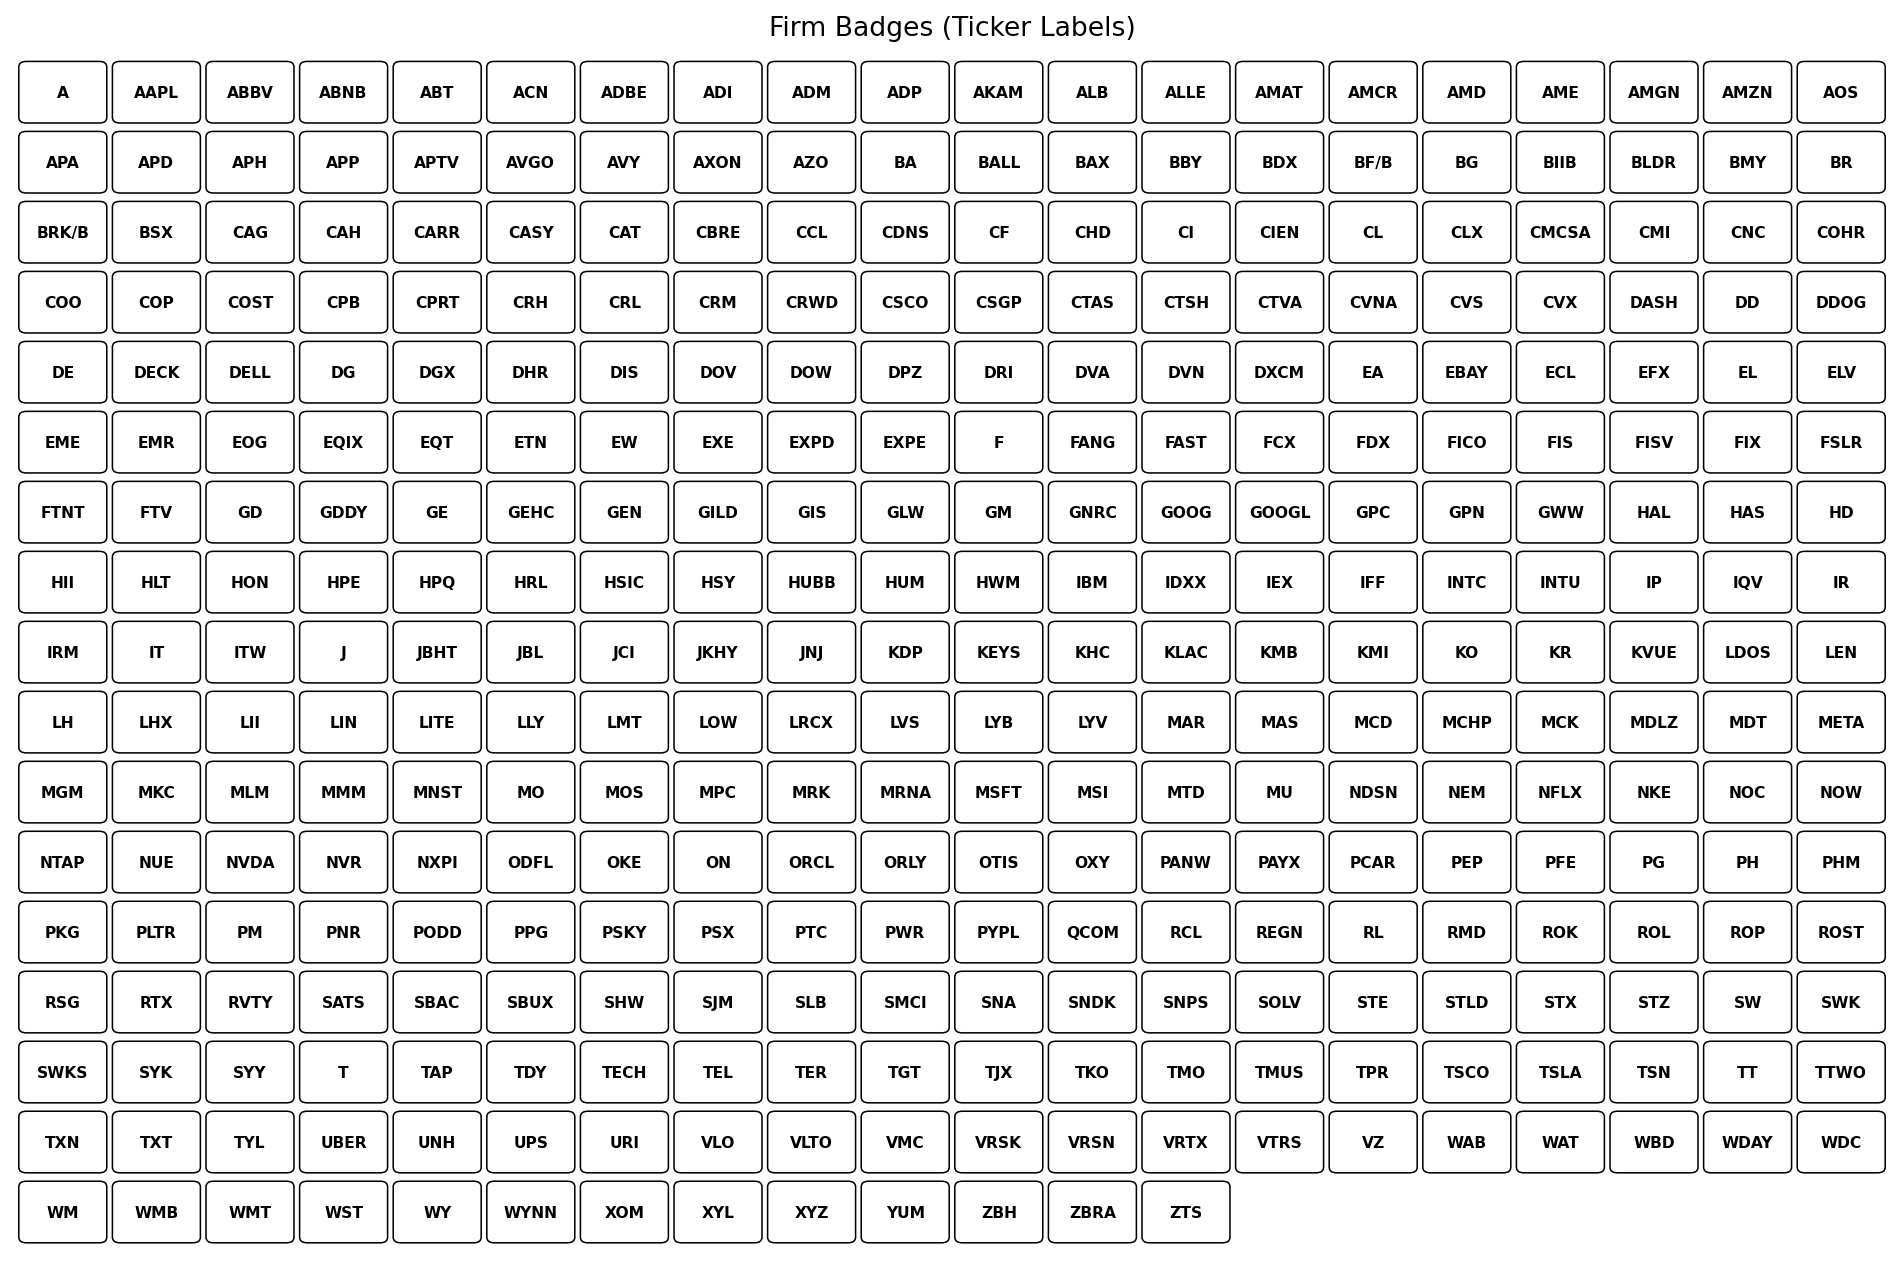
\includegraphics[width=0.92\textwidth]{../output/figures/firm_badges.png}
\caption{Badge Ticker Perusahaan Sampel}
\end{figure}

\begin{figure}[H]
\centering
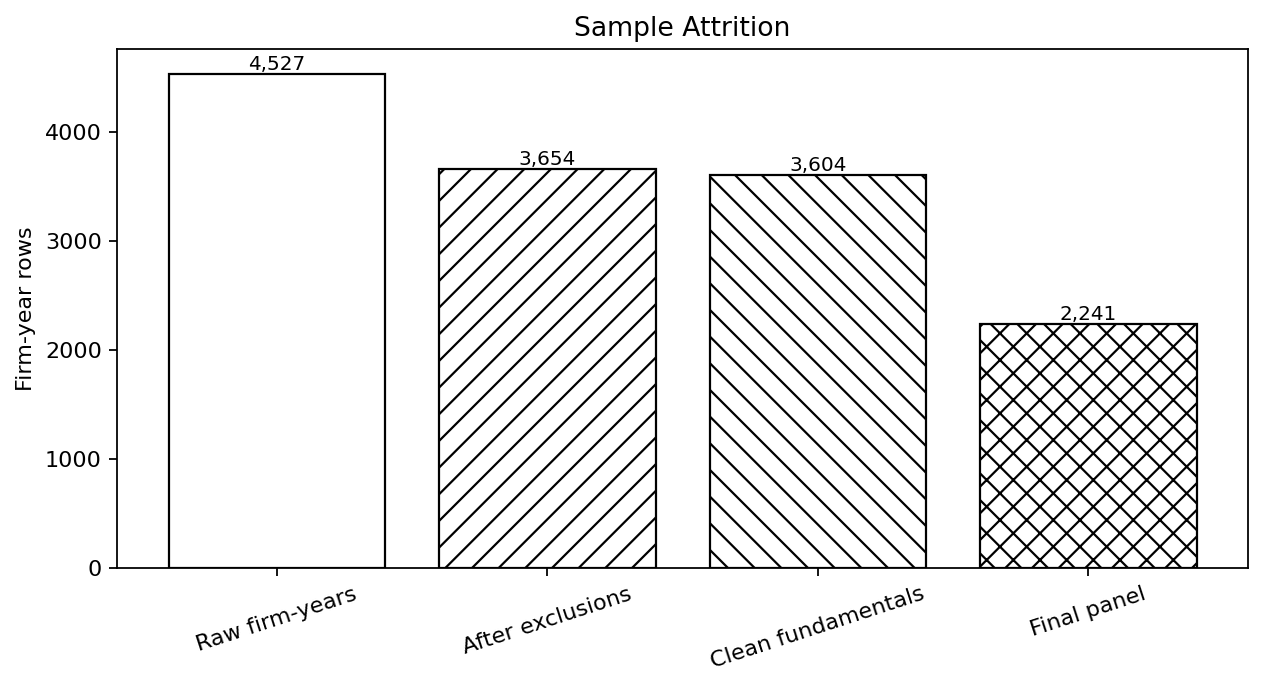
\includegraphics[width=0.92\textwidth]{../output/figures/sample_attrition.png}
\caption{Sample Attrition}
\end{figure}

\begin{figure}[H]
\centering
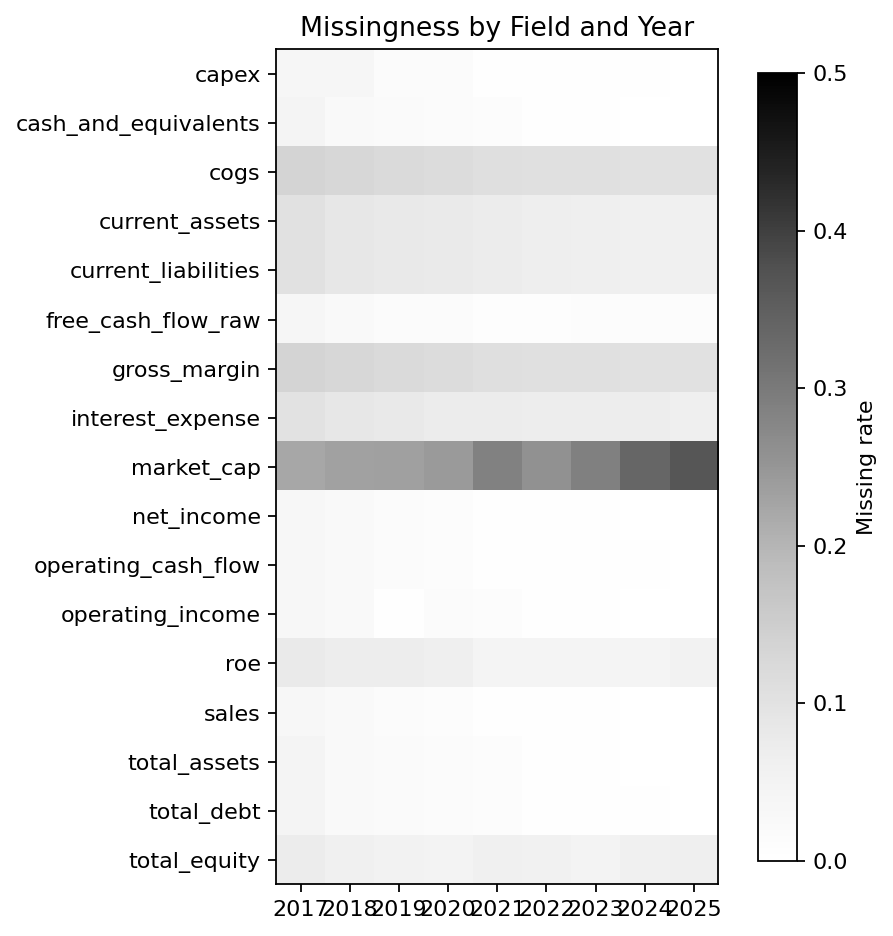
\includegraphics[width=0.92\textwidth]{../output/figures/missingness_heatmap.png}
\caption{Missingness Field Bloomberg}
\end{figure}

\begin{figure}[H]
\centering
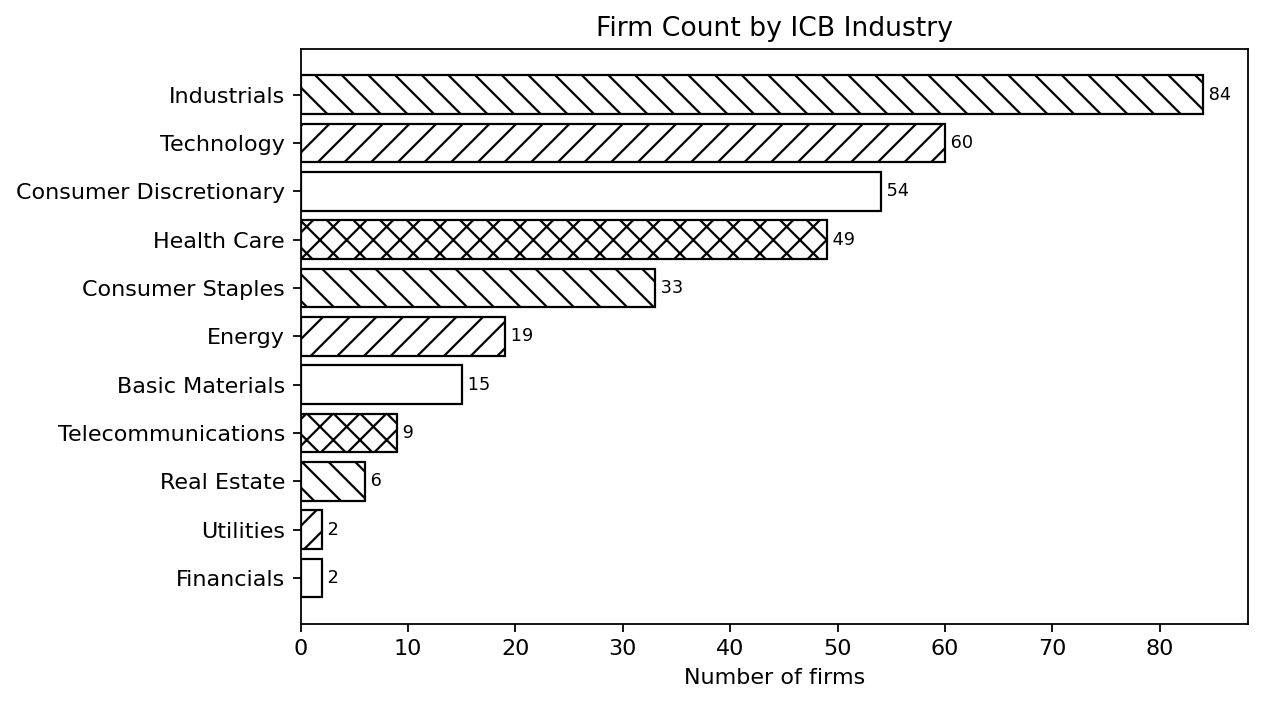
\includegraphics[width=0.92\textwidth]{../output/figures/industry_composition.png}
\caption{Komposisi Industri}
\end{figure}

\begin{figure}[H]
\centering
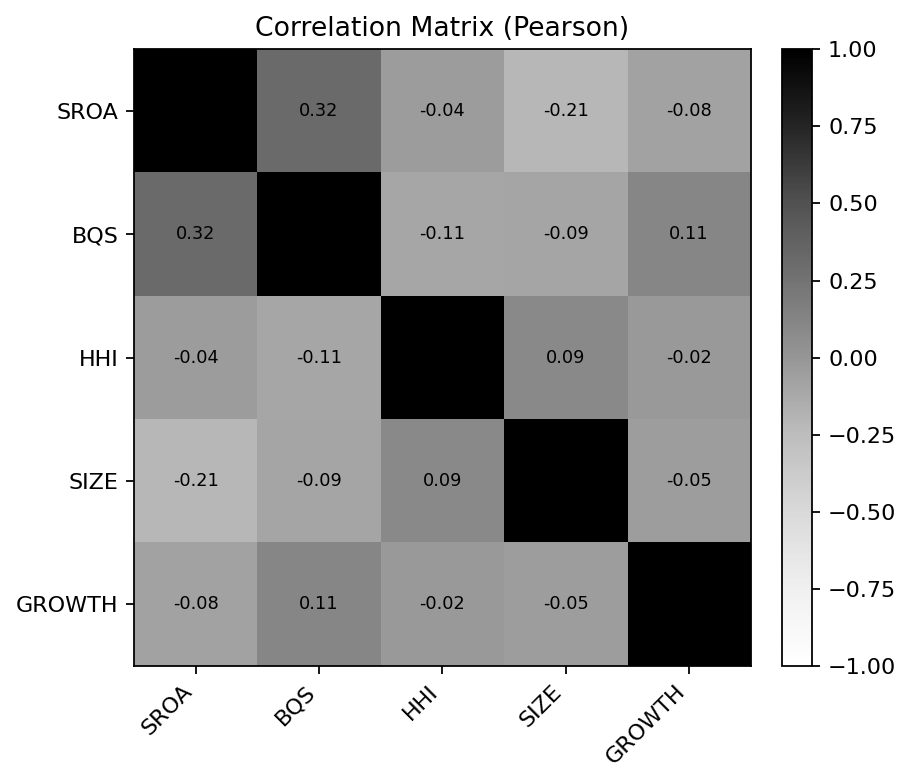
\includegraphics[width=0.92\textwidth]{../output/figures/correlation_heatmap.png}
\caption{Matriks Korelasi}
\end{figure}

\begin{figure}[H]
\centering
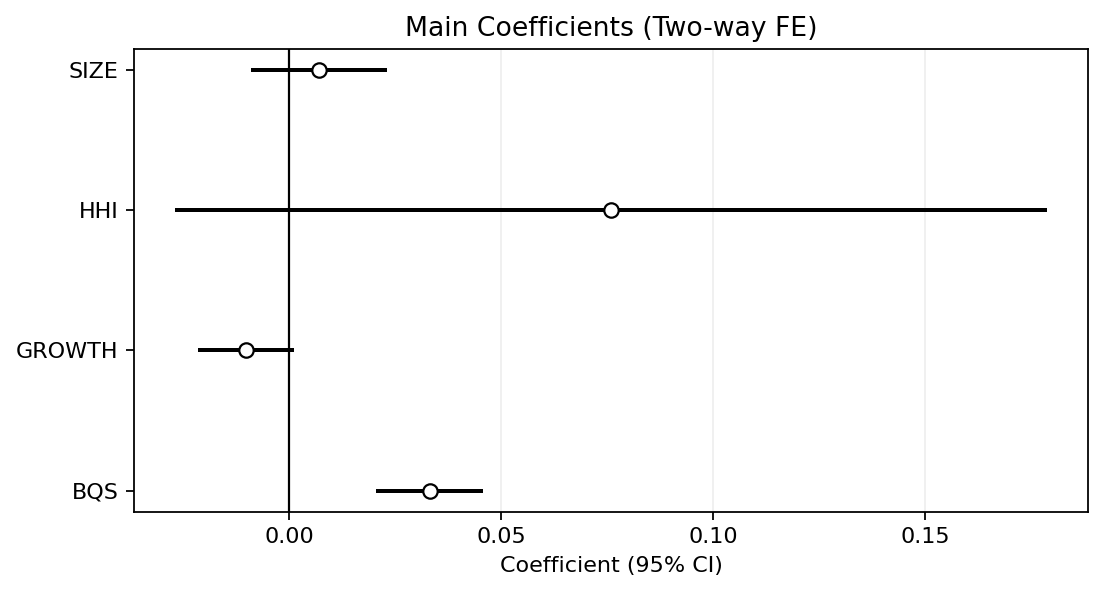
\includegraphics[width=0.92\textwidth]{../output/figures/coef_plot.png}
\caption{Plot Koefisien Model Utama}
\end{figure}

\begin{figure}[H]
\centering
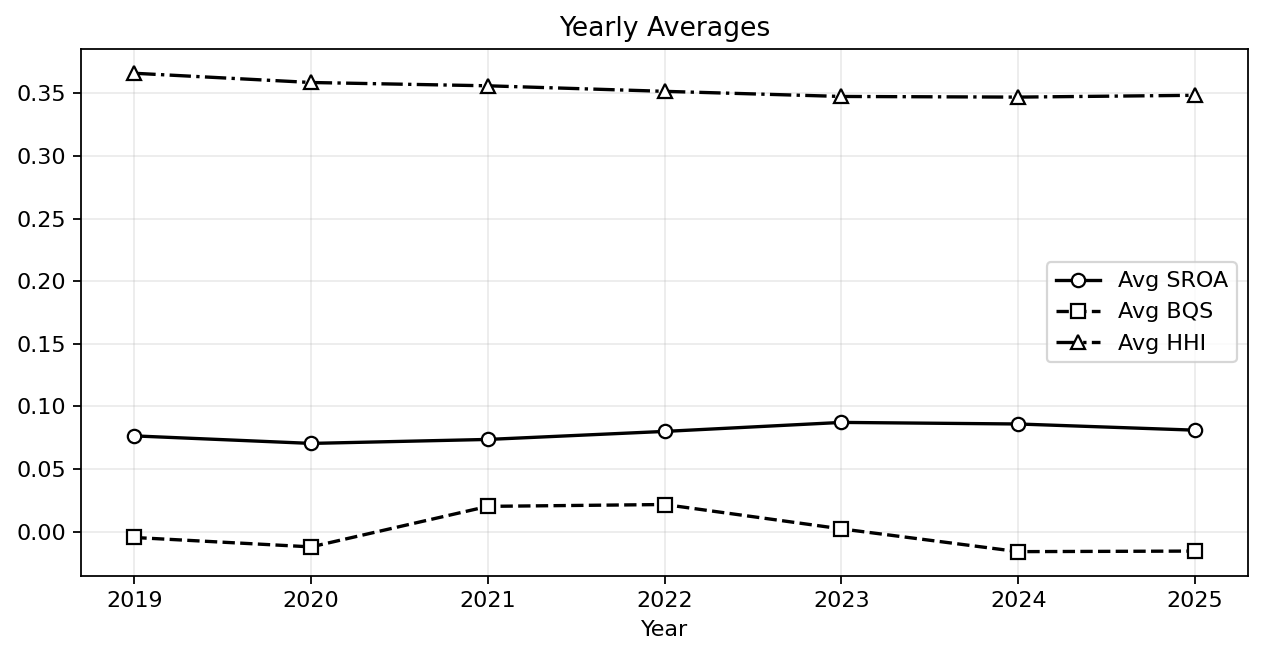
\includegraphics[width=0.92\textwidth]{../output/figures/trends.png}
\caption{Tren Rata-rata Tahunan}
\end{figure}

\begin{figure}[H]
\centering
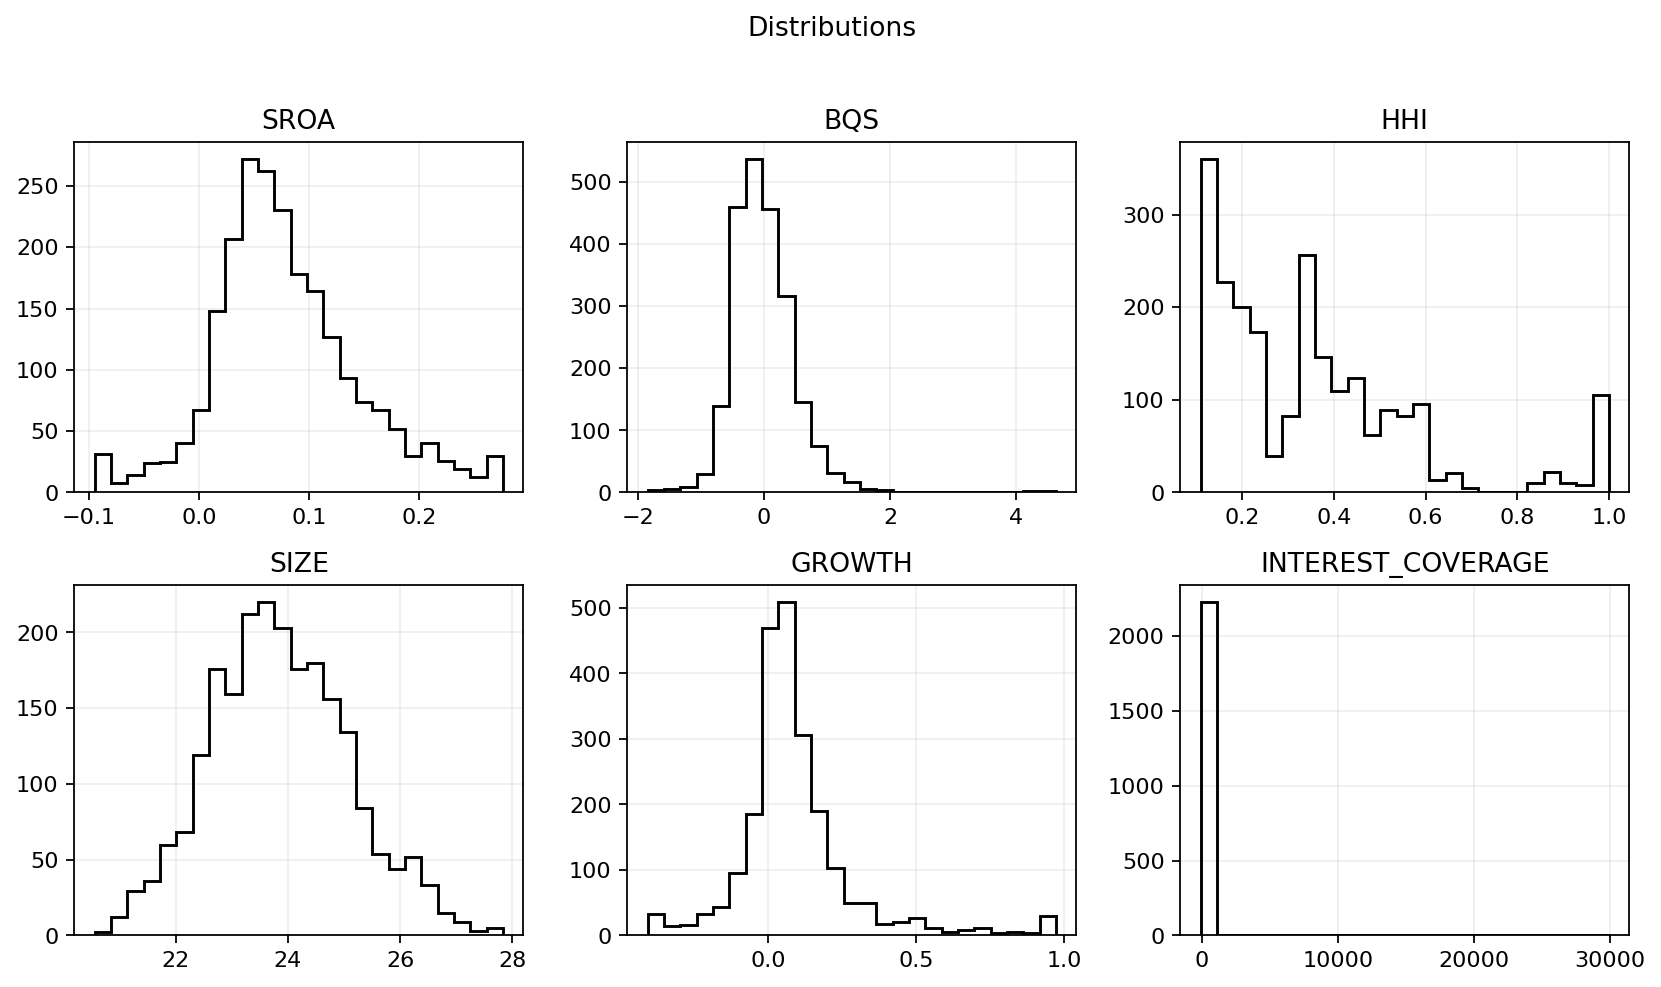
\includegraphics[width=0.92\textwidth]{../output/figures/distributions.png}
\caption{Distribusi Variabel Utama}
\end{figure}

\begin{figure}[H]
\centering
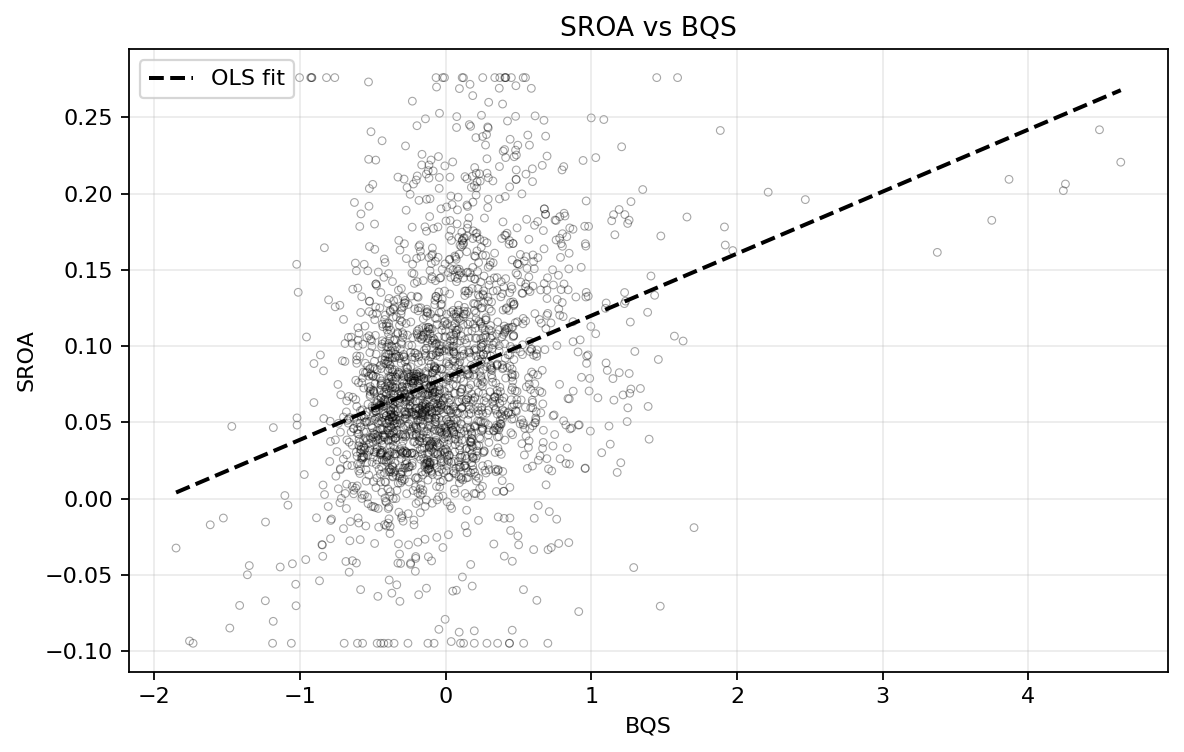
\includegraphics[width=0.92\textwidth]{../output/figures/scatter_sroa_bqs.png}
\caption{Scatter SROA dan BQS}
\end{figure}

\begin{figure}[H]
\centering
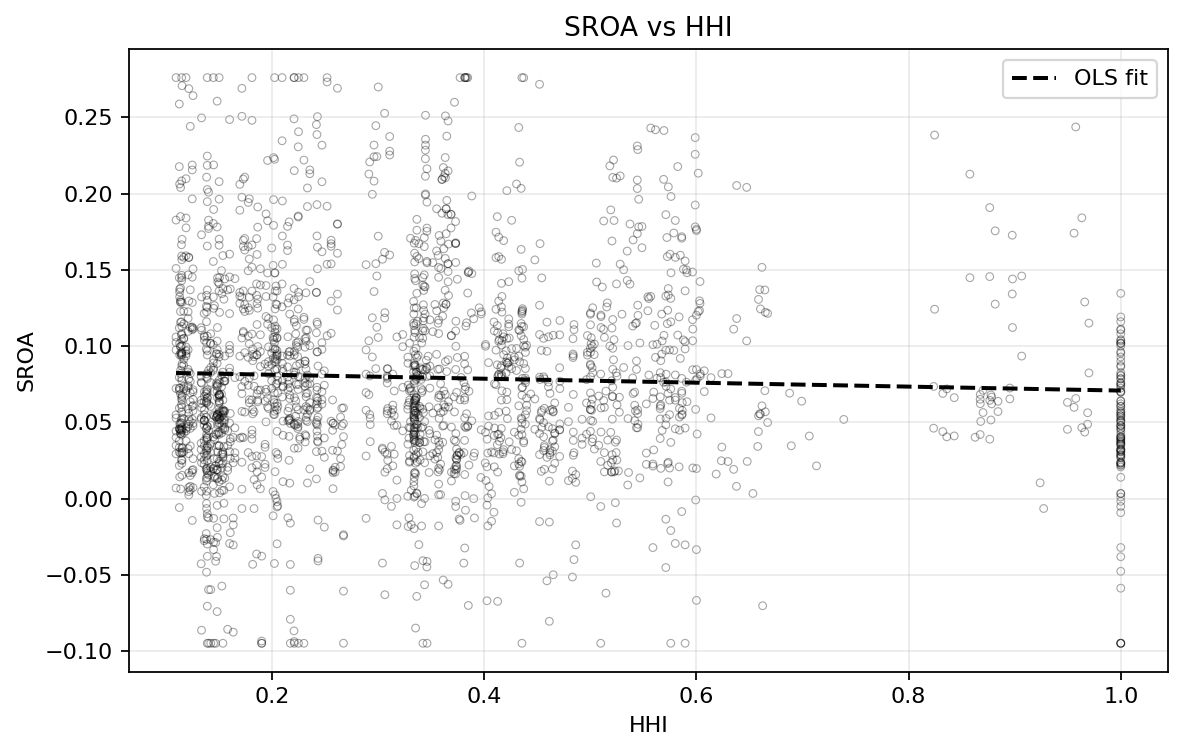
\includegraphics[width=0.92\textwidth]{../output/figures/scatter_sroa_hhi.png}
\caption{Scatter SROA dan HHI}
\end{figure}

\begin{figure}[H]
\centering
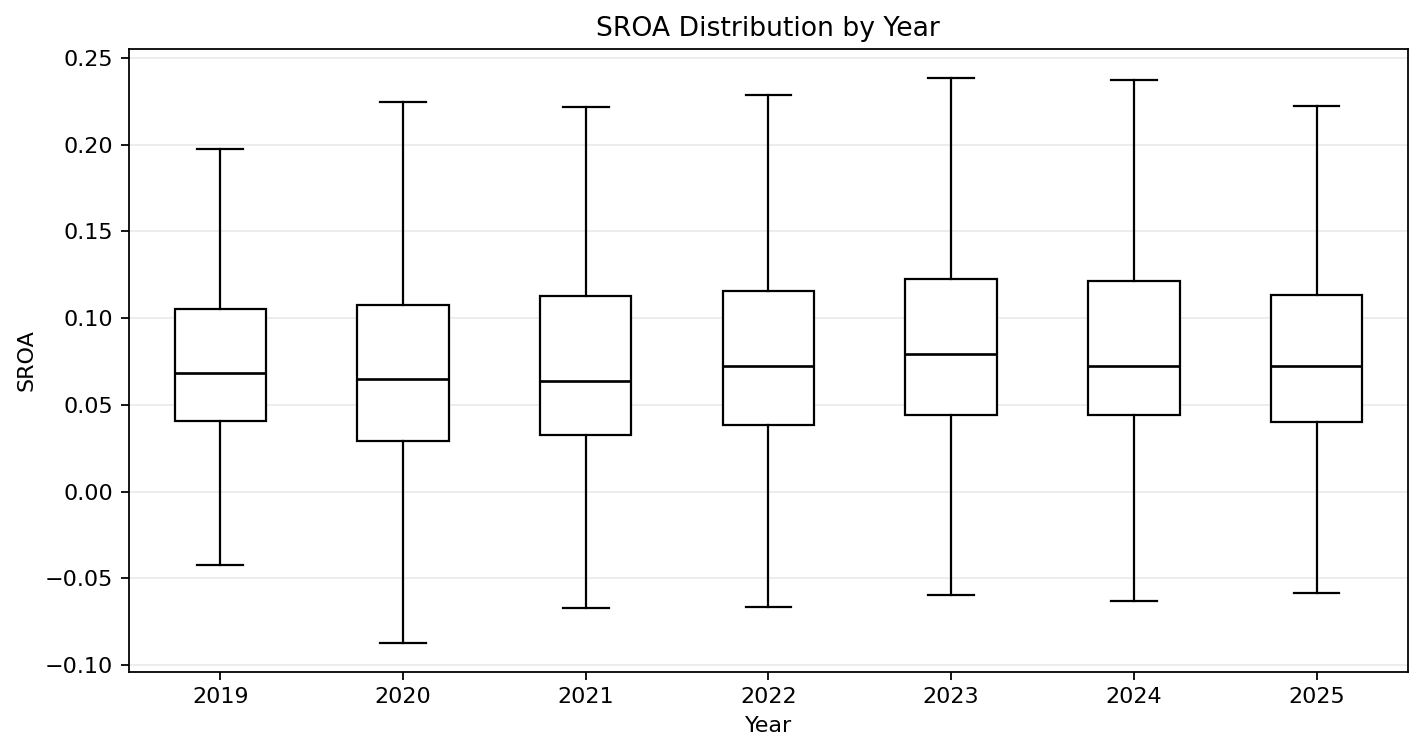
\includegraphics[width=0.92\textwidth]{../output/figures/box_sroa_by_year.png}
\caption{Boxplot SROA per Tahun}
\end{figure}

\begin{figure}[H]
\centering
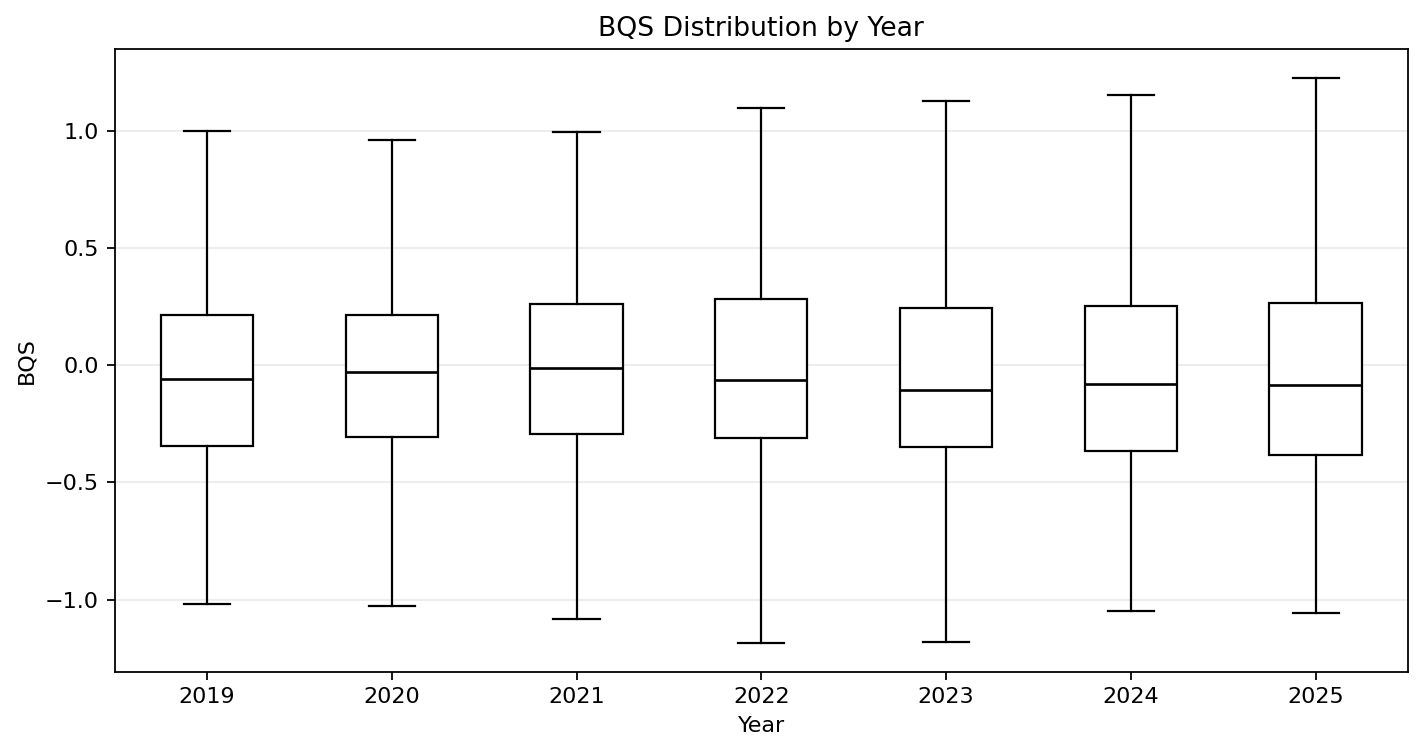
\includegraphics[width=0.92\textwidth]{../output/figures/box_bqs_by_year.png}
\caption{Boxplot BQS per Tahun}
\end{figure}

\begin{figure}[H]
\centering
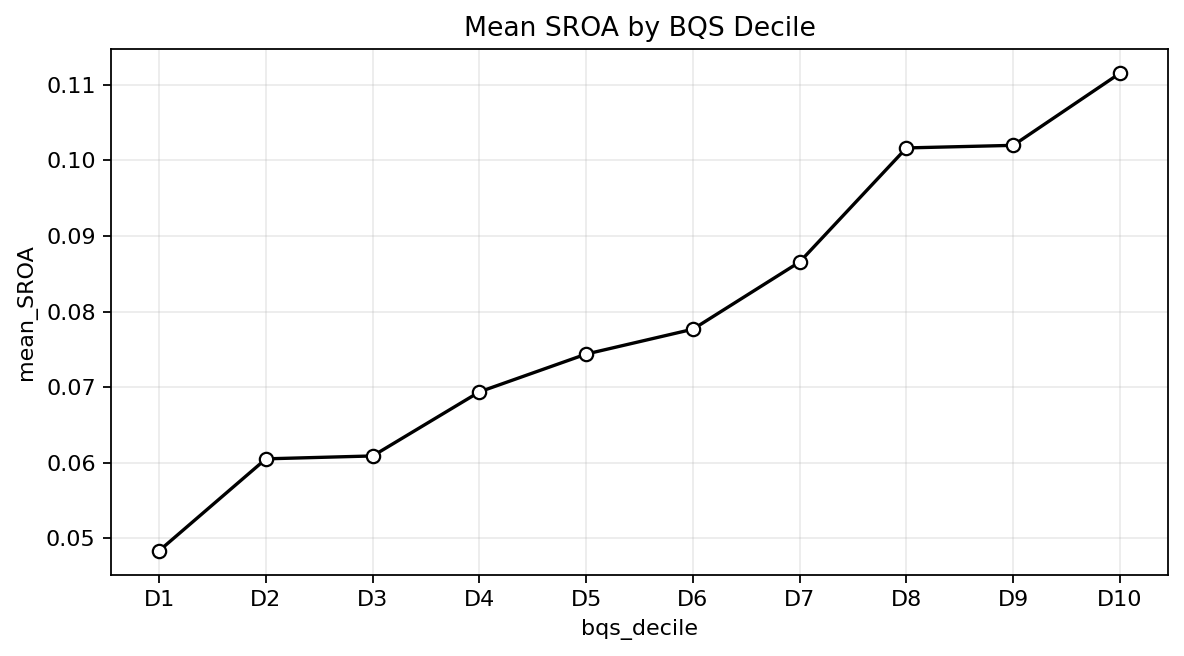
\includegraphics[width=0.92\textwidth]{../output/figures/sroa_by_bqs_decile.png}
\caption{Rata-rata SROA per Desil BQS}
\end{figure}

\begin{figure}[H]
\centering
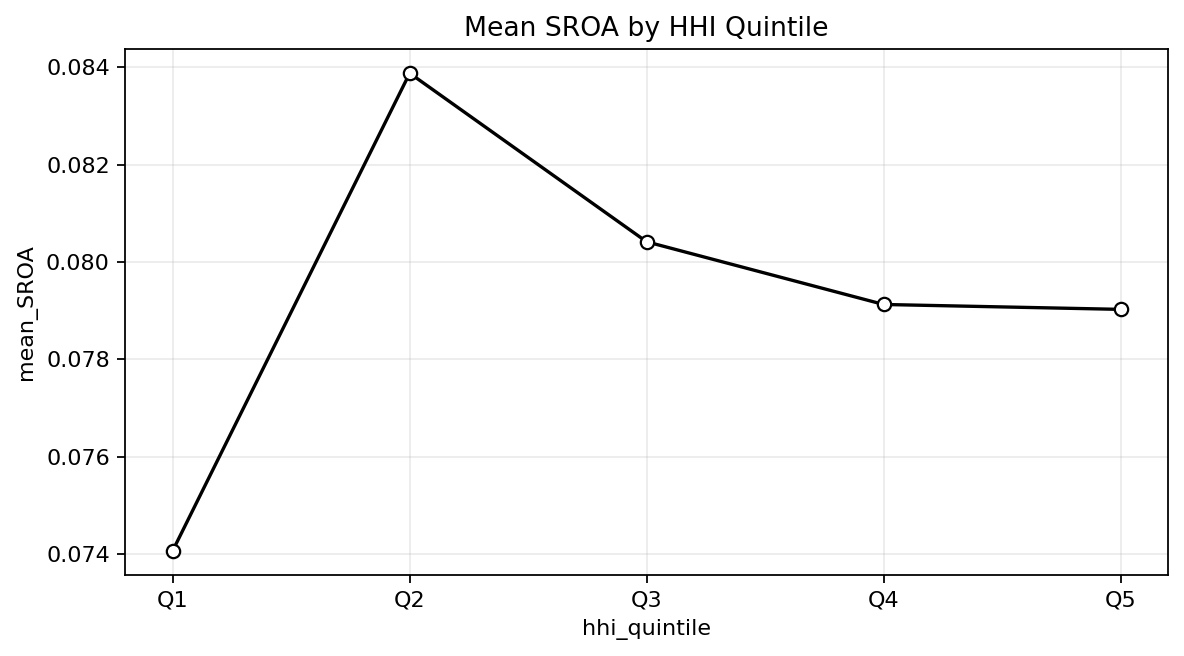
\includegraphics[width=0.92\textwidth]{../output/figures/sroa_by_hhi_quintile.png}
\caption{Rata-rata SROA per Kuintil HHI}
\end{figure}

\begin{figure}[H]
\centering
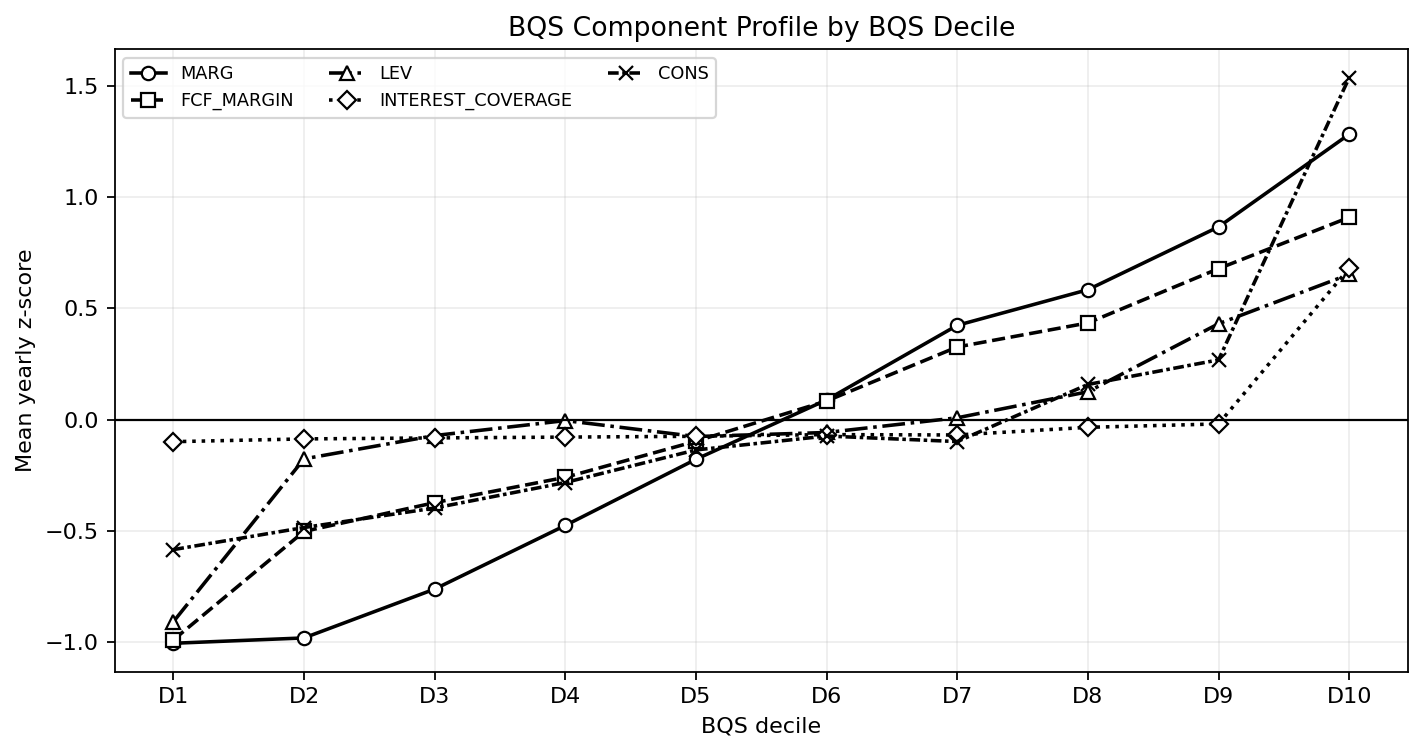
\includegraphics[width=0.92\textwidth]{../output/figures/bqs_component_profile.png}
\caption{Profil Komponen BQS}
\end{figure}

\begin{figure}[H]
\centering
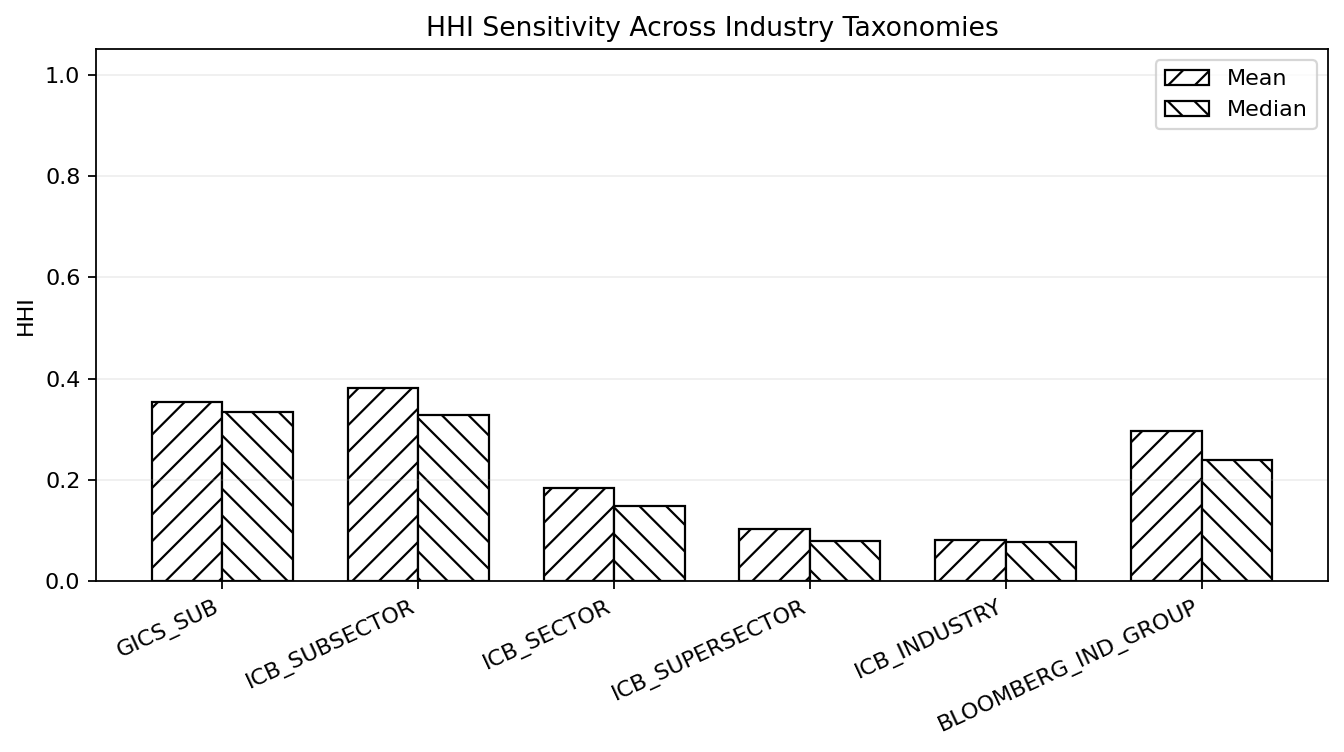
\includegraphics[width=0.92\textwidth]{../output/figures/hhi_taxonomy_comparison.png}
\caption{Perbandingan Taksonomi HHI}
\end{figure}

\begin{figure}[H]
\centering
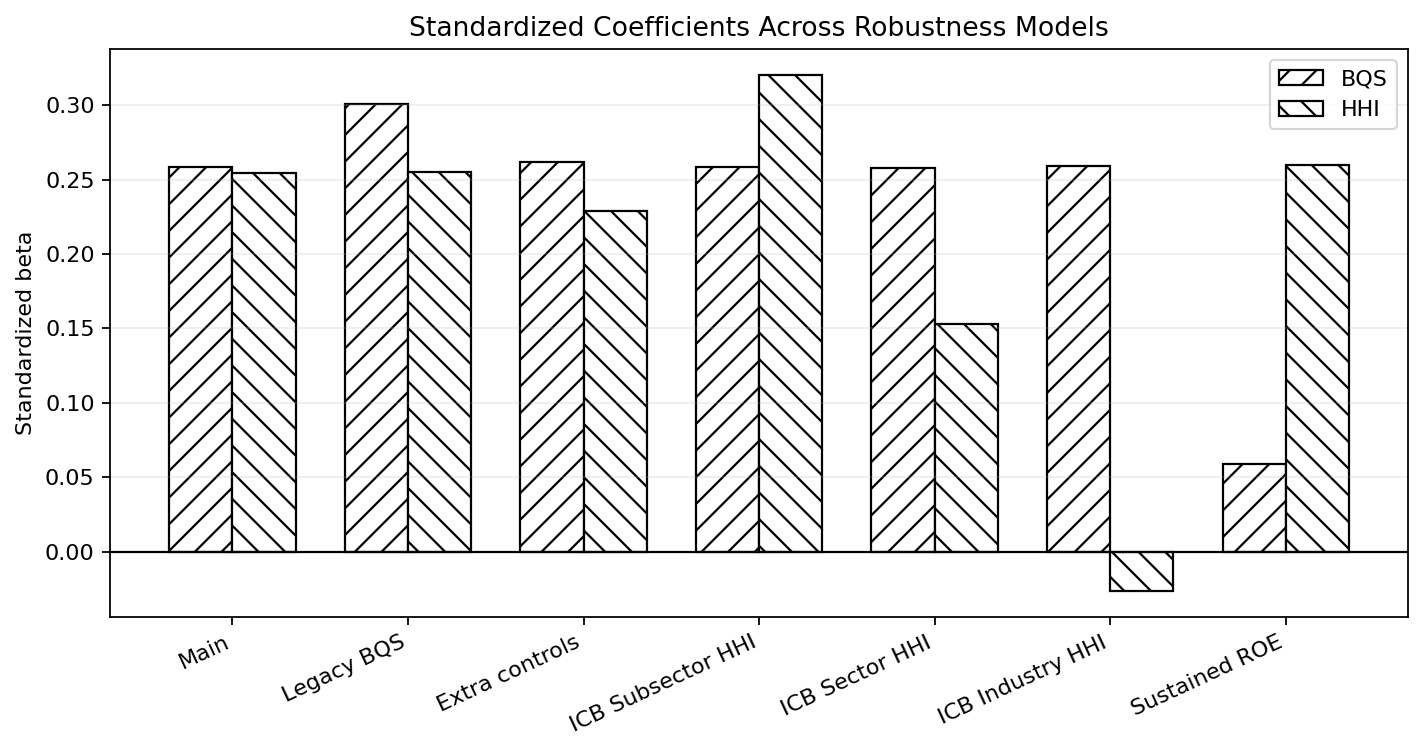
\includegraphics[width=0.92\textwidth]{../output/figures/coef_comparison.png}
\caption{Perbandingan Koefisien Robustness}
\end{figure}

\subsection*{\texorpdfstring{\textbf{Lampiran G Audit Data dan Pipeline
Pengolahan}}{Lampiran G Audit Data dan Pipeline Pengolahan}}\label{lampiran-g-audit-data-dan-pipeline-pengolahan}
\addcontentsline{toc}{subsection}{\textbf{Lampiran G Audit Data dan
Pipeline Pengolahan}}

Audit data final tersedia dalam berkas JSON pipeline pada folder data
dan output. Berkas audit tersebut mencatat jumlah perusahaan awal,
eksklusi Financials dan Utilities, missing values, kebijakan
complete-case BQS, serta rentang panel efektif yang digunakan dalam
regresi.

\end{document}
